%
\documentclass[letterpaper,11pt]{article}
%
% Place Encapsulated Postscript Illustrations
\usepackage{graphicx}
\usepackage{color}
%
% Place hyperlinks within the pdf file
\usepackage[colorlinks=true]{hyperref}
%
% Placing sub-figures within a figure float
\usepackage{subfigure}
%
% Rotate the figures so that they will fit on the page
\usepackage{rotating}
%
% Special labeling of enumerations
\usepackage{enumerate}
%
%Advanced mathematics formatting
\usepackage{amsmath}
%
\usepackage{etoolbox}
\makeatletter
\preto{\@verbatim}{\topsep=0pt \partopsep=0pt }
\makeatother
%
\newcommand{\Oval}{\textsc{Oval}}
\newcommand{\OvalPlot}{\textsc{OvalPlot}}
\newcommand{\Dempla}{\textsc{Dempla}}
\newcommand{\Ovalplot}{\OvalPlot}
\newcommand{\VersionA}{\Oval\texttt{-0.1.134}}
\newcommand{\VersionB}{\texttt{0.2.1}}
\newcommand{\Var}[2]{\texttt{#1}\ \  (\texttt{#2})}
\newcommand{\RunFile}{\textsf{RunFile}}
\newcommand{\StartFile}{\textsf{StartFile}}
\newcommand{\ConfigFile}{\textsf{ConfigFile}}
\newcommand{\BaseName}{\textsf{BaseName}}
\newcommand{\ColumnFile}{\textsf{ColumnFile}}
\newcommand{\LayerFile}{\textsf{LayerFile}}
\newcommand{\DFile}{\textsf{DFile}}
\newcommand{\GFile}{\textsf{GFile}}
\newcommand{\LFile}{\textsf{LFile}}
\newcommand{\MotionFile}{\textsf{MotionFile}}
%
\renewcommand\contentsname{\section{Contents}}
\renewcommand\refname{\section{References}}
%
\setlength{\textheight}{8.00in}
%
\newlength{\Labelwidth}
\setlength{\Labelwidth}{0.70in}
\newcommand{\Entrylabel}[1]{\makebox[\Labelwidth][r]{\texttt{#1}}}
%
\newenvironment{Options}
{\begin{list}{}{%
\renewcommand{\makelabel}{\Entrylabel}%
\setlength{\leftmargin} {0.90in}%
\setlength{\rightmargin}{0.00in}%
\setlength{\labelsep}   {0.10in}%
\setlength{\labelwidth} {\Labelwidth}%
}}
{\end{list}}
%
\newcommand{\Entrylabelnew}[1]{\makebox[\Labelwidth][l]{\texttt{#1}}}
\newenvironment{Options2}
{\begin{list}{}{%
\renewcommand{\makelabel}{\Entrylabelnew}%
\setlength{\leftmargin} {0.60in}%
\setlength{\rightmargin}{0.00in}%
\setlength{\labelsep}   {0.20in}%
\setlength{\itemindent} {1.50in}%
\setlength{\labelwidth} {1.50in}%
}}
{\end{list}}
%
% Chicago Manual of Style citation and bibliographic conventions.  I use this
% package because it closely mimics the Author-year citation style of
% "Mechanics of Materials".  It also allows context-sensitive modifications
% to the standard citation style.  In particular, I use \citeNP and \citeN
% in certain appropriate instances.  I occasionally use the \shortcite option
% to force use of "et al." in citations.  The month may sometimes
% appear along with the year in the bibliography (sorry!).
%
\usepackage{chicago}
% My package ASCE-like bibliographic entries
\bibliographystyle{ascelike}
%
%\markboth{\slshape\footnotesize\rightmark}{\thepage}
%\renewcommand{\sectionmark}[1]{\markright{\thesection\ #1}}
%
\begin{document}
%
% You will need to make the title all-caps
\title{\Dempla\ and \Oval:\\programs for analyzing
particle assemblies
and for simulating wave propagation and liquefaction
with the Discrete Element Method}
%
\author{
Matthew R. Kuhn%
\thanks{Dept. of Civil Engineering, Donald P. Shiley School of Engineering,
University of Portland,
5000 N. Willamette Blvd., Portland, OR 97203 USA,
\texttt{kuhn@up.edu}.}%
, \texttt{kuhn@up.edu}%
}
\date{\today\\ \Dempla\ version \VersionB}
%
\maketitle
%
\section{Introduction}
\Dempla\ means ``Discrete Element Method for Propagation
and Liquefaction Analysis.''
Two programs are included as two modes of the same \Dempla\ code.
The two modes incorporate the older code \Oval,
which serves as the underlying back-engine for
Discrete Element Method (DEM) simulations and
of individual particle assemblies and of the
multiple assemblies of a one-dimensional
soil column.
In the first mode,
the program \Oval\ 
(which is contained within the larger \Dempla\ code)
performs DEM analysis of a single particle assembly.
In the second mode,
\Dempla\ uses multiple DEM assemblies to analyze
one-dimensional wave propagation within a soil column.
The DEM is a method for
simulating the motions and interactions of the individual particles
in a granular material while the entire assembly is 
being deformed \cite{Cundall:1979a}.
Perhaps most important, the code allows extracting global averages
of such quantities as stress and fabric for the entire assembly
as well as the micro-level quantities, such as particle movements and contact
forces.
In the first mode,
the program is primarily intended for analyzing ``dense''
assemblies (as opposed to diffuse assemblies) 
that are roughly rectangular in shape, such as in so-call \emph{element tests}.
In the first mode, the code
can also be used to create assemblies by
compacting a diffuse assembly into a denser state.
The program's capabilities in this mode are summarized in
Section~\ref{}.
In the first mode, the code runs the DEM code with a single
computing thread.
\par
In the first mode,
the program handles both two-~and three-dimensional simulations
with particles that are either circles (2D), ellipses (2D), ovals (2D),
spheres (3D), 
``nobby'' clusters of circles (2D),
``bumpy'' clusters of spheres (3D),
a special non-spherical ``ovoid'' particle (3D).
%
\par
In the second mode,
the code uses 3D DEM assemblies as the representative
volume elements (RVEs) within a one-dimensional soil column
to analyze wave propagation
and liquefaction in the column.
In this mode, the code is
a multi-phase, multi-scale rational
method for modeling and predicting free-field wave propagation
and for modeling
the weakening and liquefaction of near-surface soils.
The one-dimensional time-domain
model of a soil column uses the discrete element method (DEM) to track
stress and strain within
a series of representative volume elements (RVEs),
driven by seismic rock displacements at
the column base.
The RVE interaction are accomplished with a
time-stepping finite-difference algorithm.
The method applies Darcy's principle to resolve the
momentum transfer between a soil's solid matrix and its
interstitial pore fluid.
Different algorithms are described for the dynamic period of seismic
shaking and for the post-shaking consolidation period.
%Although the paper is focus on the algorithm and its verification,
The method can analyze numerous conditions and phenomena,
including site-specific amplification,
down-slope movement of sloping ground,
dissolution or cavitation of air in the pore fluid,
and drainage that is concurrent with shaking.
Several refinements of the DEM are described for
realistically
simulating soil behavior and for solving a range
of propagation and liquefaction problems,
including the poromechanic stiffness of the pore fluid
and the pressure-dependent drained stiffness of the grain matrix.
The model is applied to the conditions of four sets of
well-documented centrifuge studies.
The verification results are favorable
and highlight the importance of the pore fluid conditions, such as
the amount of dissolved air within the pore water.
In the second mode, the several DEM algorithm can be
run with multiple computing threads to analyze the many
DEM assemblies (RVEs) in parallelized fashion.
%
\par
In the second mode,
other than being restricted to one dimension,
the method is quite general and allows one to model and understand
diverse conditions and phenomena:
(1)~three-dimensional motions of rock and soil,
propagating as both p-waves and s-waves;
%site-specific surface motions that differ from those of
%the underlying rock;
(2)~nearly arbitrary stress and strain paths during
ground shaking;
(3)~sloping ground surface with down-slope movement;
(4)~multiple stratigraphic soil layers;
(5)~sub-surface water table or complete submergence of the site;
(6)~sloping water table with down-dip seepage forces;
(7)~onset and depth of liquefaction;
(8)~saturated soil, dry soil, or quasi-saturated soil with entrained air
at a specified saturation;
(9)~dissolution or cavitation of entrained air;
(10)~effect of saturation on wave propagation and liquefaction;
(11)~effect of drainage that is concurrent with shaking;
(12)~pore fluid with a specified viscosity;
(13)~site-specific
amplification of surface accelerations relative
to those of the rock base;
(14)~pressure-dependence of wave speed
and the slowing of
waves as they approach the surface;
(15)~dilation and the coupling of s-waves and p-waves;
(16)~voids redistribution and
development of a water film beneath less permeable layers;
(17)~softening of soil during shaking,
with a slowing of wave speeds and shifting of frequency content due
to build-up of pore fluid pressures;
(18)~post-shaking consolidation and settlement;
(19)~post-consolidation reshaking and post-triggering behavior; and
(20)~relative rise of the water table during and after shaking.
The authors has not fully investigated most of the possibilities.
%
\par
The code is freely available on GitHub.
If you find opportunities to improve the code or if you find errors,
please let me know or fork the code and
augment or correct the code yourself.
The author
compiles the Fortran code on BSD Unix and Gnu Linux systems,
although the code can likely be compiled on windows systems, too.
%
\par
Besides the code, the GitHub repository also
contains sample assemblies, example problems, and
Octave code for analyzing results.
%
\par
The code is free software; 
you can redistribute it and/or
modify it under the terms of the GNU General Public License
as published by the Free Software Foundation; either version~2
of the License, or (at your option) any later version.
These programs are distributed in the hope that it will be useful,
but without any warranty; without even the implied warranty of
merchantability or fitness for a particular purpose.
See the GNU General Public License for more details.
You should have received a copy of the GNU General Public License
along with this program; if not, write to the Free Software
Foundation, Inc., 59 Temple Place---Suite 330,
Boston, MA  02111-1307, USA.
%
\pagebreak
\tableofcontents
%
\pagebreak
%\pagestyle{myheadings}
\section{Capabilities and limitations}\label{sec:Capabilities}
\subsection{Capabilities and limitations of the code}\label{sec:CapabilitiesOval}
The its current version the code has the following capabilities and
limitations:
\begin{enumerate}
\item
In the first mode
it can perform discrete element 
analysis on assemblies containing any one of the following particle
types:  circles (2D), ellipses (2D), ovals (2D), spheres (3D),
``nobby'' clusters of circles (2D),
``bumpy'' clusters of spheres (3D),
and non-spherical ``ovoids'' (3D).
In the second mode, only the 3D shapes can be used.
\item
At present, it works best with flat periodic boundaries 
on all sides of a two- or three-dimensional assembly.
For two-dimensional assemblies (in the first mode),
it can also use flexible boundaries;
with both two- or three-dimensional assemblies,
it can use rigid boundaries.
It can only analyze assemblies with parallel boundaries
(i.e. assemblies of 2D parallelogram and 3D parallelepiped shapes).
\item
The code is not intended for boundaries of arbitrary shape
or for arbitrary boundary conditions.
\item
The code is intended for dense (jammed) particle assemblies
that are slowly deformed at quasi-static rates.
Although the code can also model rapid flows and diffuse
assemblies, this purpose was not a primary concern in
the code's design.
\item
It can create output files of both macro-results and micro-results
for the DEM assemblies.
The macro-result files include information on stress and deformations.
The micro-result files give information on particle positions, particle 
orientations, contact forces, and system topology.
\item
In the second mode,
the program can create the same output files for each of the
DEM assemblies in the soil column, as well as average assembly
values of both the grain matrix and pore fluid for all
DEM assemblies along the height of the soil column.
\item
It includes a simple contact force mechanism consisting of linear springs 
(both normal and tangential) and
a frictional slider.  
The normal and tangential spring constants can
be specified independently (Sections~\ref{sec:kn} and~\ref{sec:kratio}).  
The frictional slider can be ``turned off''
(Sections~\ref{sec:frict} and~\ref{sec:frictw}).
\item
It also includes more advanced contact models:
Hertz-Mindlin models of sphere-sphere contacts, cone-cone contacts,
and contacts of intermediate shape (surfaces of revolution
of power-form contours).
With these models, the grains' shear modulus,
Poisson ratio, and friction coefficient must be specified.
\item
The code can analyze assemblies with a poromechanic description
of the pore fluid.
As such, the code directly computes the pore fluid pressure
as well as the inter-granular (effective) stress,
and it can adjust the inflow of pore fluid as well as the
deformation of the grain matrix.
\item
Available poromechanic models include dry assemblies,
saturated assemblies, and quasi-saturated assemblies in which
gas is presents as entrained bubble that do not form
a continuous network within the pore space separate from
the pore liquid.
\item
The following pore fluid characteristics can be specified:
saturation, bubble size or number density, gas solubility,
surface tension, liquid bulk modulus, etc.
\item
It includes the option of a modified DEM algorithm for self-regulating 
and maintaining
the quasi-static nature of a simulation (Sections~\ref{sec:algori},
\ref{sec:chi1}, \ref{sec:xloops}, and~\ref{sec:advice}).
\item
It includes the following types of damping:  
translational mass (global) damping,
rotational mass (global) damping, contact damping
(refer to \citeNP{Cundall:1979a}),
and the damping method of Potyondy and Cundall.  
Each may be
independently specified or ``turned off''
(Sections~\ref{sec:pcrit1}--\ref{sec:pcrit3}).
\item
It includes a robust servo-control 
algorithm for controlling the boundary stresses.
The deformation (or stress) path is supplied by the
user in a series of steps, which
specify in a component-by-component manner either the deformation rate 
tensor or stress rate tensor.  The specified stress or deformation rate 
components may be mixed.  See Section~\ref{sec:runfile2}.
\item
With stress-control, either the effective stresses or total stresses
can be controlled in arbitrary combinations.
\item
When a pore fluid is modeled, either the fluid pressure or
the fluid inflow can be controlled.
This capability is necessary for analysis wave propagation
and liquefaction in the second mode.
\item
It can create binary ``restart'' files that allow a new
simulation to begin at the exact ending condition
of a previous simulation.  These restart files include all of the position, 
velocity, and contact information that allow the new run to begin
where the previous run had stopped.
See Sections~\ref{sec:istart}, \ref{sec:iend}, and~\ref{sec:idump}.
\item
It can assign initial random velocities to the particles in
the assembly (Sections~\ref{sec:xseed} and~\ref{sec:rmsvel}).
\item
As an option, it can prevent particle rotations, particle motions, or both.
%\item
%It does not yet include gravity effects.
%\item
%The code is not yet parallelized.
\end{enumerate}
%
%
\subsection{Things to do}
Please help write this section.
%
%
%
\section{Availability and installation}\label{sec:installation}
The code is written in a rather inelegant dialect of Fortran 77.
The entire program and other files can be downloaded from the
GitHub repository,
including the source code, this documentation,
sample assemblies, and example problems.
Source code is freely available under terms of the open source GNU General
Public License (GPL), version~2.
\par
The program can be run in two modes.
Running \Dempla\ requires several input components:
\begin{enumerate}
	\item
	  In the first mode
	  (stand-along simulation of a single particle assembly),
	  the following input files are required:
	  \begin{itemize}
	     \item
	       The compiled executable file of \Dempla,
	       as described below.
	     \item
	       A \RunFile\ that specifies the contact model,
	       the poromechanic model (if any),
	       the general conditions of the simulation,
	       and the sequence of stress-strain control steps
	       to be performed by the simulation.
	     \item
	       A \StartFile\ that gives the size of the assembly,
	       the numbers of particles in the assembly,
	       and the locations, sizes and orientations of
	       all particles in the assembly.
	  \end{itemize}
    \item
      In the second mode (wave propagation and liquefaction
      analysis of a one-dimensional soil column),
      several input files are required.
      Many of these files must be arranged within a particular
      directory (folder) structures, described later.
      \begin{itemize}
      	\item
          The compiled executable file of \Dempla, as described below.
          The source code should be compile with the OpenMP parallelization
          library, as described below.
          Shell variables should also be set to permit multi-thread
          running of \Dempla, as described below.
        \item
          A \GFile\ that specifies the number of DEM assemblies
          in the soil column, the height of the column,
          the number of stratigraphic soil layers,
          water depth, and
          other general characteristics of the simulation.
        \item
          One \LFile\ for each of the stratigraphic soil layers,
          giving the \RunFile\ and \StartFile\ for setting up and running
          the DEM algorithm for the stratigraphic layer.
        \item
          A \RunFile\ for each stratigraphic layer
          that specifies the contact model,
          the poromechanic model (if any),
          the general conditions of the simulation,
          and the sequence of stress-strain control steps
         to be performed by the simulation.
        \item
          A \StartFile\ for each stratigraphic layer
          that gives the size of the assembly,
          the number of particles in the assembly,
          and the locations, sizes and orientations of
          all particles in the assembly.
        \item
          A \MotionFile\ that gives the displacement sequence
          at the base of the soil column.
      \end{itemize}
\end{enumerate}
%
%
\subsection{Compiling \Dempla\ on Linux systems}\label{sec:UnixSystems}
%
The following steps are required
to create a compiled executable \Dempla\ file and to set up
multi-thread running of the code (second mode, only).
If you are only running the program in first mode
(for a single assembly), only steps~1 and~2 are required,
and steps~3 through~6 can be ignored.
The author has compiled the code with both the \texttt{gfortran}
and \texttt{ifort} compilers.
If you compile with other compilers, please augment the descriptions
below with your own experience.
%
\begin{enumerate}
\item
Download or pull the following three files from the GitHub
repository:
  \begin{itemize}
  	\item
  	  \texttt{dempla-X.X.XX.f}, the latest version of the 
  	  main \Dempla\ source code.
  	\item
  	  \texttt{common-dempla-X.X.XX.f}, the corresponding file of
  	  the common blocks used throughout the \Dempla\ code.
  	\item
  	  \texttt{param-dempla-X.X.XX.f}, the corresponding file of
  	  parameters that sets the sizes of arrays in the \Dempla\ code.
  \end{itemize}
These three files should be placed in the same build folder.
%
\item
\Dempla\ can be parallelized by compiling with the proper OpenMP flag,
which for the gcc \texttt{gfortran} and Intel \texttt{ifort} compilers
are as follows:\\
\rule{3ex}{0ex} \texttt{gfortran}: \texttt{-fopenmp}\\
\rule{3ex}{0ex} \texttt{ifort}:    \texttt{-qopenmp}\\
To compile with optimization in the Linux shell:
\begin{verbatim}
    gfortran -std=gnu -O3 -mtune=native \
                       -mcmodel=large \
                       -fopenmp \
                       -o dempla.exe
                       dempla-X.X.XX.f
\end{verbatim}
or
\begin{verbatim}
    ifort -ipo -O3 -no-prec-div -fp-model fast=2 -xHost
          -fpconstant \
          -mcmodel=large \
          -qopenmp -heap-arrays \
          -o dempla.exe
          dempla-X.X.XX.f
\end{verbatim}
The options \texttt{-std=gnu -O3 -mtune=native} and
\texttt{-ipo -O3 -no-prec-div -fp-model fast=2 -xHost} produce
optimized code.
The options \texttt{-fltconsistency -fpconstant}
improve floating point precision.
Option \texttt{-mcmodel=large} is necessary
for large compiled arrays (as might be needed
when there are millions of particles or when there are
thousands of particles but with
the contact history parameter \texttt{mlistJ}
being exceptionally large).
The options \texttt{-fopenmp} and \texttt{-qopenmp}
specifiy compiling with the OpenMP library.
Option \texttt{-heap-arrays}
places temporary arrays that are used within subroutiens
(i.e., arrays that are treated as private and take new
values with each threaded instance) onto the heap instead
of the stack.
Finally, option \texttt{-o dempla.exe} specifies the
name of the executable file.
\par
To preclude parallelization and always run the code
as a single thread
(for example, with the first mode), simply
recompile dempla without the \texttt{-fopenmp}
or \texttt{-qopenmp} flags.
\par
Before compiling \Dempla,
you will need to consider the values of various
parameters that specify the sizes of arrays.
These parameters are described and given in the
file \texttt{param-dempla-X.X.XX.f}.
The most important parameters are \texttt{mp}
(the maximum number of particles in the DEM assemblies)
and \texttt{mrve} (the maximum number of DEM assemblies
(RVEs) in the soil column, when running the second mode).
For example,
if you are analyzing a soil column and wish to have
30 DEM assemblies in the column, you will need to
set \texttt{mrve=30} in the file \texttt{param-dempla-X.X.XX.f}
before compiling.
\par
Because the compile commands are cumbersome,
you might consider creating an \texttt{alias} within
the \texttt{.bashrc} configuration file.
%
\item
In order for parallelization to work within a Linux
shell (i.e., a terminal window),
you should specify number
of threads to be used during runtime inside of the shell.
The number of threads is given by
the shell environment parameter \texttt{OMP\_NUM\_THREADS}.
Within a Linux
bash shell:\\
\rule{3ex}{0ex}\texttt{export OMP\_NUM\_THREADS=4}\\
which would enable parallelized runs with 4 threads.
The authors typically uses 10 threads on a 28-thread Xeon processor.
This step must be done within \emph{every} shell (terminal)
within which the program is run,
or it can be included in the \texttt{.bashrc} file or in
another shell initialization script that can be sourced when needed.
Note that if no value of \texttt{OMP\_NUM\_THREADS} is set, then the
code will possibly run with all possible threads on the CPU,
which is usually not desirable.
\par
You can query the current value
of the environment parameter with this command:\\
    \rule{3ex}{0ex}\texttt{echo \$OMP\_NUM\_THREADS}
\par
To reset the \texttt{OMP\_NUM\_THREADS} parameter,
within a Linux bash shell:\\
\rule{3ex}{0ex}\texttt{unset OMP\_NUM\_THREADS}
\par
To query the number of threads available on the computer's hardware:\\
 \rule{3ex}{0ex}\texttt{lscpu | grep -E '\textasciicircum Thread|\textasciicircum
 Core|\textasciicircum
 Socket|\textasciicircum
 CPU\textbackslash('}
\par
See this guide for servers with multiple sockets, as with
Xeon and EPYC processors:\\
 https://software.intel.com/en-us/forums/intel-moderncode-for-parallel-architectures/topic/739878.
\par
Instead of setting the parameter
\texttt{OMP\_NUM\_THREADS}
in the shell, the
parameter can also be assigned at runtime.  For example,
if the executable code is 
\texttt{dempla.exe}, the following can
be run in the bash shell:\\
\rule{3ex}{0ex}\texttt{OMP\_NUM\_THREADS=4 ./dempla.exe}\\
when 4 threads are desired.
\item
For parallelized code, you might need to increase the stack
size to accommodate the multiple threads.  For example,\\
\rule{3ex}{0ex}\texttt{export OMP\_STACKSIZE=80m}\\
The default size of \texttt{OMP\_STACKSIZE=80m}
is usually small, 1m or 2m, and can lead
to segmentation fault errors during runtime.
You might need
to try different sizes, until an adequate stack size is found,
but without exhausting the machine memory.
See this explanation:\\
https://stackoverflow.com/
questions/13264274/
why-segmentation-fault-is-happening-in-this-openmp-code
\par
The parameter can also be assigned at runtime.
In the bash shell:\\
\rule{3ex}{0ex}\texttt{OMP\_NUM\_THREADS=4 OMP\_STACKSIZE=80m ./dempla.exe}
%
\item
One must provide sufficient memory for parallel execution.
The \texttt{gfortran} and \texttt{ifort}
compilers create executable programs
that use stack memory instead of static memory.
The limit on stack memory size will need to be increased.
With Linux,
use the following shell command:\\
\rule{3ex}{0ex}\texttt{ulimit -s unlimited}
\par
This command must be entered in any shell that will run the
executable program, or it can be included in the .bashrc or other
shell initialization script.  Without this command, you will
likely receive a segmentation fault error.
%
\item
Finally, because of the many niggling steps that
are required to prepare a Linux shell to run parallelized
\Dempla, you might consider placing all of these
commands in a single Linux bash script file that can
be sourced within a terminal.
I use the following file \texttt{dempla.bsh} for setting up
the use of \Dempla\ in a bash shell:
\begin{verbatim}
   #!/bin/bash
   #
   ulimit -s unlimited
   export OMP_STACKSIZE=80m
   export OMP_NUM_THREADS=10
\end{verbatim}
but you will want to customize your own script and place it
somewhere within your shell's \texttt{\$PATH}.
\par
To run the script in shell, it must be sourced within the shell:\\
\rule{3ex}{0ex}\texttt{source dempla.bsh}
%
\end{enumerate}
%
\subsection{macOS systems}
Please help to write this section.
%
\subsection{Windows systems}
Please help to write this section.
%
%
\section{Helpful/essential utilities}\label{sec:Utilities}
Please help to write this section.
%
%
\section{Running \Dempla\ and \Oval} \label{sec:RunOval}
\Dempla\ is \emph{not} yet an interactive program with a graphical
user interface.
At present, it runs only in a batch mode.
%
\par
You would normally run \Dempla\ (in either of the two modes)
from within a terminal (e.g. an Linux xterm window, the
MacOS terminal utility,
or DOS console) with the following command at the system prompt:
\begin{verbatim}
    <path><dempla_executable_name>
\end{verbatim}
where \texttt{<path>} is the path to your executable
file with its \texttt{<dempla\_executable\_name>}
(e.g. \texttt{dempla.exe} or whatever
name or symbolic link is given to the file).
In the GitHub filesystem,
a Linux executable file '\texttt{dempla.exe}'
is located in the \texttt{bin/} directory.
Instead of explicitly providing the \texttt{<path>}, you may wish to
create a link (shortcut) to the \texttt{dempla} execturable file
(say, \texttt{dempla.exe}),
place the file it in a directory in your system's search \texttt{\$PATH}, 
or modify your system's search \texttt{\$PATH} to include
the directory that contains the \texttt{dempla} executable file.
\par
After starting the \texttt{dempa} command, you
will be queried for the run mode:
%
\begin{verbatim}
    Mode: single-assembly (1) or wave propagation (2):
\end{verbatim}
%
After entering the mode, you will be queried for various names
and information, which will
depend on the mode:
%
\begin{itemize}
  \item
	In the first mode (\texttt{imode=1}, single-assembly mode),
    you will be queried for the names of two
    files,
    \begin{verbatim}
      Name of the RunFile:
      
      Name of the StartFile:
    \end{verbatim}
    and the simulation will proceed to run.
    We will henceforth refer to these two files 
    with the generic names ``\textsf{RunFile}'' and
    ``\textsf{StartFile}'', which are described in
    Sections~\ref{sec:RunFile} and~\ref{sec:startfileD}.
    These two files must be created before running
    \Dempla.
    The file names of the \RunFile\ and \StartFile\ must
    conform to Unix conventions
    (no spaces, asterisks, question marks, etc.)
    The \RunFile\ must reside within the directory from
    which the \Dempla\ is run.
    The \StartFile\ can be located in another directory,
    in which case, you must enter the full path of the
    \StartFile.
    \par
    The output will normally be written to a set of files,
    whose names will
    contain the core \textsf{RunFile} name.
    The various output files are listed in
    Table~\ref{table:files} and 
    will be described later in the documentation.
    In the first mode, the output files are all placed within
    the directory in which \Dempla\ is run.
    \par
    As an example,
    the output file \mbox{\texttt{A<}\textsf{RunFile}\texttt{>.txt}}
    will be created, noting that
    the name of this output file contains
    the core \RunFile\ name.
    The file is created in the same director from which the
    \Dempla\ program is run.
    This ``\texttt{A}'' file
    is a text file that can be imported into a spreadsheet, such as
    Excel or Gnumeric to view the average stresses and deformations
    of the assembly (note, \emph{imported}, not opened).
    The file can also be read into Octave or Matlab with a utility function.
    \par
    Before describing the detailed contents of the \textsf{RunFile}
    and the \textsf{StartFile}, you should know
    that the \textsf{RunFile}
    is an ASCII (text) file that describes
    how the simulation is to be run:
    boundary deformation rates, boundary stress rates,
    friction coefficients, spring constants, etc.
    (see Section~\ref{sec:RunFile}).
    A \textsf{StartFile} gives the number of particles, particle type,
    and the initial particle arrangement (sizes, positions, etc.,
    see Section~\ref{sec:startfileD}).
    A \textsf{StartFile} may be of either ASCII or binary type
    (Table~\ref{table:files}).  
  \item
    Before you can run \Dempla\ in the second mode
    (i.e. to simulate wave propagation),
    you must create a special directory structure that will
    hold the input files and output files.
    This directory structure must be created inside of
    the directory in which \Dempla\ is being run.
    Three of these directories and their contents are
    as follows:
%
    \begin{itemize}
      \item
        A directory named \texttt{MotionInput}.
        This directory contain the input motion
        file, which describe the base (rock) motion
        for the simulation.
        A \MotionFile\ is a text file, having the
        format described in Section~\ref{}.
        The directory \texttt{MotionInput} can either
        be a directory with that name or a symbolic link
        (with the name \texttt{MotionInput}) targeting
        a directory that contains the \MotionFile.
      \item
        A directory named \texttt{RunFiles} that
        contains all of the \RunFile s that are used in
        the simulation.
        Each stratigraphic layer will have a \RunFile.
        Each \RunFile\ should reside inside the
        folder \texttt{RunFiles}.
        A \RunFile\ is a text file with
        contents and format described in Section~\ref{sec:RunFile}.
        The \RunFile\ describes
        the conditions under which the
        assemblies within the layer will be initialized
        and run:
        contact models,
        friction coefficients, spring constants,
        poromechanic fluid properties, etc.
        The names of \RunFile s must conform
        to Unix conventions.
        The directory \texttt{RunFiles} can either
        be a directory with that name or a symbolic link
        (with the name \texttt{RunFiles}) targeting
        a directory that contains the \RunFile s.
      \item
        A directory named \texttt{StartFiles} that
        contains all of the \StartFile s that are used
        in the simulation.
        A \StartFile\ is a text file with
        contents and format described in Section~\ref{}.
        Each \StartFile\ is a text file (a \DFile) that
        gives information about the particle assembly
        at the start of a simulation:
        assembly size, number of particles, and
        particle sizes, locations, and orientations.
        Each stratigraphic layer will have a \StartFile.
        Each \StartFile\ should reside inside the
        folder \texttt{StartFiles}.
        The names of \StartFile s must conform
        to Unix conventions.
        The directory \texttt{StartFiles} can either
        be a directory with that name or a symbolic link
        (with the name \texttt{StartFiles}) targeting
        a directory that contains the \StartFile s.
    \end{itemize}
%
    The above three directories have have general role,
    since many simulations can reference these directories
    and can be run inside of the directory that contains
    them (i.e., the directory in which \Dempla\ is being run).
    Besides the three directories, you must also create
    a directory that will contain input information and output
    for simulations on a particular soil column,
    noting that
    different input motions can be applied to the same
    soil column.
    A directory must be created with the \BaseName,
    which must conform with the Unix naming conventions.
    The \BaseName\ directory must also contain the following
    contents:
    \begin{itemize}
      \item
        The \BaseName\ directory must contain three sub-directories
        with the following names:
        \texttt{02\_LayerSetup}, \texttt{03\_RVESetup},
        and \texttt{04\_RunOutput}.
        These three sub-directories will be used to hold
        pre-processing files and the output files that are
        created by the simulations.
        Various output files will be placed inside the
        sub-directory \texttt{04\_RunOutput}, and these
        output files will be given names that contain
        the \BaseName\ and the name of the \MotionFile,
        so that the output sub-directory can contain
        output from multiple simulations, each with a different
        input motion.
        The various output files contain pore fluid pressures,
        soil displacements, effective stresses, etc.
        The range, format, and content of the various output files
        are described in Section~\ref{}.
      \item
        The \BaseName\ directory must contain a file that gives
        general information about the soil column:
        the number of DEM assemblies (RVEs) along the height,
        the number of stratigraphic layers, the column height,
        water depth, etc.
        This \ColumnFile\ must have the name
        \texttt{G}\BaseName\texttt{<suffix>}, noting the
        ``\texttt{G}'' prefix.
        As such, we refer to this file with the interchangeable
        references \ColumnFile\ and \GFile.
        The format and content of \GFile s are described
        in Section~\ref{}.
        The name of the \GFile\ can include an optional prefix
        (several simulations can be run with the same
        \BaseName\ and input motion, but can differ by the
        pore fluid saturation, and these variations can be
        distinguished with the suffix.  See Section~\ref{}).
      \item
        The \BaseName\ directory must also contain files that
        give information about all of the stratigraphic soil
        layers that are within the soil column.
        One \LayerFile\ must be created for each of the soil
        layers
        (note that the water table can be within the thickness
        of a soil layer, but only one \LayerFile\ is required
        for the layer).
        The \LayerFile\ must have the name
        \texttt{L<XXXX>\_}\BaseName.
        The name begins with letter ``\texttt{L}'',
        followed by a 4-digit number
        (beginning with \texttt{0001} for the top soil layer,
        and increasing with \texttt{0002}, \texttt{0003}, etc.
        to the bottom layer).
        The number is followed by an underscore ``\texttt{\_}''
        and the \BaseName.
        \par
        We will refer to this file with the interchangeable
        references \LayerFile\ and \LFile.
        The format and content of \LFile s are described
        in Section~\ref{}.
        The \LFile\ gives the thickness of the layer,
        void ratio, etc.
        Most important, the \LFile\ also gives the names of the
        \RunFile\ and \StartFile\ for the layer.
        \par
        The \RunFile\ for a layer
        provides general information about the
        DEM assembly that represents the particular stratigraphic
        layer.
        The \RunFile must be contained in the \texttt{RunFiles}
        directory (i.e., one of the three general sub-directories,
        described earlier).
        A \RunFile\ is a text file with
        contents and format described in Section~\ref{sec:RunFile}.
        The \RunFile\ describes
        the conditions under which the
        assemblies within the layer will be initialized
        and run:
        contact models,
        friction coefficients, spring constants,
        poromechanic fluid properties, etc.
        The names of \RunFile s must conform
        to Unix conventions.
        \par
        The \StartFile\ for a layer gives information
        about the size of the DEM assembly that represents
        the soil layer, along with the shapes, locations, sizes,
        and orientations of all of the particles in the assembly.
        A \StartFile\ is a text file with
        contents and format described in Section~\ref{}.
        Each stratigraphic layer will have a \StartFile.
        Each \StartFile\ should reside inside the
        folder \texttt{StartFiles}.
        The names of \StartFile s must conform
        to Unix conventions.
    \end{itemize}
%
    To run \Dempla\ in the second mode (multi-assembly wave
    propagation),
    start the program and enter 2 as the mode.
    You will be queried for the following three names,
    \begin{verbatim}
    	BaseName of the simulation (main folder name):
    	
    	Suffix of variation (if none, press return):
    	
    	MotionFile (name of rock motion file):
    \end{verbatim}
    and the simulation will proceed to run.
\end{itemize}
%
\begin{table}
\centering
\begin{tabular}{llll}
\hline
\hline
File name & Type & Function & Sections\\
\hline
\texttt{A<}\textsf{RunFile}\texttt{>.txt} & text   & 
macro-results for spreadsheets & \ref{sec:Afiles} \\
\texttt{B<}\textsf{RunFile}\texttt{>}     & text   & 
macro-results for text editors & \ref{sec:Bfiles} \\
\texttt{C<}\textsf{RunFile}\texttt{>}     & binary & 
 restart \textsf{StartFile}    & \ref{sec:istart} \\
\texttt{C?<}\textsf{RunFile}\texttt{>}     & binary & 
 restart \textsf{StartFile}    & \ref{sec:idump} \\
\texttt{D<}\textsf{RunFile}\texttt{>}     & text   & \textsf{StartFile} &
 \ref{sec:startfileD} \\
\texttt{F[1-4]?<}\textsf{RunFile}\texttt{>}& text   & micro-results 
for post-analyses & \ref{sec:ffiles} \\
\hline
\multicolumn{4}{p{4.50in}}
{?\ -- a letter that corresponds to the deformation-stress path in which
the file was created (Section~\ref{sec:idump} and
Section~\ref{sec:gfiles})}\\
\hline
\hline
\end{tabular}
\caption{\Oval\ output files}
\label{table:files}
\end{table}
%
\section{Boundary Types}\label{sec:Boundaries}
\Oval\ is primarily intended for element studies of using rectangular (2D) and
box (3D) assemblies of particles.
During a simulation, the boundaries (sides) are moved to produce
prescribed rates of strain or rates of stress, as described in 
Section~\ref{sec:runfile2}.
The boundaries themselves can be of several types.
%
\subsection{Periodic boundaries}\label{sec:Periodic}
The default boundaries are periodic.
These are the easiest boundaries to use, 
and they can be used with either dense or sparse assemblies.
Moreover, some of the other types of boundaries are created by starting
with an assembly having periodic boundaries and then replacing the
periodic boundaries with the another boundary type.
%
\subsection{Tight-fitting particle boundaries}\label{sec:TightFitting}
This type of boundary can only be created with 2D assemblies,
and it is created by beginning with a non-sparse (at least, moderately
dense) assembly having periodic boundaries.
The process of creating a tight-fitting particle boundary involves
finding the particle graph of the assembly (i.e., finding the
topological arrangement of the contacts) and then identifying the string
of contacting particles that surround the assembly.
These particles become the boundary particles, which will fit tightly
against (i.e., will be in contact with) the interior particles.
After the periodic boundaries are ``broken'' and replaced with
tight-fitting boundaries, the boundary particles will not likely be
in equilibrium, so a period of several hundred time steps should be
included to allow the assembly to equilibrate with its new boundaries.
Once periodic boundaries are replaced with tight-fitting particle boundaries,
the periodic boundaries can not be retrieved.
Tight-fitting boundaries can be placed on the left and right sides (with
periodic boundaries remaining top and bottom), on the the top and bottom
(with periodic boundaries remaining left and right), or on all four sides
of the assembly.  The intended combination of boundaries is specified
with the \texttt{iflexc} input variable (Section~\ref{sec:iflexc}).
\par
Several types of stress or strain control are available with tight-fitting
boundaries:
\begin{itemize}
\item
Stress control (\texttt{iflexc = x1, 1x,} or \texttt{11}).
The stress (actually, the stress rate) can be controlled with
the \texttt{icontr=1} and \texttt{defrat} at the desired rate
(Sections~\ref{sec:icontr} and~\ref{sec:defrat}).
For example, if tight-fitting boundaries are created on the left and
right sides, the stress $\sigma_{11}$ is applied against the two sides,
and the rate of this stress can be controlled.
In this same example, the other stress components ($\sigma_{12}$,
$\sigma_{21}$, and $\sigma_{22}$) are also applied on the left and right
sides, but only their original (not current) values are applied 
(those stresses present when the tight-fitting boundary was created).
This approach prevents ``hydro-fracturing'' of the side boundaries if
the assembly is being compressed vertically.
Stress-controlled tight-fitting boundaries approximate the membrane-type
conditions that are commonly used in soil testing.
The boundary stress is applied to imaginary boundary element: 
the branch vectors that connect the centers of the boundary particles.
\item
Displacement control with free rotation 
(\texttt{iflexc = x2, 2x,} or \texttt{22}).
The particles along a tight-boundary are constrained to translate at
a rate in accord with the prescribed strain rates
(Sections~\ref{sec:icontr} and~\ref{sec:defrat}).
The boundary particles are allowed to rotate.
Boundary forces are applied at the centers of the boundary particles.
\item
Displacement control with free rotation
(\texttt{iflexc = x3, 3x,} or \texttt{33}).
The particles along a tight-boundary are constrained to translate at
a rate in accord with the prescribed strain rates
(Sections~\ref{sec:icontr} and~\ref{sec:defrat}).
The boundary particles constrained to rotate in accord with the
prescribed rotation rate (the Eulerian rate that corresponds
to $\frac{1}{2}F_{12}$ in Section~\ref{sec:icontr}).
Boundary forces are applied at the centers of the boundary particles.
\item
Displacement control with friction and free rotation
(\texttt{iflexc = x4, 4x,} or \texttt{44}).
Suppose that tight-fitting boundaries have been created on the left
and right sides, and periodic boundaries remain on the top and bottom
(\texttt{iflexc = 40}).
With this type of control, particles along the left and right sides
are constrained to translate horizontally at
a rate in accord with the prescribed horizontal strain rates $F_{11}$
and $F_{12}$ (Sections~\ref{sec:icontr} and~\ref{sec:defrat}).
The side particles are free to translate vertically, but only if they
overcome the side friction coefficient prescribed by 
\texttt{frictw} (Section~\ref{sec:frictw}).
The boundary particles are allowed to rotate.
Boundary forces are applied at the centers of the boundary particles.
\item
Displacement control with friction and free rotation
(\texttt{iflexc = x5, 5x,} or \texttt{55}).
Suppose that tight-fitting boundaries have been created on the left
and right sides, and periodic boundaries remain on the top and bottom
(\texttt{iflexc = 40}).
With this type of control, particles along the left and right sides
are constrained to translate horizontally at
a rate in accord with the prescribed horizontal strain rates $F_{11}$
and $F_{12}$ (Sections~\ref{sec:icontr} and~\ref{sec:defrat}).
The side particles are free to translate vertically, but only if they
overcome the side friction coefficient prescribed by
\texttt{frictw} (Section~\ref{sec:frictw}).
The boundary particles constrained to rotate in accord with the
prescribed rotation rate (the Eulerian rate that corresponds
to $\frac{1}{2}F_{12}$ in Section~\ref{sec:icontr}).
Boundary forces are applied at the centers of the boundary particles.
\end{itemize}
%
\subsection{Rigid-flat boundaries}\label{sec:RigidFlat}
This type of boundary can be created with either 2D or 3D assemblies.
The boundary is produced by giving an input value for 
\texttt{iflexc} of \texttt{9}, \texttt{90}, or \texttt{99}
in the first line of the deformation-stress path section
of a \RunFile\ (see Section~\ref{sec:iflexc}).
A pair of rigid-flat boundaries (one each on opposite sides of
the assembly) can coexist with periodic boundaries on the other sides.
The size of the assembly (the box dimensions) are input
with the dimensions \texttt{xcell} 
(Sections~\ref{sec:xcell11} and~\ref{sec:xcell12}).
Unlike with tight-fitting boundaries (Section~\ref{sec:TightFitting}),
particles interact with rigid-flat boundaries at the particle
surfaces, instead of at the particle centers.
Stresses and strains can be controlled with rigid-flat boundaries,
just as with other types of boundaries
(Sections~\ref{sec:icontr}--\ref{sec:finalv}).
%
\subsection{External-particle boundaries}\label{sec:ExternalParticles}
These boundaries are created by surrounding the assembly with
a set of external particles, which confine the interior particles.
This type of boundary can be created with either 2D or 3D assemblies.
The boundary is produced by giving an input value of greater than one
to the integer \texttt{nplatn} (Section~\ref{sec:nplatn}).
For example, if \texttt{nplatn=4}, then you will be queried to
give the names of four files that provide information about
each of the four sets of
boundary particles---their positions, radii, etc.---as described below.
Stresses and strains can be controlled with rigid-flat boundaries,
just as with other types of boundaries
(Sections~\ref{sec:icontr}--\ref{sec:finalv}).
Note that the boundary particles can only be circles (2D) or spheres (3D).
\par
A file that provides information about a set of boundary
particles contains four lines that give general information about
the particles followed lines that provide information on each particle.
The content of each line is described in the following
subsections (Fortran free format is used, with integer or double precision
type corresponding to the leading letter of the variable name).
%
\subsubsection[\texttt{ipvers}]{\texttt{ipvers}}%
\label{sec:pb1}
Set this value to 1.  It gives a version number for the file, in the
event that future changes are made to the format of these files.
%
%
\subsubsection[\texttt{ixfix(1)}]{\texttt{ixfix(1),ixfix(2),ixfix(3),ithfix(1),ithfix(2),ithfix(3)}}%
\label{sec:pb2}
The manner in which the boundary particles are constrained in their motions.
Values of either \texttt{0} or \texttt{1} (unconstrained or constrained,
respectively) are assigned to the three directions of translation,
(\texttt{ixfix}), and the three directions of rotation, (\texttt{ithfix}).
Note that when translation is constrained in a particular direction, then
the boundary particle move in accord with the prescribed
deformation rate $F_{ij}$ (Section~\ref{sec:icontr}).
%
\subsubsection[\texttt{idirec}]{\texttt{idirec}}%
\label{sec:pb3}
The ``direction'' of the boundary.  For example, if a set of boundary 
particles are one the left (i.e., $x_{1}$) side of a 2D assembly, 
then \texttt{idirec} is set to 1.  If a set of boundary
particles are one the top or bottom of a 2D assembly, 
then \texttt{idirec} is set to 2 (i.e., $x_{2}$).
This feature is necessary to enable the control of stress within these
boundaries.
%
\subsubsection[\texttt{nplt}]{\texttt{nplt}}%
\label{sec:pb4}
The number of particles in the boundary file.
%
\subsubsection[\texttt{rad,xp(1)}]{\texttt{rad,xp(1),xp(2),xp(3)}}%
\label{sec:pb5}
The radius and position of a particle center, with one particle per line
of input.
%
\section{\textsf{RunFile}s for \Oval}\label{sec:RunFile}
This ASCII text file is a formatted input file, which means that
the input information must be placed within certain rows
and columns (or column ranges).
Sample \textsf{RunFile}s can be 
downloaded from the web site,
and an example of a \textsf{RunFile} is shown in Fig.~\ref{fig:LoadComp}.
%
\begin{sidewaysfigure}
\centering\footnotesize
\begin{verbatim}
Prototype RunFile for the DEM program Oval
       2         : algori   | the algorithm for advancing the particle positions (1 or 2)
       1         : ivers    | whether to include additional lines in this RunFile
       0         : ncownt   | fequency for updating non-periodic boundaries (0)
       0         : iout(2)  | output files with avg. def. and gradients in layers (0 or 1)
       0         : iout(3)  | output files with avg. stresses within layers (0 or 1)
       1         : istart   | type of file defining the initial configuration (1, 2, or 3)
       0         : iend     | type of file to be created at end of the run (0, 1, 2, or 3)
       0         : idef     | reference configuration for reporting deformations (0)
     200         : iupdtm   | max. no. of time steps between linked-list updates
       0         : icirct   | compute and regularly update the particle graph (0 or 1)
       0         : imodel   | model for contact force
       0         : nplatn   | number of additional files with boundary particles
       8         : nloop1   | minimum number of iteration loops when algori=2
     1.00        : kn       | normal stiffness (force/indentation) or G (shear modulus)
     1.00        : kratio   | ratio tangential/normal stiffnesses or Poisson ratio
     0.50        : frict    | coefficient of friction at particle contacts
     0.50        : frictw   | coefficient of friction between particles and wall
     0.          : rho      | the mass density of the particle material
     0.400       : sep      | threshold separation during the near-neighbor searches
     0.05        : pcrit(1) | viscosity coefficient for translational body damping
     0.05        : pcrit(2) | viscosity coefficient for rotational body damping
     0.          : pcrit(3) | viscosity coefficient for contact damping
     0.64        : xseed    | seed for assigning random initial velocities (when motion=1)
     0.          : rmsvel   | rms initial velocity (when motion=1)
     0.          : pdif     | parameter for reducing Jager memory demand (when imodel=6)
     0.          : tmax     | maximum time for the simulation run
     0.          : A_1      | shape factor for conical contact profile (A_1)
     0.          : dt       | time increment
                                                                                         imicro
       ************  Deformation-Stress Path Segments  **********   krotat           iflexc |             iplot
        (100000)   (10000)   (1000)    (100)      (10)      (1)       |            idump  | |ibodyf    ipts2 |
icontr| rate_11 | rate_22 | rate_33 | rate_12 | rate_13 | rate_23 igoal   finalv  ipts |  | | |  defdot  |   |
------|---------|---------|---------|---------|---------|---------|--|-|---------|----|-|--|-|--|------|----|--|
000000      0.        0.        0.         0.       0.        0.   70 0      10.     2 0  0 0  0    0.    0   0
100000      0.     -5.0e-7      0.         0.       0.        0.   70 0   10000.    50 0  0 0  0    0.    0   0
\end{verbatim}

\caption{An example \textsf{RunFile} named
\texttt{LoadComp} for a biaxial compression test
with compression in the $x_{2}$ direction.}
\label{fig:LoadComp}
\end{sidewaysfigure}
%
This same file 
can be found at the \Oval\ web site (see page~\pageref{page:WebSite})
in the directory \texttt{oval/samples/results} with the
file name \texttt{LoadComp}.
I suggest that you use this file as a template for creating your
own \RunFile s.
\par
The \RunFile\ name will be used for assigning
names to the various output files 
(Section~\ref{sec:RunOval} and Table~\ref{table:files}).
On Windows systems, you may want to give the \RunFile\ name a \texttt{.txt}
extension so that it will be more properly treated with word processors
such as Word or Word Pad
(see comments on page~\pageref{page:word} and
in item~\ref{item:error2} on page~\pageref{item:error2}).
\par
A \textsf{RunFile} file is arranged in two parts:
\begin{enumerate}
\item
a general information section consisting of the following 29 lines
(see Section~\ref{sec:runfile1}):
\begin{itemize}
\item
a single title line.
\item
a series of 13 formatted lines that provide integer input.
\item
a series of 15 formatted lines that provide floating point input.
\end{itemize}
\item
five spacer lines of comments.
\item
a deformation-stress path that consists of
a series of formatted lines that 
describe each phase (segment) of the path
(see Section~\ref{sec:runfile2}).
The program currently accepts up to 200 segments,
although this limit can be changed with the source code
parameter \texttt{lc1} in the source \texttt{common} file.
\end{enumerate}
The contents of the first part, detailed in the next section,
are contained in a series of 29 lines, each with a single input value 
at the beginning of the line.
The third part, which specifies the deformation-stress path, 
is detailed in Section~\ref{sec:runfile2},
page~\pageref{sec:runfile2}.
Although the format specifier \texttt{f16.7} is used, Fortran allows
the input data to be in either fixed (\texttt{F}) or
exponential (\texttt{E} or \texttt{D}) formats with any number
of significant digits, \emph{provided that the data fits within the 
first 16 columns each line}.
%
\subsection{\textsf{RunFile}: General information section}%
\label{sec:runfile1}
\subsubsection[\texttt{title}]{\Var{title}{a80}}
The \texttt{title} could include, perhaps, information on the nature of
the simulation for your future reference.
At present, the variable \texttt{title} is not used within the
program, nor is it echoed to any of the output files.
%
\subsubsection[\texttt{algori}]{\Var{algori}{i16}}\label{sec:algori}
The program can be run with either of two DEM algorithms:
\begin{Options}
\item[algori=1]
The conventional DEM algorithm (refer to \citeNP{Cundall:1979a}).
The algorithm uses an implicit integration scheme.
At present, this is the most robust of the two algorithms.
\item[algori=2]
A new algorithm that the author has developed to self-monitor
the progress of an intended pseudo-static simulation.
With the standard algorithm (\texttt{algori=1}), the
otherwise natural imbalance of forces on the particles can
become excessive, particularly if the loading rate is
too rapid.
With the new algorithm (\texttt{algori=2}), 
several time steps are cycled within
each deformation step.
The cycling continues until the average force imbalance on a particle
is within a threshold limit which constitutes a
\emph{near-equilibrium criteria}.
At present the threshold is a particle force imbalance less than 1\%
of the average contact force magnitude
(variable \texttt{chiavg.lt.chimax}).
The number of cycles is currently programmed to be no less than 3 and 
no more than 101.
See Sections~\ref{sec:chi1}, \ref{sec:chi2}, and~\ref{sec:xloops}
for more information on the threshold limits that define
the near-equilibrium criteria.
\par
I recommend using \texttt{algori=1} with sparse assemblies
(for example, if you are consolidating a gaseous assembly into a
dense one) or when you are trying to capture the true dynamics of 
a deformation process (vibration studies, flow studies, etc.);
but I recommend using either
\texttt{algori=1} or \texttt{algori=2} for pseudo-static simulations
with dense assemblies.
\end{Options}
\subsubsection[\texttt{ivers}]{\Var{ivers}{i16}}\label{sec:ivers}
In early versions of the code, a \RunFile\ consisted of 29 lines of
general information.  I later found the need for additional input information.
Because Fortran is a rather inflexible language, the input value
\texttt{ivers} was added, so the 29 lines could be extended, while preserving
backward-compatibility with older {\RunFile}s.
For most simulations \texttt{ivers} can be set to 1.
\begin{Options}
\item[ivers=1]
The original 29 lines of general information will be included in the 
\RunFile.
\item[ivers=3]
An additional 5 lines of integer information are included in the \RunFile.
\item[ivers=4]
An additional 5 lines of integer information are included in the \RunFile,
and
an additional 8 lines of real information is included in the \RunFile.
\end{Options}
\subsubsection[\texttt{ncownt}]{\Var{ncownt}{i16}}
When a flexible, tight-fitting boundary is used 
(Sections~\ref{sec:TightFitting} and~\ref{sec:iflexc}), it must be periodically
updated, as the topology of the assembly is constantly changing.  
\texttt{ncownt} gives the frequency of updating the boundary.
For example, if \texttt{ncownt=1}, the boundary is updated after
every time step; if \texttt{ncownt=10},  the boundary is updated after
every tenth step.
When a flexible boundary is not being used, the input value of
\texttt{ncownt} is ignored.
If \texttt{ncownt=0} a flexible boundary is not being used, 
and the boundary will never be updated.
%
\subsubsection[\texttt{iout(2)}]{\Var{iout(2)}{i16}}
Currently not supported.
\subsubsection[\texttt{iout(3)}]{\Var{iout(3)}{i16}}
Currently not supported.
\subsubsection[\texttt{istart}]{\Var{istart}{i16}}\label{sec:istart}
The type of \textsf{StartFile} that will be used.
The program supports three formats
of \textsf{StartFile}s, which give
the number of particles, particle type,
and the initial particle arrangement (sizes, positions, etc.).
\begin{Options}
\item[istart=1]
The initial particle arrangement will be given in a 
\mbox{\texttt{D<}\textsf{RunFile}\texttt{>}} file,
henceforth referred to as a ``D-file'' (Section~\ref{sec:startfileD}).
This file is a text (ASCII) file (very portable).
\item[istart=2]
The initial particle arrangement will be given in a
\mbox{\texttt{E<}\textsf{RunFile}\texttt{>}} file,
or ``E-file''.
This file contains the same information
as a D-file, but in a binary format (not portable, but smaller and
faster).
Also see Sections~\ref{sec:iend}.
\item[istart=3]
The entire initial state will be given in a 
\mbox{\texttt{C<}\textsf{RunFile}\texttt{>}} file,
or ``C-file''.
This binary ``restart'' file allows the current simulation
to begin at the exact condition
that was ``dumped'' at the end of a previous simulation.  
The restart file includes all positions,
velocities, and contact information that allow the new run to begin
where a previous run had left off.
Note that with D- and E-files, the simulation will begin
with the particles having zero velocities
(or perhaps randomly assigned
velocities, Section~\ref{sec:rmsvel}),
and there will be no history of the contact
forces.
With restart C-files, the simulation will begin with velocities
and forces carried over from a previous run.
Also see Sections~\ref{sec:iend} and~\ref{sec:idump}.
\end{Options}
\subsubsection[\texttt{iend}]{\Var{iend}{i16}}\label{sec:iend}
The type of \textsf{StartFile} that will be created at the
end of the simulation.
The file that is created can later be used to define the
initial condition for a future simulation 
(see Sections~\ref{sec:RunOval} and~\ref{sec:istart}).
\begin{Options}
\item[iend=0]
No file will be created at the end of the simulation.
\item[iend=1]
An ASCII \mbox{\texttt{D<}\textsf{RunFile}\texttt{>}} file
will be created, containing the final particle arrangement.
See Section~\ref{sec:startfileD}.
\item[iend=2]
A binary \mbox{\texttt{E<}\textsf{RunFile}\texttt{>}} file
will be created, containing the final particle arrangement.
This file will contain the same information as a D-file but in a 
binary format.
\item[iend=3]
A binary \mbox{\texttt{C<}\textsf{RunFile}\texttt{>}} file
will be created, containing the entire end state of the simulation.
This ``dump'' file can be used as a ``restart'' file to begin a future
simulation at the exact ending state
of the current simulation.
Also see Sections~\ref{sec:istart} and~\ref{sec:idump}.
\end{Options}
%
\subsubsection[\texttt{idef}]{\Var{idef}{i16}}\label{sec:idef}
The value of \texttt{idef} determines the reference configuration
of the assembly. 
\texttt{idef} is only of consequence when the
\textsf{StartFile} is binary-type, restart \texttt{C}-file, and
\texttt{idef} does not affect the results when the \textsf{StartFile} is 
a \texttt{D}-file or \texttt{E}-file.
\begin{Options}
\item[idef=0]
When a \texttt{C}-file is being used to begin the simulation,
then the reference configuration is carried over from the 
simulation from which the \texttt{C}-file was created.
Deformations and deformation rates are relative 
to this older, carried-over configuration.  That is, the strains
that are reported as output are relative to an older configuration.
\item[idef=1]
When a \texttt{C}-file is being used to begin the simulation,
then the reference configuration is taken as the start of the current
simulation.
A zero-strain condition is reported at the start of the simulation.
When a \texttt{C}-file is being used to start the simulation, the strains
will be different at the start of the simulation than the strains that
were reported at the end of the older simulation from which
the \texttt{C}-file was created.
Because of this difference, the results of a ``restarted'' simulation will
differ from that of a simulation that continues to run past the 
restart point.
The option \texttt{idef=1} is of no consequence when 
a \texttt{D}-file or \texttt{E}-file is being used to begin the simulation.
\end{Options}
%
\subsubsection[\texttt{iupdtm}]{\Var{iupdtm}{i16}}\label{sec:iupdtm}
The frequency of updates to the linked list of near-neighbor particle pairs.
You don't have to be too concerned about its value, as the
program automatically determines if a more frequent update is required.
A value of between 50 and 500 should be fine, but larger values will
lead to somewhat faster computations.  See Section~\ref{sec:search}.
%
\subsubsection[\texttt{icirct}]{\Var{icirct}{i16}}
Currently not supported.
%
\subsubsection[\texttt{imodel}]{\Var{imodel}{i16}}\label{sec:imodel}
The contact model.
\begin{Options}
\item[imodel=0]
A linear contact model with friction 
(see Sections~\ref{sec:kn}, \ref{sec:kratio}, and~\ref{sec:frict}).
\item[imodel=5]
A Hertz-Mindlin contact model with friction.
(see Sections~\ref{sec:kn}, \ref{sec:kratio}, and~\ref{sec:frict}).
\item[imodel=6]
A J\"{a}ger\ contact model with 
friction~\cite{Jager:2005a,Kuhn:review}.
The J\"{a}ger\ contact is a generalized Cattaneo-Midlin-Deresiewicz contact
for arbitrary sequences of loading and unloading in a three-dimensional
setting.  In this sense, it is far superior to the
simple \texttt{imodel=5} model, which can only handle a single
reversal in loading direction.
Refer to Sections~\ref{sec:kn}, \ref{sec:kratio}, \ref{sec:frict},
and~\ref{sec:pdif}
for other input value that are required with the J\"{a}ger\ contact.
Moreover, you will also need to adjust the 
value of the parameter \texttt{mlistJ} in the
\texttt{common-X.X.XX} file and in the \texttt{subroutine Jager3D}
of the \texttt{oval-X.X.XX.f} file.
Parameter \texttt{mlistJ} has likely been set to a very low value in these
locations, because a large value greatly in increases the
size of the executable \Oval\ file. 
The value will need to be much larger when the J\"{a}ger\ model
is used, and you should change  \texttt{mlistJ} to, say, 500 or larger.
The memory demand can be somewhat reduced with the input parameter
\texttt{pdif}, Section~\ref{sec:pdif}.
\end{Options}
%
\subsubsection[\texttt{nplatn}]{\Var{nplatn}{i16}}\label{sec:nplatn}
For boundaries of the external-particle type 
(Section~\ref{sec:ExternalParticles}), \texttt{nplatn} gives the number
of files that must be read to provide information about the external
particles, with one file per boundary.
If you are not using this type of boundary, set \texttt{nplatn=0}.
%
\subsubsection[\texttt{nloop1}]{\Var{nloop1}{i16}}\label{sec:nloop1}
The minimum number of iteration time steps per deformation step.  
This value is only used when \texttt{algori=2}.  If \texttt{nloop1}
is zero and \texttt{algori=2}, a value of 3 is assigned to \texttt{nloop1}.
If \texttt{algori=1}, then the input value of \texttt{nloop1} is ignored.
%
\subsubsection[\texttt{kn} or \texttt{G}]{\texttt{kn} or \texttt{G}\ \ \texttt{f16.7}}\label{sec:kn}
With linear contacts (\texttt{imodel=1}), this input variable is
the linear (spring) contact stiffness for determining the contact
forces normal to 
contact surfaces.
This stiffness is multiplied by the indentation at the particle contacts
(i.e., half the overlap between two particles) to compute the
normal contact force.
As a result, the contact stiffness relative to the particle
separation (overlap) is \texttt{kn}/2, so that the \Oval\ stiffness value
will be half of that used in most DEM codes.
\par
With Hertz-Mindlin contacts and J\"{a}ger\ contacts 
(\texttt{imodel=5} or \texttt{imodel=6}), this input variable is
the shear modulus $G$ of the particle material.
\par
Although the format specifier \texttt{f16.7} is used, Fortran allows 
the input data to be in either fixed (\texttt{F}) or
exponential (\texttt{E} or \texttt{D}) formats with any number
of significant digits, provided that the data fits within the field
width of 12 characters.
%
\subsubsection[\texttt{kratio}]{\Var{kratio}{f16.7}}\label{sec:kratio}
With linear contacts (\texttt{imodel=1}), this input variable is
the ratio of two contact stiffnesses:  the tangential stiffness divided
by the normal stiffness.
\par
With Hertz-Mindlin contacts and J\"{a}ger\ contacts
(\texttt{imodel=5} or \texttt{imodel=6}), 
this input variable is the Poisson ratio of the particle material.
%
\subsubsection[\texttt{frict}]{\Var{frict}{f16.7}}\label{sec:frict}
The friction coefficient between particles.
\begin{Options}
\item[frict=0.]
The contacts will be frictionless---friction will be ``turned off.''
I sometimes use this mechanism to help densify a loose assembly.
\item[frict>0.]
The contacts will be frictional with the given coefficient of friction.
\end{Options}
%
\subsubsection[\texttt{frictw}]{\Var{frictw}{f16.7}}\label{sec:frictw}
The friction coefficient between particles and boundary walls (or
boundary particles).  See Section~\ref{sec:Boundaries}.
This input value is ignored with periodic boundaries.
%
\subsubsection[\texttt{rho}]{\Var{rho}{f16.7}}\label{sec:rho}
The mass density of the particle material.
See Section~\ref{sec:dt} for options to automatically assign
a value of \texttt{rho}.
\subsubsection[\texttt{search}]{\Var{search}{f16.7}}\label{sec:search}
The threshold distance between two particles that will place them
into a linked list of near-neighbors.
To reduce the computation time,
the subroutine that assembles the near-neighbor 
linked list is only occasionally
called.
The actual contact detection process, which is repeated with each time
step, is only applied to this candidate linked list of near neighbors
(Section~\ref{sec:iupdtm}).
The threshold distance is equal to the dimensionless \texttt{search} 
value multiplied by the minimum particle radius.
Larger values of \texttt{search} slow the contact detection process
within every time step, 
since it will increase the length of the list of potential candidates,
most of which will not actually be in contact.
Larger values of \texttt{search}, however, will mean less frequent
construction
of the linked list of near-neighbors, a relatively slow process.
Values of \texttt{search} between 0.20 and 0.80 seem to be appropriate.
\subsubsection[\texttt{pcrit(1)}]{\Var{pcrit(1)}{f16.7}}\label{sec:pcrit1}
A dimensionless coefficient of viscosity, which will be applied to the
translational velocities of the particles.
This coefficient represents a fraction of the critical damping
$2\sqrt{mk}$, and the resulting viscous force is applied as a body force.
When periodic boundaries are being used, this viscous damping is only
applied to the particle velocities that are measured relative to the
mean-field velocity.
You will probably want to experiment with different values, with
due attention to such performance parameters as \texttt{chi1},
\texttt{chi2}, \texttt{chi3}, \texttt{chi4}, and \texttt{psi}
(pages~\pageref{sec:chi1}--\pageref{sec:chi4}).
\subsubsection[\texttt{pcrit(2)}]{\Var{pcrit(2)}{f16.7}}\label{sec:pcrit2}
A dimensionless coefficient of viscosity, applied to the rotational
velocities of the particles (see the previous Section~\ref{sec:pcrit1}).
\subsubsection[\texttt{pcrit(3)}]{\Var{pcrit(3)}{f16.7}}\label{sec:pcrit3}
A dimensionless coefficient of viscosity, applied to the 
contact velocities of any pair of particles
that are touching.  This viscous force is
applied as a contact force.
The contact viscosity is ``turned off'' whenever frictional sliding occurs.
\subsubsection[\texttt{xseed}]{\Var{xseed}{f16.7}}\label{sec:xseed}
A seed for the random number generator. 
It is used for assigning
initial random velocities to the particles.
The seed is only used when \mbox{\texttt{rmsvel>0}}.
See Section~\ref{sec:rmsvel}.
%
\subsubsection[\texttt{rmsvel}]{\Var{rmsvel}{f16.7}}\label{sec:rmsvel}
The average (root mean square) random particle velocity, assigned
at the beginning of the simulation.  
Non-zero velocities can only be assigned when \texttt{algori=1}
(Section~\ref{sec:algori}).
When a \texttt{rmsvel} is assigned, the particles are also given
an initial angular velocity, on average about 10\% of \texttt{rmsvel}
divided by the mean particle radius (rather arbitrary, but this
choice resides in ``\texttt{subroutine init}'' as 
\texttt{rotfac = 0.10d0}.
Although velocities are randomly assigned, care is taken to
assure that the initial momentum and angular momentum of the entire
assembly is zero.
\begin{Options}
\item[rmsvel=0.]
Do not assign initial random velocities to the particles.
If \texttt{istart=1} or \texttt{istart=2}, the simulation will
begin with the particles in an initially stationary state.
When \texttt{istart=3}, the particle velocities will be carried over
from a previous run regardless of the
value of \texttt{rmsvel}.
\item[rmsvel>0.]
A random velocity will be assigned to each particle,
with the average (root mean square) random particle velocity
equal to \texttt{rmsvel}.
I sometimes use this feature to help densify an assembly by applying an
artificial ``vibration'' technique.
This option has no effect when the simulation is begun with a binary
restart file (\texttt{istart=3}), since the velocities are carried over
from a previous run.
This option is only available when \texttt{algori=1}
(Section~\ref{sec:algori}).
\end{Options}
%
\subsubsection[\texttt{pdif}]{\Var{pdif}{f16.7}}\label{sec:pdif}
When a J\"{a}ger\ contact model is being used 
(with \texttt{imodel=6}, see Section~\ref{sec:imodel}),
this parameter can be used to reduce the memory demand of the model.
It should be set to a value between 0 and twice the friction
coefficient \texttt{frict}.
When a  J\"{a}ger\ contact model is not being used,
with \texttt{imodel} not equal to 6, then this input value is ignored.
%
\subsubsection[\texttt{tmax}]{\Var{tmax}{f16.7}}\label{sec:tmax}
This input value sets a limit on the maximum time (or time steps) of
the simulation.
With some stress-control boundary conditions, \Oval\ will keep running
until an input target stress has been reached (if ever).
In some situations, you may want set a limit on the number of
time steps for the simulation.
When \texttt{tmax} is 0 or negative, \texttt{tmax} will be ignored
(i.e., with no control on the maximum length of the simulation).
%
\subsubsection[\texttt{rfree3}]{\Var{rfree3}{f16.7}}\label{sec:rfree3}
Currently not supported.
%
\subsubsection[\texttt{dt}]{\Var{dt}{f16.7}}\label{sec:dt}
The time step.  
The program will provide feedback on whether your time
step is too large and will recommend a maximum time step, so you can
just guess a trial time step and then adjust it later.
\par
Several other options are available for establishing a time step,
depending on the combined values of \texttt{dt} and \texttt{rho}
(Section~\ref{sec:rho}):
\begin{Options}
\item[dt>0, rho>0]
If appropriate, your assigned values are used.  
\Oval\ will provide feedback on your assigned time step and the maximum
recommended time step.
(See the example output in Section~\ref{sec:ScreenOval}.)
If your time step exceeds this maximum, then \Oval\ will stop.
\item[dt=0, rho>0]
The time step will be automatically set to a recommended time step.
Your input density \texttt{rho} will be used.
\item[dt>0, rho=0]
Your input time step will be used.
An efficient density will be set to accommodate the input time step.
\item[dt=0, rho=0]
The time step will be set to 1, and
an efficient density will be set to accommodate this time step.
\end{Options}
\subsection{\textsf{RunFile}: Deformation-stress path section}%
\label{sec:runfile2}
The final section of a \textsf{RunFile} describes the manner in which
either stresses or deformations are to be advanced.
This section of the \textsf{RunFile}
begins with five comment lines that are ignored by the
program.
These five lines are followed by a series of input lines, 
with each line specifying
its \emph{segment} of the desired deformation-stress path.
The lines are arranged sequentially, with each
line specifying a single segment of the deformation-stress path.
Besides giving 
deformation-stress path information, these lines also 
determine the duration of each segment and
specify supplementary actions to be taken at 
either the beginning or end of the segment.
Each line contains 18 fields, arranged and formatted as follows:
\begin{verbatim}
    format(i6,                 icontr
           6(1x,f9.6), 1x,     defrat
           i2,   1x,           igoal
           i1,   1x,           krotat
           f9.6, 1x,           finalv
           i4,   1x,           ipts
           i1,   1x,           idump
           i2,   1x,           iflexc
           i1,   1x,           imicro
           i2,   1x,           ibodyf
           f6.5, 1x,           defdot
           i4,   1x,           ipts2
           i2)                 jout
\end{verbatim}
Note that the input fields are separated with the blank character
(\texttt{1x}) and are arranged horizontally \emph{on a single line}.
Each line defines a single \emph{segment} of the deformation-stress path.
The content of each input field is detailed in the remainder of this section.
I suggest that you use the sample \RunFile\ ``\texttt{LoadComp}''
as a template for creating your own \RunFile s.
\subsubsection[\texttt{icontr}]{\Var{icontr}{i6, 1x}}\label{sec:icontr}
The input variable \texttt{icontr} specifies the type of stress
or deformation control.
It does so by specifying six ``components'' of control.
\par
The deformed shape of the assembly is described by the 
deformation gradient tensor
$\mathbf{F}$, which we place alongside the
corresponding components of the symmetric Cauchy stress tensor
$\mathbf{\sigma}$ (I'm not suggesting that the two tensors are conjugate):
\begin{equation}
\mathbf{F} = \left[
\begin{array}{ccc}
F_{11} & F_{12} & F_{13} \\
  0    & F_{22} & F_{23} \\
  0    &   0    & F_{33}
\end{array}
\right]
\;
\mathbf{\sigma} = \left[
\begin{array}{ccc}
\sigma_{11} & \sigma_{12} & \sigma_{13} \\
\sigma_{21} & \sigma_{22} & \sigma_{23} \\
\sigma_{31} & \sigma_{32} & \sigma_{33} 
\end{array}
\right]
\;
\mathtt{icontr} \rightarrow \left[
\begin{array}{ccc}
1 & 4 & 5 \\
  & 2 & 6 \\
  &   & 3
\end{array}
\right]
\end{equation}
where compressive stresses are negative.
\par
In the simplest form of \texttt{icontr},
you must control either the stress rate or the deformation rate
for each of the six independent components
(labeled 1 to 6 in the third matrix).
For example, you could control the following combination
of stress and deformation rates:
$\dot{\sigma}_{11}$, $\dot{\sigma}_{22}$,
$\dot{F}_{33}$, $\dot{F}_{12}$,
$\dot{\sigma}_{13}$, and $\dot{F}_{23}$.
In this simplest form,
you must control either the stress rate or the deformation rate with each
component; but
you may \emph{not} control \emph{both} the stress and deformation rates
of the same component, such as both $\dot{\sigma}_{13}$ and $\dot{F}_{13}$.
\par
The input variable \texttt{icontr} specifies whether the deformation rate or
the stress rate will be controlled for each of the six components.
A \texttt{0} specifies deformation control;
a \texttt{1} specifies stress control.
For example, an \texttt{icontr} value of \texttt{110010} would 
control the rates $\dot{\sigma}_{11}$, $\dot{\sigma}_{22}$,
$\dot{F}_{33}$, $\dot{F}_{12}$,
$\dot{\sigma}_{13}$, and $\dot{F}_{23}$,
where the six digits of \texttt{icontr} are arranged in the
order of components \textrm{11}, \textrm{22}, \textrm{33}, \textrm{12},
\textrm{13}, and \textrm{23} (refer to the third matrix above
for this mapping).
The rates themselves are specified with \texttt{defrat} 
(Section~\ref{sec:defrat}).
\par
Another example is shown in Fig.~\ref{fig:LoadComp} 
on page~\pageref{fig:LoadComp}.
This \RunFile\ contains two deformation-stress path segments.
The first segment, with \texttt{icontr=000000}, is entirely
deformation controlled.  All deformation rates, \texttt{defrat}, are zeros,
so that the segment is one of quiescent relaxation with no deformation.
The second segment, with \texttt{icontr=100000}, maintains a constant
stress $\sigma_{22}$ (the rate $\dot{\sigma}_{22}$ is zero);
it compresses the assembly at rate $\dot{F}_{22}=-5\times 10^{-7}$;
and it maintains zero deformations with the~33, 12, 13, and~23
components of $\mathbf{F}$.
\par
\Oval\ permits some other forms of stress and deformation control.
\begin{itemize}
\item
\emph{Volume control}: when one or more of the first three digits
of \texttt{icontr} is a ``3'', the corresponding deformations will be
continually adjusted so that a given rate of volume change is maintained.
The rate of volume change is given by the corresponding input variable
\texttt{defrat} (Section~\ref{sec:defrat}). 
The volume rate is the computed as $d(F_{11} F_{22} F_{33})/dt$.
The deformation rate is maintained by adjusting deformations of those
components with the ``3''.
For example if \texttt{icontr=133000}, then
the 1st value of \texttt{defrat} gives the rate of stress change
$\dot{\sigma}_{11}$; the 4th, 5th, and~6th values
of \texttt{defrat} give the deformation rates
$\dot{F}_{12}$, $\dot{\sigma}_{13}$, and $\dot{F}_{23}$;
and the 2nd value of \texttt{defrat} gives the rate of volume change.
In this situation, $\dot{F}_{22}$ and $\dot{F}_{33}$
will be continually adjusted to maintain that rate of volume change.
\item
\emph{Mean stress control}:
when one or more of the first three digits
of \texttt{icontr} is a ``2'', the corresponding deformations will be
continually adjusted so that a given rate of mean stress is maintained.
For example if \texttt{icontr=022000}, then
the 1st value of \texttt{defrat} gives the rate of deformation
$\dot{F}_{11}$; the 4th, 5th, and~6th values
of \texttt{defrat} give the deformation rates
$\dot{F}_{12}$, $\dot{\sigma}_{13}$, and $\dot{F}_{23}$;
and the 2nd value of \texttt{defrat} gives the rate of change
of the mean stress.
In this situation, $\dot{F}_{22}$ and $\dot{F}_{33}$
will be continually adjusted to maintain that rate of mean stress.
\item
\emph{Deviator stress control}:
when a single digit among the first three digits
of \texttt{icontr} is a ``4'', the corresponding deformation
will be continually adjusted so that a given rate of deviator stress
is maintained.
For example if \texttt{icontr=433000}, then
the 1st value of \texttt{defrat} gives the rate of change of
the deviator stress 
$q = d(\sigma_{11} - \text{max}(\sigma_{22},\sigma_{33}))/dt$,
noting that the stress components are usually negative.
In this example,
the 4th, 5th, and~6th values
of \texttt{defrat} give the deformation rates
$\dot{F}_{12}$, $\dot{\sigma}_{13}$, and $\dot{F}_{23}$.
The 2nd value of \texttt{defrat} gives the rate of volume change,
and $\dot{F}_{22}$ and $\dot{F}_{33}$
will be continually adjusted to maintain this rate of volume change.
\end{itemize}
%
\subsubsection[\texttt{defrat}]{\Var{defrat}{6(f9.6, 1x)}}\label{sec:defrat}
These are the six rates of either deformation or stress,
as specified by \texttt{icontr} (Section~\ref{sec:icontr}).
A deformation rate corresponds to a component of the rate of change of
the deformation gradient, $\dot{\mathbf{F}}$.
The stress rates are the rates of change of components of the
Cauchy stress tensor.
Note that compressive stress is negative.
At present, there is no provision for rotational springs at the particle
contacts, so that the computed stress tensor components are very nearly
symmetric ($\sigma_{ij}\approx\sigma_{ji}$, within
the numerical precision of the computations), and, of course,
there will be no couple stresses.
%
\subsubsection[\texttt{igoal}]{\Var{igoal}{i2, 1x}}\label{sec:igoal}
The input variables \texttt{igoal} and \texttt{finalv} determine the
duration of the deforma\-tion-stress segment
(see also Section~\ref{sec:finalv}).
The duration is determined by monitoring just one of the six components
of either stress or deformation (\textrm{11}, \textrm{22}, 
\textrm{33}, \textrm{12},
\textrm{13}, and \textrm{23}) and whether that component has stepped across
a given threshold value.
The threshold value is specified with the input variable \texttt{finalv}
(Section~\ref{sec:finalv}).
The variable \texttt{igoal} is a 2-digit integer.
The first digit is from~\texttt{1} to~\texttt{7}.
Except when it is \texttt{7}, 
the first digit specifies which component will be monitored.
The second digit is either~\texttt{0}, \texttt{1}, or~\texttt{4}.
When the digit is~\texttt{0}, the deformation threshold is monitored;
when the digit is~\texttt{1}, the stress threshold is monitored;
and when the digit is~\texttt{1}, a deviator stress threshold is monitored.
The exception to this scheme is when the first digit is~\texttt{7},
which specifies that the control segment will run for a fixed period
of time.
Several examples follow.
\begin{Options}
\item[igoal=51]
The stress component (digit~\texttt{1}) $\sigma_{13}$ will be monitored
(the fifth component, \texttt{13}, of stress).
The particular deformation-stress control segment will finish
when $\sigma_{13}$ crosses the input
threshold \texttt{finalv} from either above or
below.  For example, if the shear stress $\sigma_{13}$ is 103.77
at the beginning of the control segment and \texttt{finalv} is
50.0, then the control segment will be finished when $\sigma_{13}$
is reduced to 50.0 or less.
\item[igoal=20]
The deformation component (digit~\texttt{0}) $F_{22}$ will be monitored
(the second component, \texttt{22}, of deformation).
If the deformation $F_{22}$ is 0.745 at the beginning of
the control segment and \texttt{finalv} is 0.800,
then the control segment will be finished when  $F_{22}$ has increased
to 0.800 or greater.
\item[igoal=70]
The control segment will proceed for a given duration of time,
as specified with \texttt{finalv}.
The same result is achieved regardless of the second digit (\texttt{74},
\texttt{78}, etc.).
I almost always use this scheme to specify the duration of a control segment.
For example, if \texttt{igoal}=70, \texttt{finalv}=2.500, and 
\texttt{dt}=0.25, then the control segment will be exited after 10 time
steps ($10 \times 0.250 = 2.500$).
\item[igoal=14]
The deviator stress corresponding to stress~11 will be monitored:
the stress $q=\sigma_{11} - \text{max}(\sigma_{22},\sigma_{33})$.
The particular deformation-stress control segment will finish
when this deviator stress crosses the input
threshold \texttt{finalv} from either above or
below.
\end{Options}
When assigning values to \texttt{finalv}, the stresses $\sigma_{11}$,
$\sigma_{22}$, and $\sigma_{33}$ are usually negative (compressive).
\par
It is can sometimes be difficult to foresee the direction in which
a particular stress (or deformation) component will be moving,
and so the specified component may actually move further 
away from the anticipated target \texttt{finalv}.
For this reason, I usually just use a value of \texttt{70}
for \texttt{igoal}.
%
\subsubsection[\texttt{krotat}]{\Var{krotat}{i1, 1x}}\label{sec:krotat}
You can select the dynamic behavior of the simulation by suppressing
the particle movements or rotations.
\begin{Options}
\item[krotat=0]
Neither rotations nor movements will be restricted
(the usual situation).
\item[krotat=1]
Particle rotations will be prevented, as in the simulation
experiments of \citeN{Bardet:1994a}.
Only the mean-field rotations will be applied to the particles,
as specified by the \texttt{defrat} rates $\dot{F}_{ij}$
(Sections~\ref{sec:icontr} and~\ref{sec:defrat}).
\item[krotat=2]
Particle translation will be prevented.
Only the mean-field translations will be applied to the particles,
as specified by the \texttt{defrat} rates $\dot{F}_{ij}$
(Sections~\ref{sec:icontr} and~\ref{sec:defrat}).
\item[krotat=3]
Both the particle rotations and the particle translations
will be prevented.
Only mean-field rotations and translations will be applied to the particles.
\end{Options}
The actions of \texttt{krotat} apply only to the particular deformation-stress
segment.
\par
If \texttt{krotat} is not set to zero,
you should avoid using \texttt{algori=2}, as this option can lead
to very slow and inefficient simulations (Section~\ref{sec:algori}).
The reason is that \texttt{algori=2} runs numerous relaxation cycles
between each deformation increment, running relaxation cycles until the
particles are in near-equilibrium.
When movements are artificially restricted, the system will always be far from
equilibrium.
%
\subsubsection[\texttt{finalv}]{\Var{finalv}{f9.6, 1x}}\label{sec:finalv}
See the discussion of \texttt{igoal}, Section~\ref{sec:igoal}.
%
\subsubsection[\texttt{ipts}]{\Var{ipts}{i4, 1x}}\label{sec:ipts}
The program \Oval\ can create \emph{lots} of output.
Simulations may require many thousands of time steps.
The input variable \texttt{ipts} allows you to choose
the frequency at which results are appended to the
output files.
For example, when \texttt{ipts} is \texttt{50} then
results will be output 
to the A- and B-files every 50th time step
(Sections~\ref{sec:Afiles}--\ref{sec:bfiles3d}).
%
\subsubsection[\texttt{idump}]{\Var{idump}{i1, 1x}}\label{sec:idump}
As has already been mentioned in regard to the input variable \texttt{iend},
the program allows you to ``dump'' a binary ``restart'' file at the
\emph{end} of a control segment (Sections~\ref{sec:istart} 
and~\ref{sec:iend}).
This binary file can later be used to start a new simulation from the
exact conditions that were present at the time the restart file was
created.
You can use the field \texttt{idump} to dump a restart file in the
middle of a simulation.
Also see Sections~\ref{sec:istart} and~\ref{sec:iend}.
\begin{Options}
\item[idump=0]
Do not dump a binary restart file at the end of this control segment.
\item[idump=1]
Dump a binary restart file at the end of this control segment.
\end{Options}
The name of the output file will have following form:
\begin{quote}
\texttt{C?-<}\RunFile\texttt{>}
\end{quote}
where the ``?'' is a three digit number (e.g., \texttt{007}) 
that corresponds to the particular
segment of the deformation-stress path at which the file was created.
%
\subsubsection[\texttt{iflexc}]{\Var{iflexc}{i2, 1x}}\label{sec:iflexc}
\Oval\ uses \texttt{iflexc} as a flag for creating 
tight-fitting boundaries and rigid-flat boundaries
(Sections~\ref{sec:TightFitting} and~\ref{sec:RigidFlat}).
The alternative external-particle boundaries are created with the
use of \texttt{nplatn}.
The input value \texttt{iflexc} is a two-digit integer: the first
digit specifies the condition for the left and right boundaries;
the second digit specifies the condition for the top and bottom
boundaries.  An \texttt{iflexc=10} would create a stress boundary
on top and bottom, but leave periodic boundaries on the left and right.
An \texttt{iflexc=0} would leave all boundaries as periodic.
The following boundary types, \texttt{iflexc=xx}, are available.
These options are described in more detail in 
Sections~\ref{sec:TightFitting} and~\ref{sec:RigidFlat}.
\begin{Options}
\item[iflexc=0]
Periodic boundaries (2D or 3D).
\item[iflexc=1]
Stress control (2D only).
\item[iflexc=2]
Displacement control tight-fitting boundary
with free rotation of boundary particles
(2D only).
\item[iflexc=3]
Displacement control tight-fitting boundary
with constrained rotation of boundary particles
(2D only).
\item[iflexc=4]
Displacement control tight-fitting boundary
with free rotation of boundary particles
and a frictional limit on the constrained translation of boundary particles
(2D only).
\item[iflexc=5]
Displacement control tight-fitting boundary
with constrained rotation of boundary particles
and a frictional limit on the constrained translation of boundary particles
(2D only).
\item[iflexc=9]
Rigid-flat boundaries for 2D or 3D assemblies (Section~\ref{sec:RigidFlat}).
For 3D assemblies, an \texttt{iflexc=99} will create rigid-flat
boundaries on all six faces;
an \texttt{iflexc=9} will create rigid-flat boundaries on the two
$x_{1}$ faces;
and an \texttt{iflexc=90} will create rigid-flat boundaries on the two
$x_{2}$ faces.
\end{Options}
Tight-fitting boundaries are created from an initial assembly having
periodic boundaries.
The initial assembly should be dense enough to have a complete load-bearing
particle graph with well defined peripheral particles.
To create tight-fitting boundaries, the first deformation-stress segment
(line) in the \RunFile\ should allow the initial assembly to equilibrate
within its periodic boundaries (with, perhaps, a few hundred time steps).
This first line would have \texttt{iflexc=0}
The second deformation-stress segment (line) would specify the type of
tight-fitting boundaries that should be created
(\texttt{iflexc=xx}).  The boundaries are created at the start of this
deformation-stress segment.  This second segment should have 
\texttt{icontr=000000} and a duration 
of several hundred time steps (\texttt{igoal=70} and \texttt{finalv>100}), 
so that the assembly can come to equilibrium
within its new boundaries.
Subsequent deformation-stress segments can be used to load the assembly.
%
\subsubsection[\texttt{imicro}]{\Var{imicro}{i1, 1x}}\label{sec:imicro}
\Oval\ can create a set of data files 
for use in post-processing the micro-level behavior of the assembly.
These data files are described in Section~\ref{sec:ffiles}. 
They can be used as input to your own Matlab, c, Fortran, Octave, Scilab, or R
data analysis programs.
%
\subsubsection[\texttt{ibodyf}]{\Var{ibodyf}{i2, 1x}}
Currently not supported.
%
\subsubsection[\texttt{defdot}]{\Var{defdot}{f6.5, 1x}}
Currently not supported.
%
\subsubsection[\texttt{ipts2}]{\Var{ipts2}{i4, 1x}}
Currently not supported.
%
\subsubsection[\texttt{iplot}]{\Var{iplot}{i2, 1x}}\label{sec:iplot}
\Oval\ creates the binary G-files that 
become the input to the post-processor 
\OvalPlot\ for producing micro-level graphical depictions.
The program \OvalPlot\ is described in the second part of this document.
In particular, Section~\ref{sec:gfiles} describes the manner in which 
G-files should be created.
%
\section{\textsf{StartFile}: The initial particle arrangement}%
\label{sec:startfileD}
The \textsf{StartFile} provides the initial particle arrangement,
including the
particle sizes, shapes, orientations, and positions.
There are three types of \textsf{StartFiles}, with the type indicated by
the leading character of the \textsf{StartFile} name:
\texttt{C}, \texttt{D}, or \texttt{E}.
Since only the \texttt{D}\textsf{StartFile} is readable as a
text (ASCII) file, its contents will be described in this section.
\texttt{E}\textsf{StartFile}s are 
just binary forms of \texttt{D}\textsf{StartFile}s.
The nature and
purpose of \texttt{C}\textsf{StartFile}s has already been described in
Sections~\ref{sec:RunOval}, \ref{sec:istart}, and~\ref{sec:iend}.
\par
Sample D-files can be found in the main \texttt{oval} directory
in 
\begin{verbatim}
    oval/samples/startfiles
\end{verbatim}
and descriptions of these assemblies
are given in Section~\ref{sec:samples}.
\par
A D-file begins with either three or four lines that give general
information about the assembly:
\begin{enumerate}
\item
the type of particle (at present, the program does not allow the mixing
of particle types within the same assembly).
See Section~\ref{sec:kshape}.
\item
the number of particles and the overall dimensions of the assembly
(i.e. the distances between the periodic boundaries).
See Section~\ref{sec:xcell11} and Fig.~\ref{fig:xcells}.
\item
the shear offset distances (Section~\ref{sec:xcell12} 
and Fig.~\ref{fig:xcells}).
\item
an angle $\beta$ that describes the manner in which circular arcs are spliced
together to create oval and ovoid particles (Fig.~\ref{fig:four_arc}).  
This angle must be given in \emph{degrees}.
This line of input is 
\emph{only required for the oval and ovoid particle types}.
Section~\ref{sec:beta} discusses limitations on the input value of $\beta$.
\end{enumerate}
These three (or four) lines are followed by information on each particle,
with one line per particle. 
For example, the D-file for an assembly of 1002 circular particles
might begin with
\par
\footnotesize
\label{page:dfile}
\begin{verbatim}
1
  1002  2.98994563276730430E+01  2.98446889993219070E+01  1.00000000000000000E+00
        0.00000000000000000E+00  0.00000000000000000E+00  0.00000000000000000E+00
  3.13454063710418570E-01  1.79352868741551070E+01  1.79266777574543750E+01
  4.43756654693070110E-01  1.27698119609280810E+01  2.52760548238972190E+01
etc.
\end{verbatim}
\normalsize
\par
The detailed contents of the first three or four lines are described in
the following section.  The remaining lines in the \StartFile\ are 
described in Section~\ref{sec:StartFile2}.
%
\subsection{Assembly data in D-\StartFile s}\label{sec:StartFile1}
\subsubsection[\texttt{kshape}]{\Var{kshape}{i1}}\label{sec:kshape}
The first column of the first input line should contain
an integer of 1, 2, 3, 4, or 5, which will designate the type of particle.
\begin{Options}
\item[kshape=1]
circular (2D) disks
\item[kshape=2]
oval (2D) disks.  The ovals are composed of four circular arcs spliced 
together (Fig.~\ref{fig:four_arc}).  
Although a more general variety of shapes can be formed from
four (or more) arcs, the program currently supports only bi-symmetric
ovals.
\item[kshape=3]
elliptical (2D) disks.  The code for this has not been recently tested
and might not be stable.
\item[kshape=4]
spheres (3D)
\item[kshape=5]
ovoids (3D), a non-spherical shape that is composed
of two spherical caps and a torus center (Fig.~\ref{fig:ovoids}).
The particle is smooth and strictly convex.
\begin{figure}
\centering
\subfigure[Oblate]
{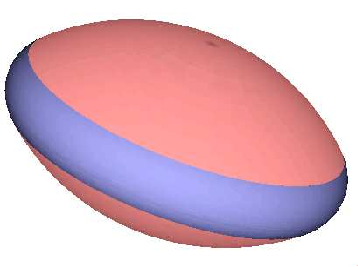
\includegraphics{Figures/snapshot1a}}\quad%
\subfigure[Prolate]
{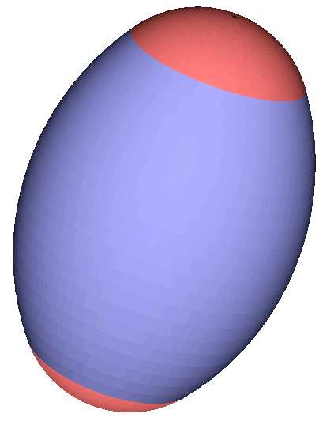
\includegraphics[scale=0.7]{Figures/snapshot1b}}%
\caption{Ovoid particles.}
\label{fig:ovoids}
\end{figure}
%
\item[kshape=6]
nobbies (2D), a non-circular shape that is composed
of clusters of circles (Fig.~\ref{fig:nobbies}).
The particle is neither smooth nor convex.
\begin{figure}
\centering
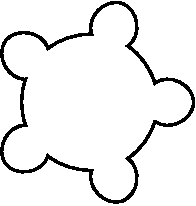
\includegraphics[scale=1.00]{Figures/Nobby_5_03_085}
\caption{Nobby particle: \texttt{nobs=5}, 
                          \texttt{satrad=0.30}, and \texttt{cenrad=0.85}}
\label{fig:nobbies}
\end{figure}
%
\item[kshape=7]
bumpies (3D), a non-spherical shape that is composed
of clusters of spheres (Fig.~\ref{fig:bumpies}).
The particle is neither smooth nor convex.
\begin{figure}
\centering
\subfigure[\texttt{nbumps=2}, \texttt{satrad=0.7}, 
           \texttt{cenrad=0.9}, \texttt{cirrad=0.75}]
{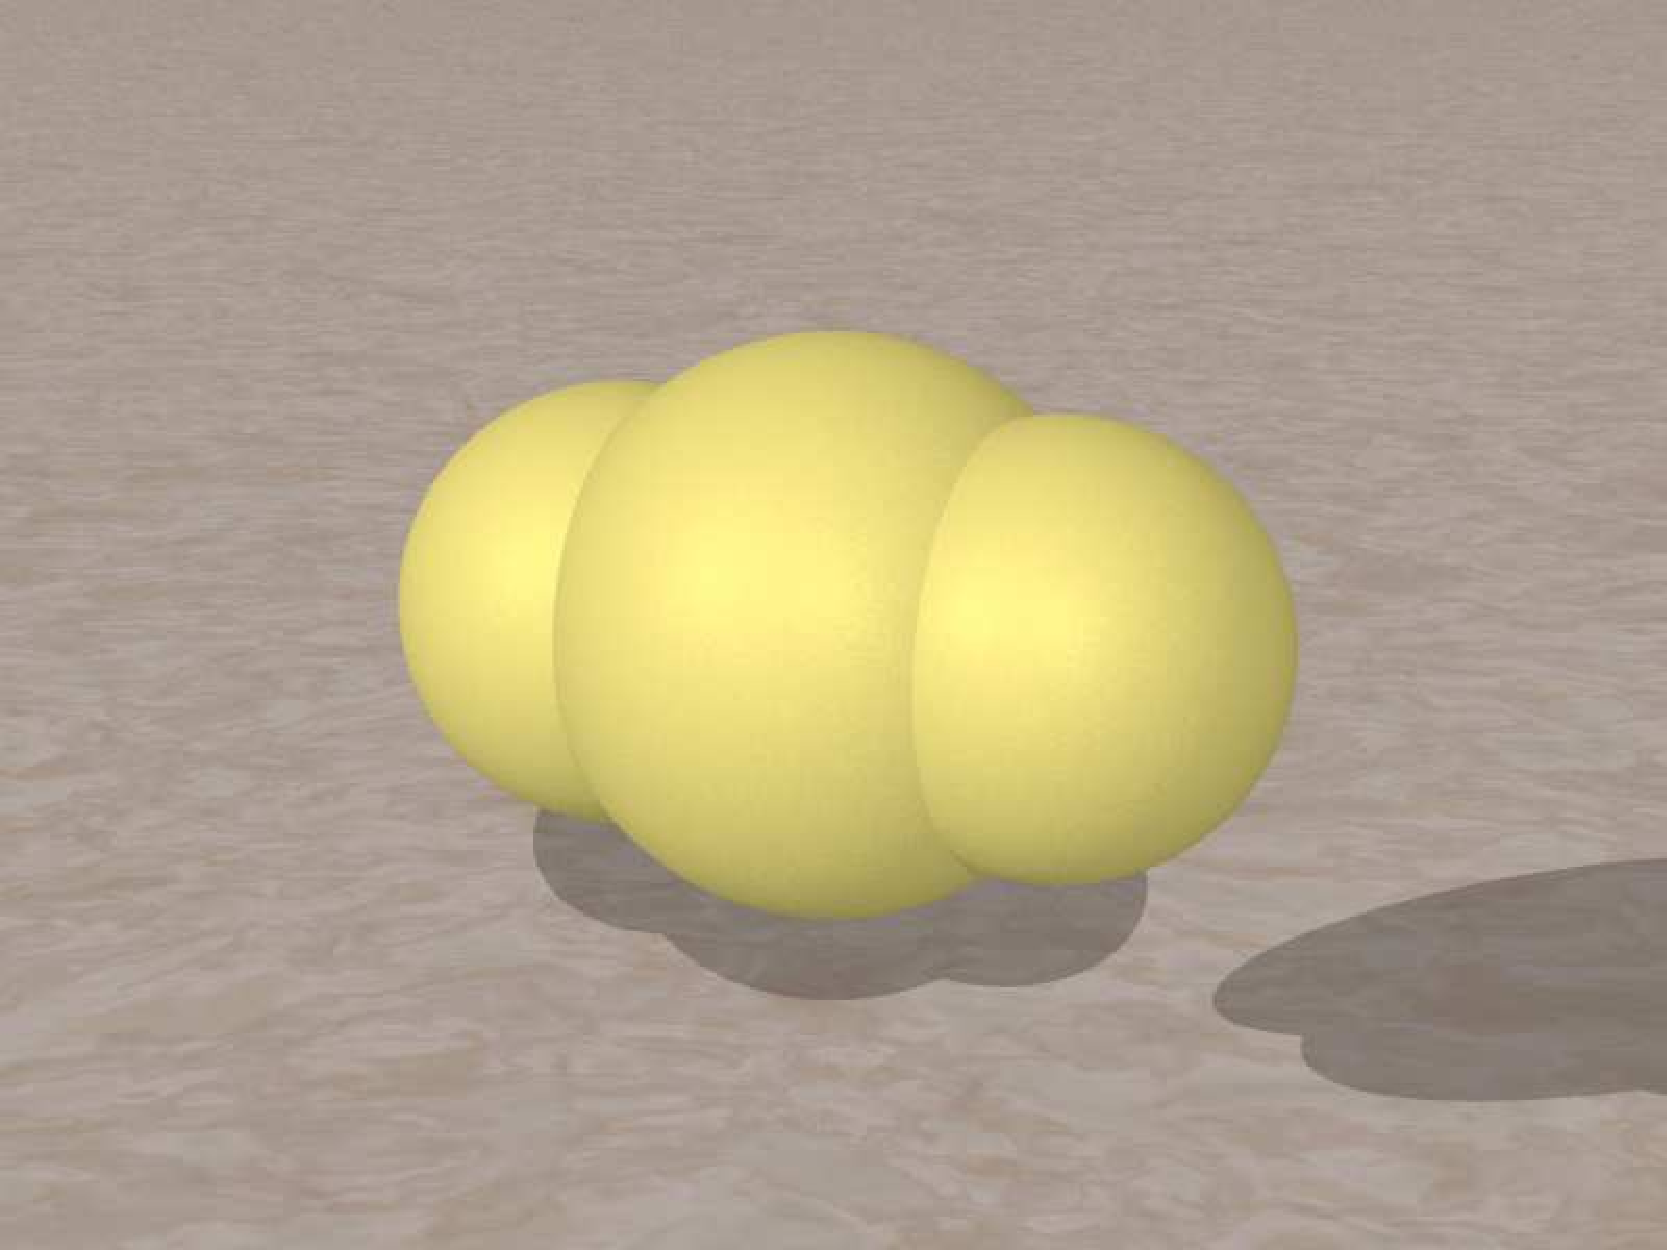
\includegraphics[scale=0.20]{Figures/Bumpy-2-07-09-075-a}}\quad
\subfigure[\texttt{nbumps=3}, \texttt{satrad=0.8}, 
           \texttt{cenrad=1.0}, \texttt{cirrad=0.7}]
{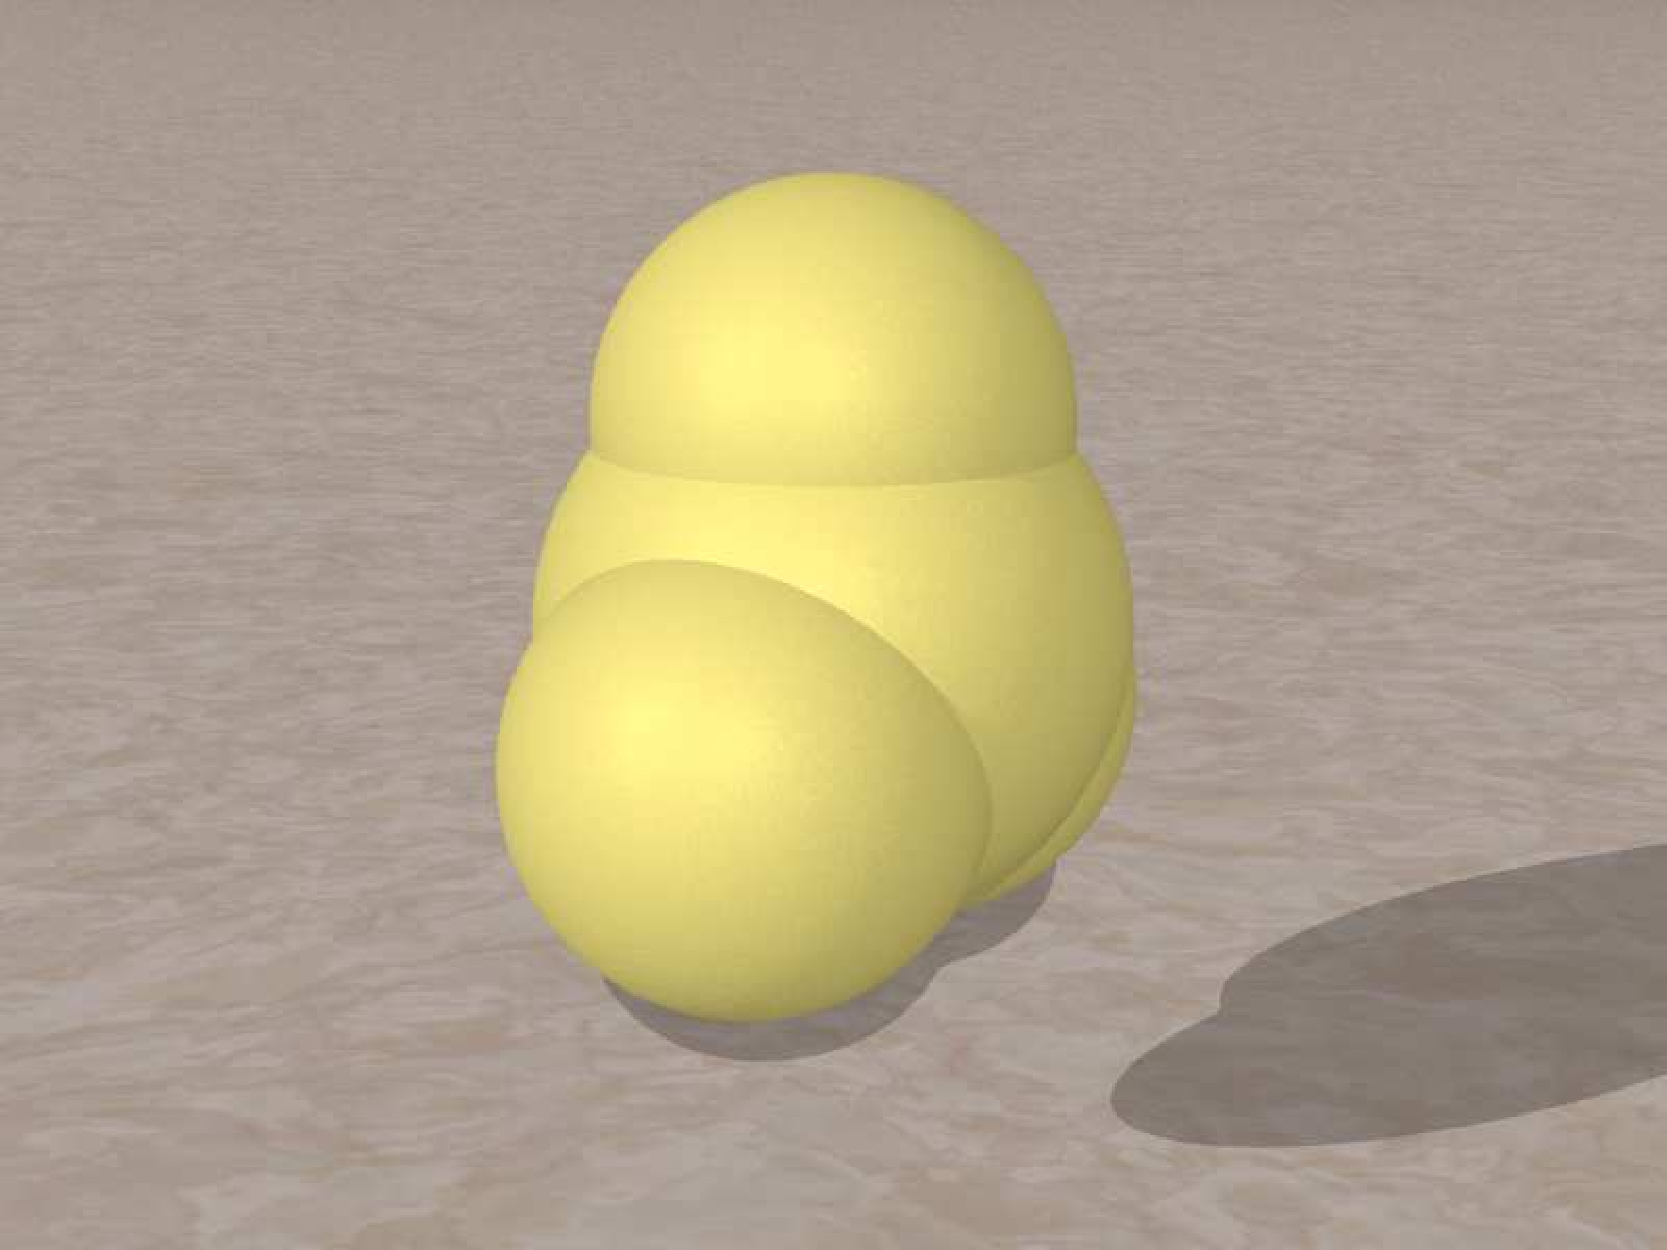
\includegraphics[scale=0.20]{Figures/Bumpy-3-08-10-07-a}}\quad
\subfigure[\texttt{nbumps=4}, \texttt{satrad=0.6},
           \texttt{cenrad=0.8}, \texttt{cirrad=0.7}]
{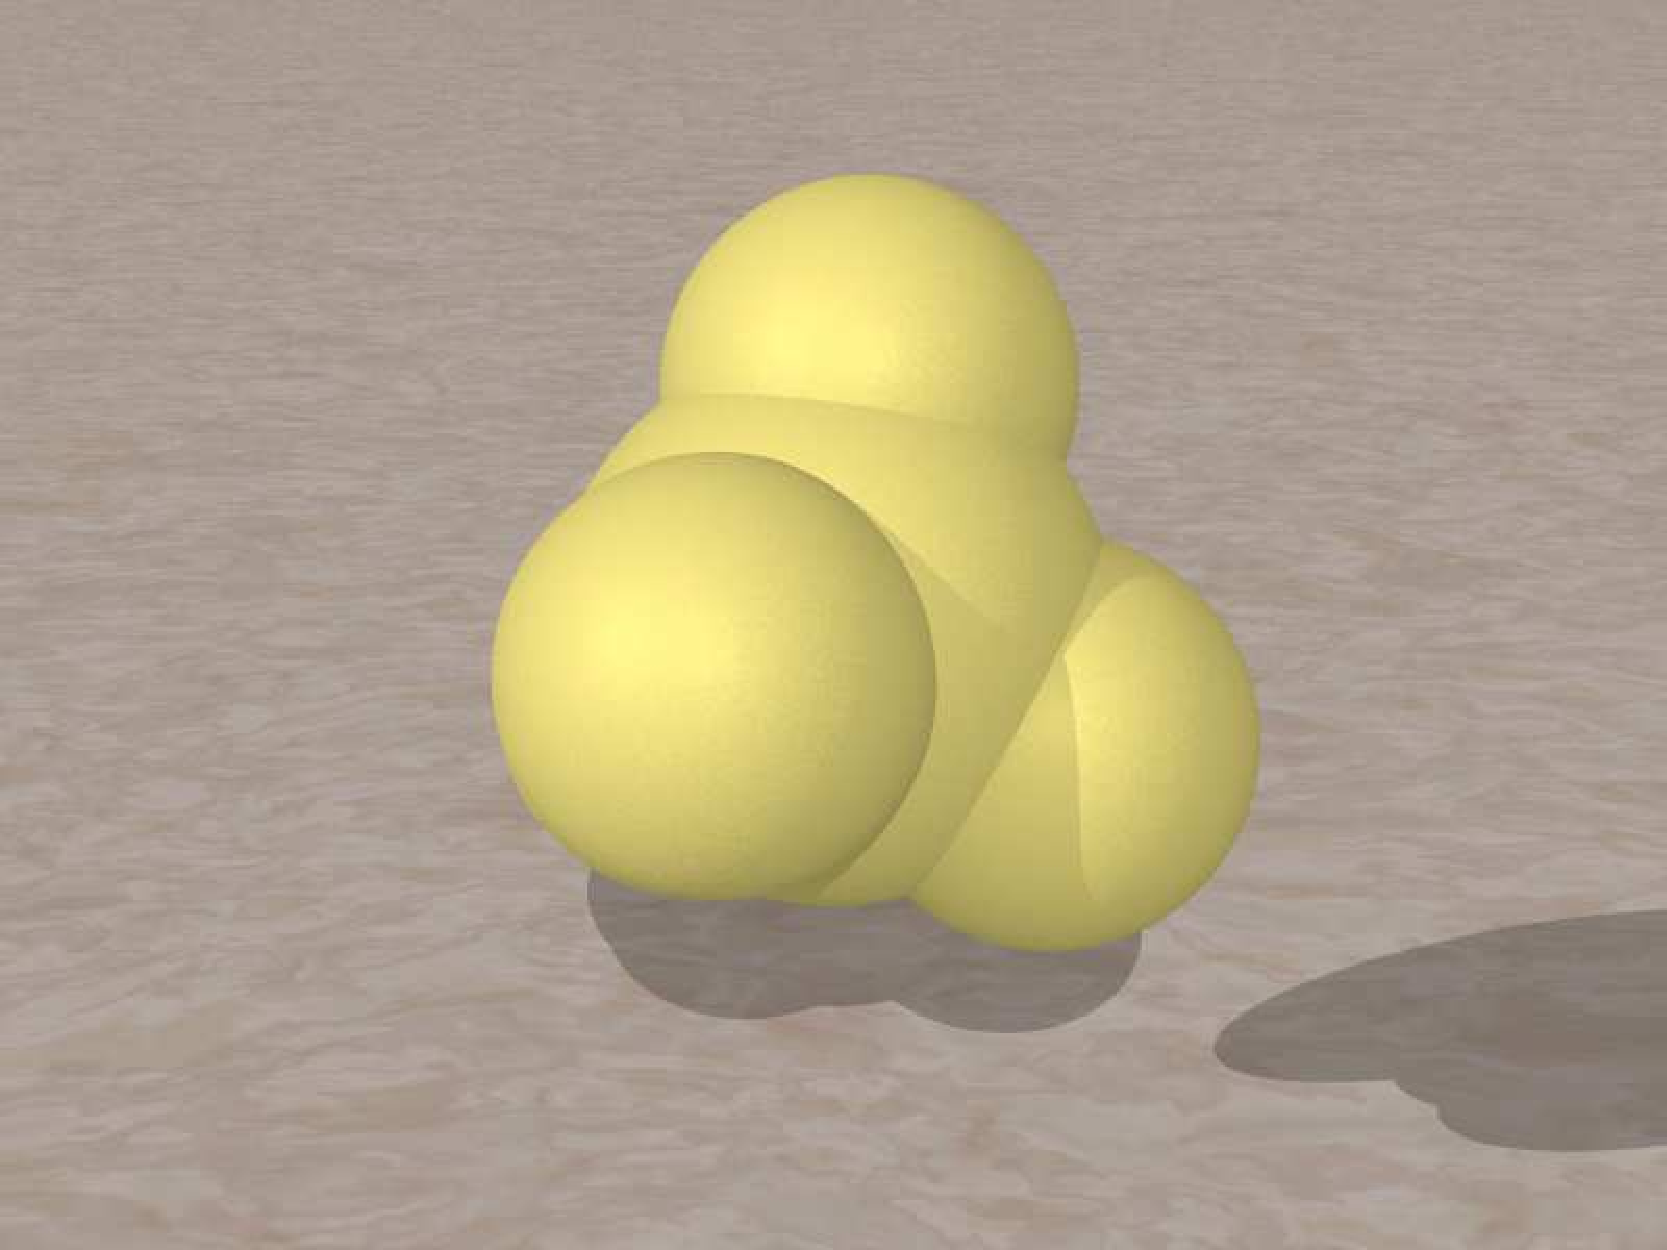
\includegraphics[scale=0.20]{Figures/Bumpy-4-06-08-07-a}}\quad
\subfigure[\texttt{nbumps=6}, \texttt{satrad=0.7},
           \texttt{cenrad=1.0}, \texttt{cirrad=0.6}]
{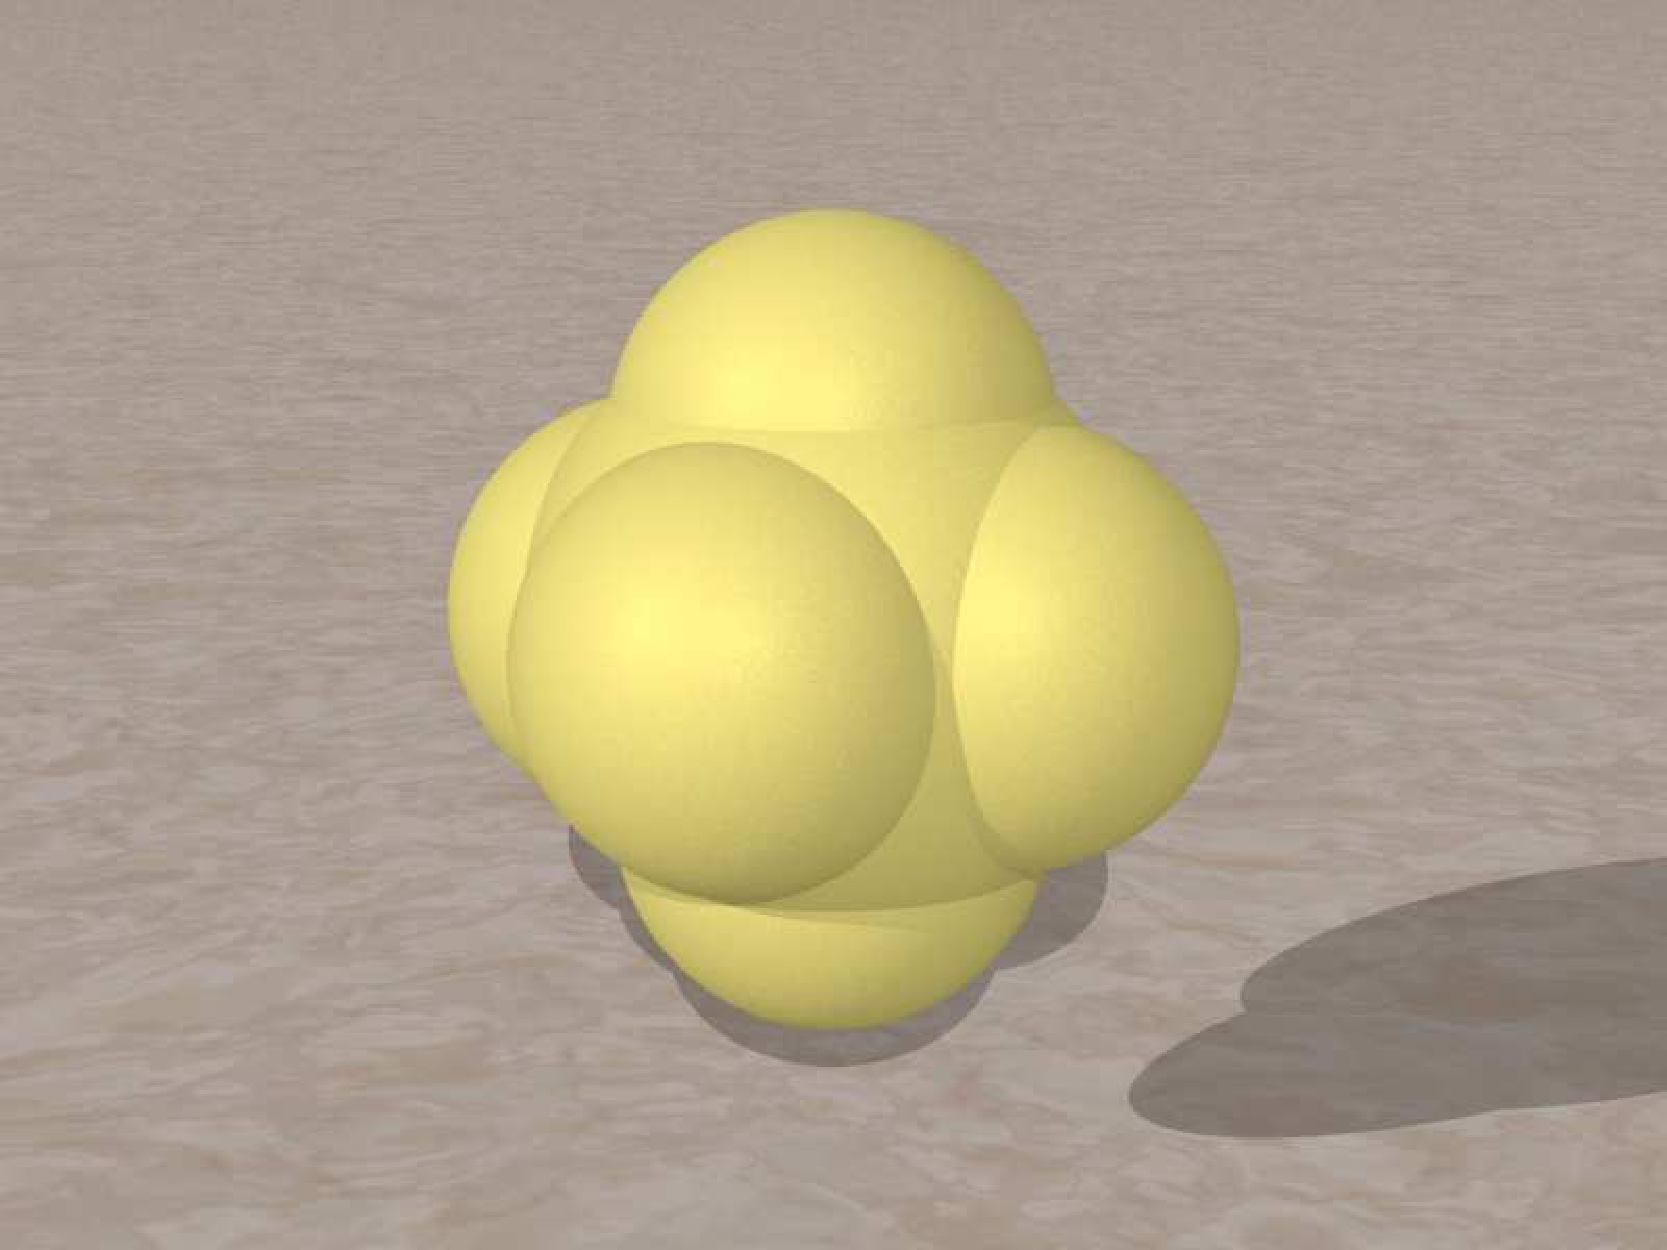
\includegraphics[scale=0.20]{Figures/Bumpy-6-07-10-06-a}}\quad
\subfigure[\texttt{nbumps=8}, \texttt{satrad=0.4},
           \texttt{cenrad=0.9}, \texttt{cirrad=0.8}]
{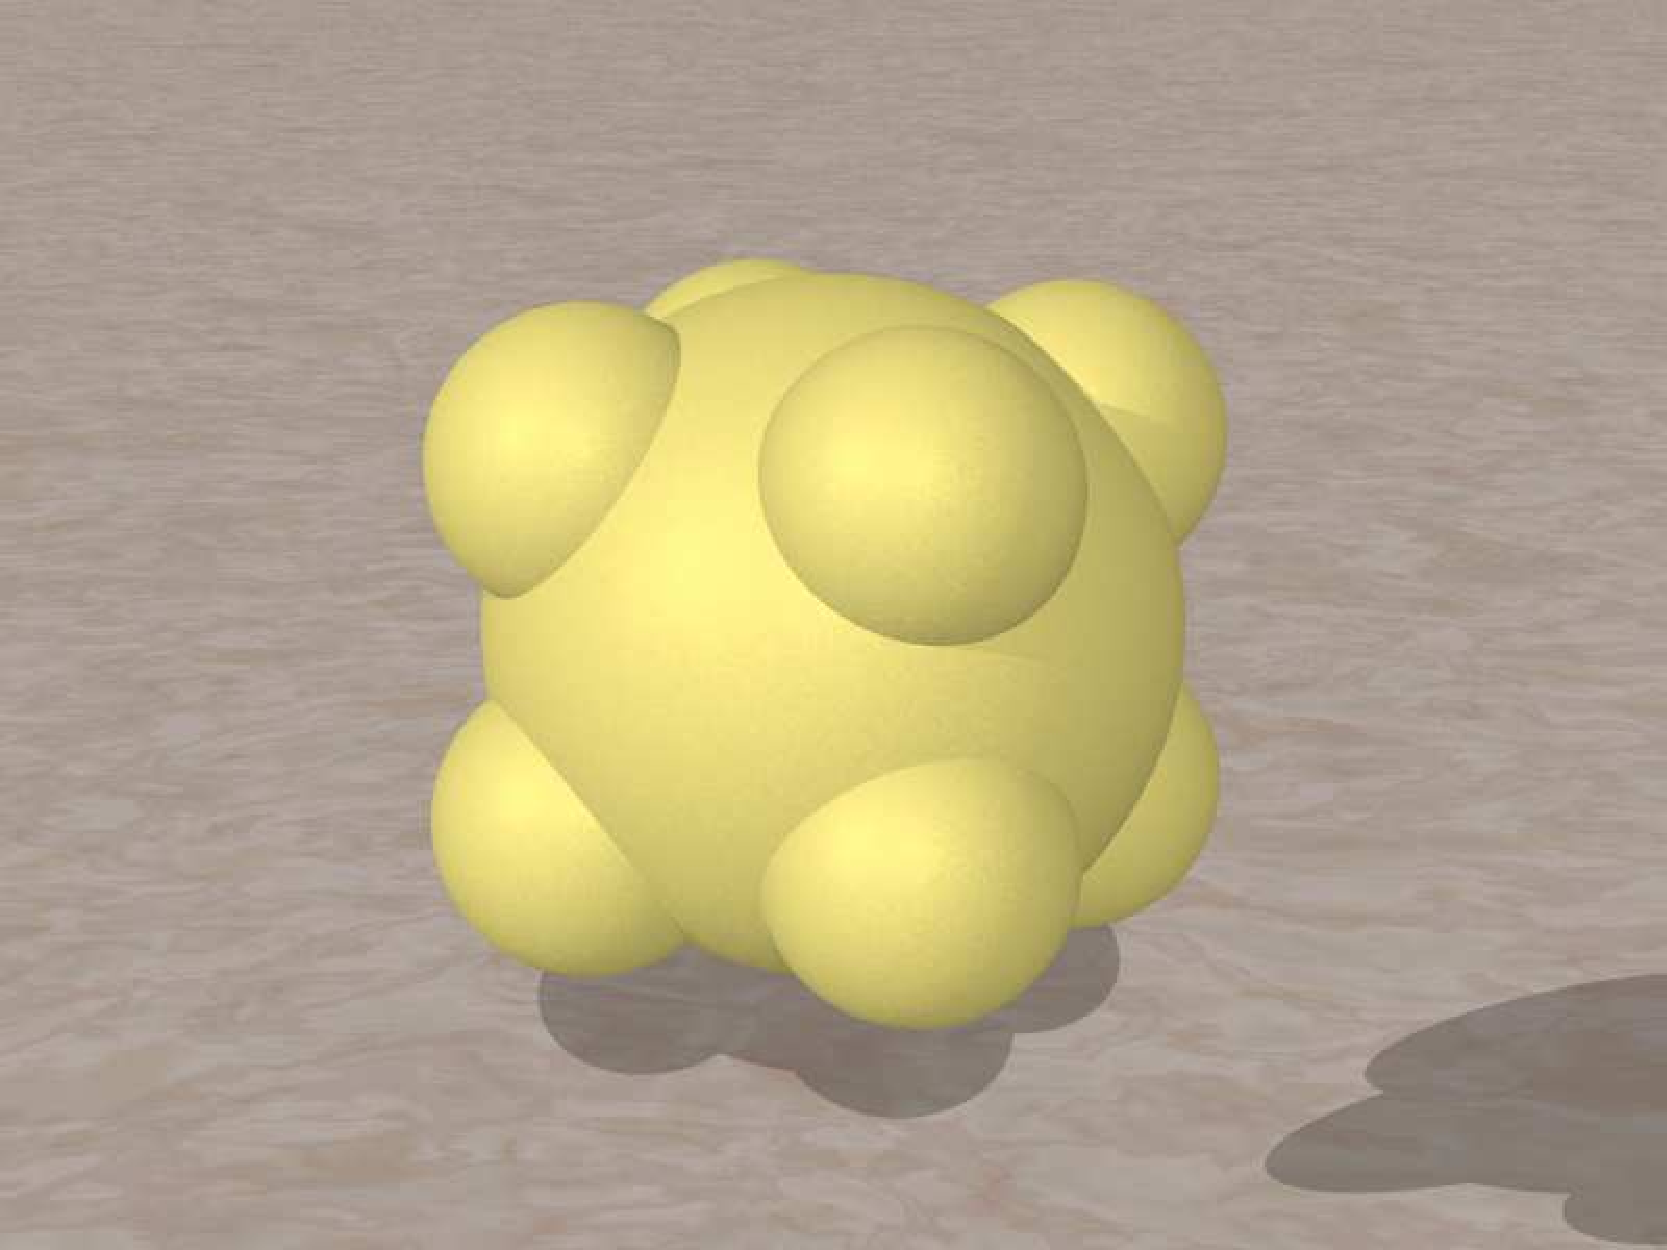
\includegraphics[scale=0.20]{Figures/Bumpy-8-04-09-08-a}}%
\caption{Bumpy particles.}
\label{fig:bumpies}
\end{figure}
\end{Options}
%
\subsubsection[\texttt{np, xcell(1,1)}]{\Var{np,xcell(1,1),xcell(2,2),xcell(3,3)}{i6,3(1pd25.17)}}%
\label{sec:xcell11}
The number of particles, \texttt{np}, 
should appear within the first six columns,
and the three dimensions of the assembly should be presented
in double precision format, with 25 columns per 
dimension (Fig.~\ref{fig:xcells}).
\begin{figure}
  \centering
  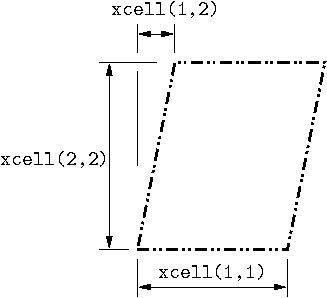
\includegraphics{Figures/xcells.pdf}
  \caption{The \texttt{xcell(i,j)} dimensions for a 2D assembly}
  \label{fig:xcells}
\end{figure}
These dimensions are simply the spacings between opposing periodic
boundaries.
The value of \texttt{xcell(3,3)} must be given, even with
3D assemblies (any value will work, since it will be ignored in the
simulation).
%
\subsubsection[\texttt{xcell(1,2)}]{\Var{xcell(1,2),xcell(1,3),xcell(2,3)}{6x,3(1pd25.17)}}%
\label{sec:xcell12}
After six (blank) columns, the
three shear offsets should be given in double precision format, 
with 25 columns per offset (see the
offset \texttt{xcell(1,2)} in Fig.~\ref{fig:xcells}).
%
\subsubsection[\texttt{beta}]{\Var{beta}{1pd25.17}\ --- oval 
and ovoid particles only!}\label{sec:beta}
When 2D ovals or 3D ovoids are being used, this fourth line contains the
splice angle, \texttt{beta}, in \emph{degrees}
(Fig.~\ref{fig:four_arc}).
\begin{figure}
  \centering
  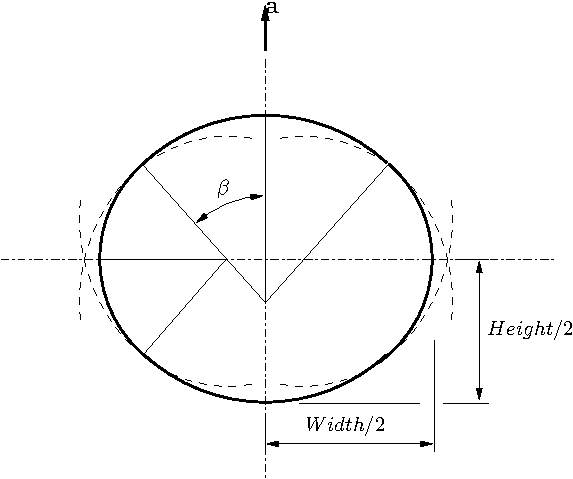
\includegraphics{Figures/four_arc.pdf}
  \caption{Geometry of an oval composed of four circular arcs.}
  \label{fig:four_arc}
\end{figure}
%
The angle $\beta$ must be greater than zero and no greater than $90^{\circ}$.
The particle aspect ratio will be limited by your choice of $\beta$
(Sections~\ref{sec:oval_data} and~\ref{sec:ovoid_data}).
The height/width ratio must lie within the following bounds:
\begin{equation}
\frac{1-\cos\beta}{\sin\beta} < \alpha <%
\frac{\cos\beta}{1-\sin\beta} \;.
\end{equation}
%
\subsubsection[\texttt{nobs} or \texttt{nbumps}]
              {\Var{nobs \textrm{or} nbumps}{* integer}%
              \ --- nobby (2D) and bumpy (3D)
              particles only!}\label{sec:nobs}
When 2D nobby particles are being used, this line contains the
integer number of satellite circles (arcs) that surround a central circle
(see Fig.~\ref{fig:nobbies}).
The input variable \texttt{nobs} gives the integer number of
satellite circles.  These circles are equally spaced around the
central circles.
The satellite circles are centered on a ``circumscribing circle''
of radius $1.0$.
\par
When 3D bumpy particles are being used, this line contains the
integer number of satellite spheres that surround a central sphere
(see Fig.~\ref{fig:bumpies}).
\Oval\ currently restricts \texttt{nbumps} to the following five values:
2, 3, 4, 6, or~8, with examples shown in Fig.~\ref{fig:bumpies}.
In each case, the satellite spheres of a bumpy particles will be centered
on the surface of a ``circumscribing sphere'' (i.e., the
satellite spheres are not necessarily centered on the surface of the
central sphere).
The component spheres of bumpy (3D) particles have the following
arrangements:
%
\begin{Options}
\item[nbumps=2]
Two satellite spheres are place on opposite sides of the central sphere,
diametrically opposed.
The satellite spheres are centered on the surface of a ``circumscribing
sphere.''  See Fig.~\ref{fig:bumpies}a.
\item[nbumps=3]
Three satellite spheres are placed around the central sphere.
The satellite spheres are centered on the vertices of an equilateral triangle
that is circumscribed by the circumscribing sphere.
That is, the satellite spheres are equally spaced along the equator
of the circumscribing sphere.
See Fig.~\ref{fig:bumpies}b.
\item[nbumps=4]
Four satellite spheres are placed around the central sphere.
The satellite spheres are centered on the vertices of a
tetrahedron that is circumscribed by the circumscribing sphere.
That is, the satellite spheres are equally spaced around the full surface
of the circumscribing sphere.
See Fig.~\ref{fig:bumpies}c.
\item[nbumps=6]
Six satellite spheres are placed around the central sphere.
The satellite spheres are centered on the vertices of a
octahedron that is circumscribed by the circumscribing sphere.
That is, the satellite spheres are equally spaced around the full surface
of the circumscribing sphere.
See Fig.~\ref{fig:bumpies}d.
\item[nbumps=8]
Eight satellite spheres are placed around the central sphere.
The satellite spheres are centered on the vertices of a
cube that is circumscribed by the circumscribing sphere.
That is, the satellite spheres are equally spaced around the full surface
of the circumscribing sphere.
See Fig.~\ref{fig:bumpies}e.
\end{Options}
\par
Regardless of whether nobbies or bumpies are being used, 
this line of input must be followed by a line
that gives relative sizes of the circles or spheres that comprise
a particle, as in the
following section (Section~\ref{sec:satrad}).

\subsubsection[\texttt{satrad}, \texttt{cenrad}, \texttt{cirrad}]
              {\Var{satrad, cenrad, cirrad}{* double precision}\ --- nobby 
              (2D) bumpy and (3D) particles only!}\label{sec:satrad}
These values are only used with nobby (2D) bumpy (3D) particles, and
they are placed on a single line in double-precision format separated with
spaces.
\par
Every particle in an assembly will have the same shape, but they
can have different sizes.  
Their common shape is specified with the values of \texttt{nobs},
\texttt{nbumps}, \texttt{satrad}, \texttt{cenrad}, and \texttt{cirrad}.
These values give a ``base'' shape and size for the particles.
The actual size of each particle is equal to the common ``base size''
multiplied by an individual scaling radius for each particle
(Sections~\ref{sec:nobby_data} and~\ref{sec:bumpy_data}).
\par
The input variables \texttt{satrad} and \texttt{cenrad} are the
base sizes of the satellite and central circles or spheres of the 
nobby~(2D) and bumpy~(3D) cluster particles.
The input variable \texttt{cirrad} is the radius of circumscribing
sphere, as described in Section~\ref{sec:nobs}.
\Oval\ currently does not support \texttt{cirrad} for 2D nobby particles:
the satellite circles are centered on a circumscribing circle
of radius $1.0$.
%
\subsection{Particle data in \texttt{D}-\textsf{StartFiles}}%
\label{sec:StartFile2}
Following the general information at the head of a 
\texttt{D}\textsf{StartFile}, information is given on each particle,
with one line per particle.  
The arrangement of this data depends upon the type
of particle.
\subsubsection{Circle particle data}\label{sec:circle_data}
Three fields give the radius,
the $x_{1}$--location, and the $x_{2}$--location of the particle.
The location coordinates refer to the center of the particle.
Following the general information at the head of a
\texttt{D}\textsf{StartFile}, this
information is given for each circle,
with each circle beginning on a new line.
The data items are listed below.
Each data field is in \texttt{1pd25.17} format, with
spaces or a new line between the fields.
In \Oval\ versions 0.6.0 and higher, 
the data can be provided in \emph{free format},
so that data fields do \emph{not} have to be aligned 
within certain columns.
The example input on page~\pageref{page:dfile}
shows two lines of data for circular particles.
\begin{itemize}
\item
Radius of the circle.
\item
$x_{1}$--location of the circle's center.
\item
$x_{2}$--location of the circle's center.
\end{itemize}
\subsubsection{Oval particle data}\label{sec:oval_data}
Five fields give the oval width, the ratio of height divided
by the width,
the $x_{1}$--location, the $x_{2}$--location, and the orientation
angle (in \emph{degrees}) of particle, measured counterclockwise
from the $x_{1}$-direction (Fig.~\ref{fig:orientation_angle}).
%
\begin{figure}
  \centering
  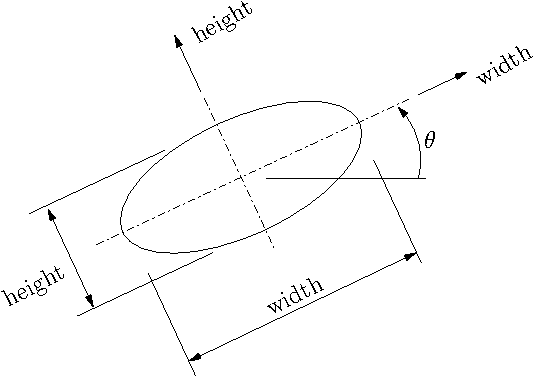
\includegraphics{Figures/orientation.pdf}
  \caption{Orientation angle $\theta$ for elongated particles (2D ovals
           and ellipses).}
  \label{fig:orientation_angle}
\end{figure}
%
The location coordinates refer to the center of the particle.
Following the general information at the head of a
\texttt{D}\textsf{StartFile}, this
information is given for each oval,
with each oval beginning on a new line.
The data items are listed below.
Each data item is given in \texttt{1pd25.17} format, with
spaces or a new line between the fields.
In \Oval0.6.0, the data can be provided in \emph{free format},
so that data fields do \emph{not} have to be aligned
within certain columns.
\begin{itemize}
\item
Half-width of the oval.  
Note that the oval width may be greater or less than the height
(with ellipses, the width must be greater than its height).  
The width is measured as shown in 
(Fig.~\ref{fig:orientation_angle}), at an angle of $\theta$ counterclockwise
from the horizontal $x_{1}$ axis.
As input, you should give one half of the full particle width.
\item
Ratio of the height divided by the width of the particle
(Fig.~\ref{fig:orientation_angle}).  
For ovals, the ratio may be greater or less than one.
\item
$x_{1}$--location of the oval's center.
\item
$x_{2}$--location of the oval's center.
\item
Orientation angle $\theta$
of the oval's width (in degrees, Fig.~\ref{fig:orientation_angle}).
\end{itemize}
%
\subsubsection{Ellipse particle data}\label{sec:ellipse_data}
The code for this has not been recently tested
and might not be stable.
Five fields give the major radius, the ratio of the minor radius
divided by the major radius (a number greater than zero, but
no greater than one),
the $x_{1}$-location, the $x_{2}$-location, and the orientation
angle (in \emph{degrees}) of the major axis, measured counterclockwise
from the $x_{1}$-direction (Fig.~\ref{fig:orientation_angle}).
The location coordinates refer to the center of the ellipse.
Following the general information at the head of a
\texttt{D}\textsf{StartFile}, this
information is given for each ellipse,
with each ellipse beginning on a new line.
The data items are listed below.
Each data item is given in \texttt{1pd25.17} format, with
spaces or a new line between the fields.
In \Oval0.6.0, the data can be provided in \emph{free format},
so that data fields do \emph{not} have to be aligned
within certain columns.
At present, the ellipse width must be greater than its height, with
a height-to-width ratio less than one.
\begin{itemize}
\item
Major radius of the ellipse.
\item
Ratio of the minor radius divided by the major radius of the particle
(Fig.~\ref{fig:orientation_angle}).
For ellipses, the ratio must be greater than zero, but no greater than one.
\item
$x_{1}$--location of the ellipse's center.
\item
$x_{2}$--location of the ellipse's center.
\item
Orientation angle $\theta$ of the ellipse's width (in degrees, Fig.~\ref{fig:orientation_angle}).
\end{itemize}
%
\subsubsection{Sphere particle data}\label{sec:sphere_data}
Four fields give the radius,
the $x_{1}$--location, the $x_{2}$--location, and the $x_{3}$--location 
of the particle.
The location coordinates refer to the center of the particle.
Following the general information at the head of a
\texttt{D}\textsf{StartFile}, this
information is given for each sphere,
with each sphere beginning on a new line.
The data items are listed below.
Each data item is given in \texttt{1pd25.17} format, with
spaces or a new line between the fields.
In \Oval0.6.0, the data can be provided in \emph{free format},
so that data fields do \emph{not} have to be aligned
within certain columns.
\begin{itemize}
\item
Radius of the sphere.
\item
$x_{1}$--location of the sphere's center.
\item
$x_{2}$--location of the sphere's center.
\item
$x_{3}$--location of the sphere's center.
\end{itemize}
%
\subsubsection{Ovoid particle data}\label{sec:ovoid_data}
Seven fields give the
ovoid's revolved radius, the ratio of the axial radius divided
by the revolved radius, the location coordinates, and the orientation
angles $\gamma_{1}$ and $\gamma_{2}$ of the ovoid's axis of revolution,
$\mathbf{a}$.
An ovoid is formed by rotating an oval (i.e. Fig.~\ref{fig:four_arc})
about its central axis $\mathbf{a}$.
The location coordinates refer to the center of the particle.
Following the general information at the head of a
\texttt{D}\textsf{StartFile}, this
information is given for each ovoid,
with each ovoid beginning on a new line.
The data items are listed below.
Each data item is given in \texttt{1pd25.17} format, with
spaces or a new line between the fields.
In \Oval0.6.0, the data can be provided in \emph{free format},
so that data fields do \emph{not} have to be aligned
within certain columns.
\begin{itemize}
\item
Half of the transverse (revolved, half) width of the ovoid.  
This half-width is measured perpendicular
to the central axis of revolution, $\mathbf{a}$.
\item
Ratio of the axial height divided
by the transverse width.  
The ratio can be greater or less than one, but it must be greater than zero.
Ratios less than one are oblate; ratios greater than one are prolate
(Fig.~\ref{fig:ovoids}).
Note that large aspect ratios (or small inverse ratios) require much more
computation time.  I would not recommend using a ratio greater than 2 or
less than 0.5.
\item
$x_{1}$--location of the ovoid's center.
\item
$x_{2}$--location of the ovoid's center.
\item
$x_{3}$--location of the ovoid's center.
\item
$\gamma_{1}$ orientation angle (in radians) of the ovoid's axis
of revolution, $\mathbf{a}$ (Fig.~\ref{fig:coordinates}).  
This angle should be no less than zero and no greater than
90$^{\circ}$.
\begin{figure}
  \centering
  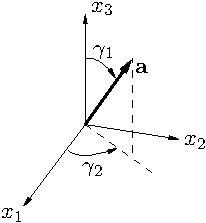
\includegraphics{Figures/coordinates}
  \caption{Orientation angles $\gamma_{1}$ and $\gamma_{2}$ 
           for 3D ovoid particles.
           Vector $\mathbf{a}$ is the central axis of revolution of the ovoid
           (Figs.~\ref{fig:four_arc} and~\ref{fig:orientation_angle}).}
  \label{fig:coordinates}
\end{figure}
\item
$\gamma_{2}$ orientation angle (in radians) of the ovoid's axis
of revolution $\mathbf{a}$ (Fig.~\ref{fig:coordinates}).
\end{itemize}
%
%
\subsubsection{Nobby (2D) particle data}\label{sec:nobby_data}
Four fields give the scaling radius, 
the $x_{1}$--location, the $x_{2}$--location, and the orientation
angle (in degrees) of the particle.
The location coordinates refer to the center of the particle.
Following the general information at the head of a
\texttt{D}\textsf{StartFile}, this
information is given for each nobby,
with each nobby beginning on a new line.
The data items are listed below.
Each data item is given in \texttt{1pd25.17} format, with
spaces or a new line between the fields.
In \Oval0.6.0, the data can be provided in \emph{free format},
so that data fields do \emph{not} have to be aligned
within certain columns.
\begin{itemize}
\item
Scaling radius of the nobby particle.
This scaling radius is multiplied by the base radii,
\texttt{satrad} and \texttt{cenrad}, as described
in Section~\ref{sec:satrad}.
These products give the actual sizes of the radii that comprise
the nobby particle.
\item
$x_{1}$--location of the nobby particle's center.
\item
$x_{2}$--location of the nobby particle's center.
\item
$\theta_{3}$ orientation angle (in degrees) of the particle.
The center of one of the satellite particles is located at
angle $\theta_{3}$, measured counter-clockwise from the $x_{1}$--direction.
The other satellite circles are equally spaced at angle
\mbox{$360^{\circ}/$\texttt{nobs}}.
\end{itemize}
%
%
\subsubsection{Bumpy (3D) particle data}\label{sec:bumpy_data}
Eight fields give the scaling radius, 
the $x_{1}$--location, the $x_{2}$--location, 
the $x_{3}$--location, and a four-component unit quaternion
of the particle's orientation.
The location coordinates refer to the center of the particle.
Following the general information at the head of a
\texttt{D}\textsf{StartFile}, this
information is given for each bumpy,
with each bumpy beginning on a new line.
The data items are listed below.
Each data item is given in \texttt{1pd25.17} format, with
spaces or a new line between the fields.
In \Oval0.6.0, the data can be provided in \emph{free format},
so that data fields do \emph{not} have to be aligned
within certain columns.
\begin{itemize}
\item
Scaling radius of the bumpy particle.
This scaling radius is multiplied by the base radii
(\texttt{satrad}, \texttt{cenrad}, and \texttt{cirrad}) as described
in Section~\ref{sec:satrad}.
These products give the actual sizes of the radii that comprise
the nobby particle.
\item
$x_{1}$--location of the nobby particle's center.
\item
$x_{2}$--location of the nobby particle's center.
\item
$x_{3}$--location of the nobby particle's center.
\item
$\mathtt{Qp}_{1}$ orientation quaternion of the particle.
\item
$\mathtt{Qp}_{2}$ orientation quaternion of the particle.
\item
$\mathtt{Qp}_{3}$ orientation quaternion of the particle.
\item
$\mathtt{Qp}_{4}$ orientation quaternion of the particle.
\end{itemize}
%
%
\section{Text output files from \Oval}\label{sec:MacroOutput}
While \Oval\ is running,
output is periodically written to two files:
an A-file and a B-file.
The frequency at which this occurs is specified with the input variable
\texttt{ipts} (Section~\ref{sec:ipts}).
These two files contain macro-data, such as stress and
deformation.
A-files and B-files are described in 
Sections~\ref{sec:Afiles}--\ref{sec:bfiles3d}.
You can also produce F-files, which will contain micro-level data.
Because F-files can be quite large, each creation of these files must
be triggered by the input value \texttt{imicro} in the
\RunFile\ (Section~\ref{sec:imicro}).
F-files are described in Sections~\ref{sec:ffiles}--\ref{sec:ffiles3d}.
%
\subsection{A-files: macro-data for spreadsheets}\label{sec:Afiles}
A simulation will create a file named 
\texttt{A<}\textsf{RunFile}\texttt{>.txt}, which 
will be referred to as simply an ``A-file''.
The fields in this text file are separated by Tab characters, 
so that A-files can
be imported into a spreadsheet (note: \emph{imported} not opened).
When importing, you will want to specify the columns as being "tab separated."
The spreadsheet is headed with some general information about the simulation,
followed by a history of time, strains, and stresses.
The strains are reported with the simple measure
\begin{equation}\label{eq:strain}
F_{ij} - \delta_{ij}
\end{equation}
where $F_{ij}$ are components of the deformation gradient tensor.
Note that the shear deformations are reported as shear angles,
like $F_{12}$, or 
twice the shear strain (a $\gamma$-strain, not an $\varepsilon$-strain).
Stresses and strains are reported at the interval
\texttt{ipts},
which may differ for each segment
of the deformation-stress path 
(Sections~\ref{sec:runfile2} and~\ref{sec:ipts}).
%
\par
For 2D assemblies, the A-file includes information on the assembly's
particle graph \cite{Satake:1992a,Satake:1993b,Kuhn:1999a}.
This information includes the numbers of vertices (particles that are included
in the particle graph), edges (contacts between particles),
and face (void cells).
\par
For both 2D and 3D assemblies, the A-file includes information on
the \emph{fabric tensor} for the assembly \cite{Satake:1982a}.
We will refer to the fabric tensor with the symbol $\mathbf{A}$, which
is defined with a sum over contacts 
within the assembly.  Note that in an A-file, this tensor
$\mathbf{A}$ is unfortunately labeled as ``\texttt{F}'', with the components
\texttt{F(1,1)}, \texttt{F(2,2)}, etc.
\begin{equation}\label{eq:fabric1}
A_{ij} = \frac{1}{N}
\sum_{k=1}^{N}
n_{i}^{k} n_{j}^{k}\;,
\end{equation}
where $\mathbf{n}^{k}$ is the (unit vector) direction of the 
$k$th branch vector (contact),
and $N$ is the number of contacts in the assembly.
When computing~(\ref{eq:fabric1}), $N$ includes only
those contacts between particles that each have at least 2 contacts
(2D assemblies) or 3 contacts (3D assemblies).
\par
For both 2D and 3D assemblies, the A-file also includes information
on the fabric tensor $\mathbf{A}^{s}$ of only those (``strong'') contacts that
carry a greater-than-average force.
Note that in an A-file, this tensor
$\mathbf{A}$ is unfortunately labeled as ``\texttt{Fs}'', with the components
\texttt{Fs(1,1)}, \texttt{Fs(2,2)}, etc.
This tensor is defined as a sum over the strong contacts within
the assembly:
\begin{equation}\label{eq:fabric2}
A_{ij}^{s} = \frac{1}{N}
\sum_{k\in \mathcal{S}}
n_{i}^{k} n_{j}^{k}\;,
\end{equation}
Where the set of contacts $\mathcal{S}$ is a set of contacts $k$:
\begin{equation}
\mathcal{S} = \{k: |\mathbf{f}^{k}| > \overline{f} \}
\end{equation}
that have a force magnitude $|\mathbf{f}^{k}|$ greater than average:
\begin{equation}
\overline{f} = \sqrt{
\frac{\sum_{k=1}^{N} |\mathbf{f}^{k}|^{2}} {N}
                    }
\end{equation}
The A-file also report the proportion $v$ of strong contacts in the assembly.
\par
An A-file contains several more columns of data.  The labels of these
columns explain their content, and many are given the same names as
quantities that are described below for B-files (Section~\ref{sec:Bfiles}).
%
\subsection{B-files: macro-data text files}\label{sec:Bfiles}
The \texttt{B<}\textsf{RunFile}\texttt{>} (or just ``B''-files)
contain more information than A-files---not only 
stresses and deformations, but information
that reflects the numerical performance of the simulation.
For example, the B-file contains information that can characterize
whether the simulation was nearly pseudo-static
(\texttt{chi1}, \texttt{chi2}, \texttt{chi3}, \texttt{chi4}, and
\texttt{knrgy}), 
the relative importance
of viscous damping during the simulation
(\texttt{chi3}, \texttt{chi4}, \texttt{viscbt}, and \texttt{viscct}),
and whether the controlled stresses
were maintained near their target values (\texttt{psi}).
This information, although useful, is packed into a text (ASCII) file
that can be somewhat difficult to read and understand.
B-files are described in the following two sections.
%
\subsection{B-files with 2D simulations}\label{sec:bfile2d}
The first line in the B-file contains the following 
three pieces of information in \texttt{format(i4,2x,a50,2x,a20)}:
\begin{itemize}
\item
an integer that indicates the format of the B-file,
\item
the name of the \textsf{StartFile} that was used for the simulation
(Sections~\ref{sec:RunOval} and~\ref{sec:startfileD}), and
\item
the version of the \Oval\ source code.
\end{itemize}
This line is followed by the results of each output cycle,
which occur
at the frequency \texttt{ipts} (see Section~\ref{sec:ipts}).
For 2D simulations, the information for each output cycle is packed
into just three lines, such as the following:
\par\noindent
\footnotesize\normalfont
\begin{verbatim}
1.0320000E-04   5.948067E-05 -1.984000E-04  0.000000E+00  4.212188E-04     1623
  6.49E-04     -1.551593E+04 -2.071540E+04 -2.774535E+01  9.690910E+00 3.29E-07
  1.03E-03 0.00E+00 7.11E-04  6.519467E-03  5.346882E-02  2.655151E+00     3.00
\end{verbatim}
\normalsize\normalfont
\par
The contents of these three lines
correspond to the following variables (some of these
are, in fact, arrays):
\footnotesize\normalfont
\begin{verbatim}
  timer         defout(1,1)   defout(2,2)   defout(1,2)    knrgy         ntacts
   chi1         stress(1,1)   stress(2,2)   stress(1,2)    pnrgy           psi 
   chi2    chi3     chi4      viscbt        slidet         work1t        xloops
\end{verbatim}
\normalsize\normalfont
and in the following formats:
\footnotesize\normalfont
\begin{verbatim}
 1pe14.7,   1x,  1pe14.6,     1pe14.6,      1pe14.6,       1pe14.6,       i9,/,
 2x,1pe9.2, 4x,  1pe14.6,     1pe14.6,      1pe14.6,       1pe14.6,   1pe9.2,/,
 2x,1pe9.2, 1pe9.2, 1pe9.2,   1pe14.6,      1pe14.6,       1pe14.6,   0pf9.2
\end{verbatim}
\normalsize\normalfont
The various output values are now described.
%
\subsubsection{\texttt{timer}}
The accumulated time, which advances by an amount \texttt{dt} with each
deformation step (Section~\ref{sec:dt}).
%
\subsubsection{\texttt{defout(i,j)}}\label{sec:defout}
The output values, \texttt{defout(i,j)}, are the difference
between the deformation gradient matrix $F_{ij}$ and the
identity (Kronecker) matrix $\delta_{ij}$, as in eqn~\ref{eq:strain} on
page~\pageref{eq:strain}.
For example, the output
\begin{verbatim}
     defout(1,1) =  0.001
     defout(2,2) = -0.002
     defout(1,2) =  0.003
\end{verbatim}
for a 2D assembly corresponds to the following deformation gradient:
\begin{equation}
\mathbf{F} = \left[
\begin{array}{cc}
1.001 & 0.003\\
0     & 0.998
\end{array}
\right]
\end{equation}
The deformation gradient $\mathbf{F}$ is referenced to the initial
assembly (except when the simulation is started with
a C-\StartFile, in which case, $\mathbf{F}$ is carried over
from a previous run).
%
\subsubsection{\texttt{knrgy}}
The kinetic energy of particle motions per unit of the assembly's 
original volume.  
The kinetic energy is computed from both 
translational and rotational velocities of the particles:
\begin{equation}
\frac{1}{\mathrm{Initial\ volume}}
\times
\frac{1}{2}
\sum_{\text{Particles}} \left(
m \bar{\mathbf{v}}^{2} + I \bar{\boldsymbol{\omega}}^{2}
\right)\;,
\end{equation}
where $m$ and $I$ are the mass and the mass moment of inertia of a particle, 
and $\bar{\mathbf{v}}$ and $\bar{\boldsymbol{\omega}}$ are the
average velocity and angular velocity of a particle 
(the averages of the velocities at the two times
$t-dt/2$ and $t+dt/2$).
The energy \texttt{knrgy} is not really meaningful
when \texttt{algori=2} (see Sections~\ref{sec:algori}.
Note that $F_{ij}=0$ for $i>j$, as is the case
in Fig.~\ref{fig:xcells}.
%
\subsubsection{\texttt{ntacts}}
The number of contacts.  Here, a contact is shared by two particles.  If you
prefer to count a contact twice (once for each of the two particles,
as in Table~\ref{table:assemblies}), then
the number of contacts is, instead, \texttt{ntacts}$\times2$.
%
\subsubsection{\texttt{chi1}}\label{sec:chi1}
One of four measures for determining whether the simulation is nearly
pseudo-static.
The property \texttt{chi1} is the average force imbalance on a particle
divided by the average magnitude of a contact force.
Small values signify that the particles were nearly in equilibrium 
during the deformation process.
When \texttt{algori=2},
the variables \texttt{chi1} and \texttt{chi2} (Section~\ref{sec:chi2})
are used as a near-equilibrium criteria
for controlling the pace at which the deformation is allowed to proceed
(Sections~\ref{sec:algori} and~\ref{sec:xloops}).
If there are no contacts within the assembly, then \texttt{chi1} will be zero.
%
\subsubsection{\texttt{stress(i,j)}}
Components of the Cauchy stress tensor.
%
\subsubsection{\texttt{pnrgy}}
The elastic energy stored in the contact springs per unit of the assembly's
original volume.
For the simple linear contact mechanism,
this energy is calculated as
\begin{equation}
\frac{1}{\mathrm{Initial\ volume}}
\times
\frac{1}{2}
\sum_{\text{Contacts}} \left[
\frac{f_{n}^{2}}{k_{n}}
+
\frac{f_{t}^{2}}{k_{t}}
\right]\;,
\end{equation}
where $f_{n}$ and $f_{t}$ are the normal and tangential contact forces,
and $k_{n}$ and $k_{t}$ are the normal and tangential contact
stiffnesses at time $t$.
%
\subsubsection{\texttt{psi}}\label{sec:psi}
This performance measure
characterizes the fluctuation of the controlled stresses from
their intended (target) values. 
When one or more digits in \texttt{icontr} are \texttt{1}'s, then
a servo-control algorithm will attempt
to control certain components of the Cauchy stress 
and maintain them at target values (see Section~\ref{sec:icontr}).
The property \texttt{psi} is the sum of the deviations of the controlled
stress components from their
target values divided by the mean stress
(either $1/2$ or $1/3$ $\sigma_{kk}$).
If you are not controlling any of the stress components, then \texttt{psi}
will be zero.
%
\subsubsection{\texttt{chi2}}\label{sec:chi2}
This is another measure of whether the simulation is nearly
pseudo-static (see \texttt{chi1}, Section~\ref{sec:chi1}).
The value \texttt{chi2} is the average \emph{moment} imbalance on a 
particle divided by both the average magnitude of a contact force and the
average particle radius.
Small values signify that particles remained nearly in equilibrium 
during a simulation.
%
\subsubsection{\texttt{chi3}}
A measure of whether viscous contact damping could 
have a significant effect
on the reported stresses and deformations.
Its value is the viscous force at an average contact divided
by the average contact force.
%
\subsubsection{\texttt{chi4}}\label{sec:chi4}
A measure of whether viscous body damping could 
be having a significant effect
on the reported stresses and deformations.
Its value is the viscous force on an average particle divided
by the average contact force.
%
\subsubsection{\texttt{viscbt}}
The energy expended in viscous body damping per unit of the
assembly's original volume
(cumulative since the beginning of the simulation).  This quantity may not
be meaningful when \texttt{algori=2}
(see Sections~\ref{sec:algori}).
The \emph{increment} in \texttt{viscbt} for a time step $dt$
is computed as follows:
\begin{equation}
\frac{1}{\mathrm{Initial\ volume}}
\times
\sum_{\text{Particles}} \left[
\eta^{v}\mathbf{\bar{v}}\cdot\mathbf{\bar{v}}dt
+
\eta^{\omega}\bar{\boldsymbol{\omega}}\cdot\bar{\boldsymbol{\omega}}dt
\right]\;.
\end{equation}
That is, the increment of work expended in body damping is equal
the damping force ($\eta^{v}\mathbf{v}$) 
multiplied with the particle movement ($\mathbf{v}dt$).
In this equation, $\eta$ is the damping coefficient.
The equation includes separate contributions of translational and
rotational damping.
The velocities $\bar{v}$ and $\bar{\boldsymbol{\omega}}$ are the
averages for a particle at times $t-dt/2$ and $t+dt/2$.
%
\subsubsection{\texttt{slidet}}
The energy expended in frictional sliding per unit of the
assembly's original volume
(cumulative since the beginning of the simulation).
The \emph{increment} in \texttt{slidet} for a time step $dt$
is computed as follows:
\begin{equation}
\frac{1}{\mathrm{Initial\ volume}}
\times
\sum_{\substack{\text{Sliding}\\ \text{contacts}}} \left[
\mu f^{n} \: |\bar{\mathbf{v}}^{\text{contact, }t}|\,dt
\right]\;,
\end{equation}
where $\mu$ is the friction coefficient \texttt{frict},
$f^{n}$ is the normal contact force, and
$\bar{\mathbf{v}}^{\text{contact, }t}$ is the tangential contact
deformation.
The velocity $\bar{\mathbf{v}}^{\text{contact, }t}$
is an average of the velocities at times $t-dt/2$ and $t+dt/2$.
%
\subsubsection{\texttt{work1t}}
The work done by the ``boundary stresses'' per unit of the assembly's
original volume. 
It is computed from the work rate
\begin{equation}
\frac{\mathrm{Current\ volume}}{\mathrm{Initial\ volume}}
\int \sigma_{ij} \dot{F}_{ik} F_{kj}\,dt
\end{equation}
and is cumulative from the beginning of the simulation.
In this equation, $\sigma_{ij}$ is the Cauchy stress.
%
\subsubsection{\texttt{xloops}}\label{sec:xloops}
When \texttt{algori=2}, several time steps will occur 
within each deformation step (Section~\ref{sec:algori}).
The program self-monitors the number of cycles 
that are required to achieve a near-equilibrium
condition before advancing the assembly deformations.
The property \texttt{xloops} is the average number of cycles that
were required.
\par
The program currently limits the number of cycles
per deformation step to between \texttt{nloop1} and 101
(Section~\ref{sec:nloop1}).
When \texttt{xloops} is consistently reported as 3,
the near-equilibrium criteria was met in three or fewer loops
(see Section~\ref{sec:algori}).
When \texttt{xloops} is 101, then the near-equilibrium criteria
were likely not met even after the final cycle.
The threshold, near-equilibrium criteria is currently defined as a value
of $0.5(\mathtt{chi1} + \mathtt{chi2})$ be less than 1\%.
%
\subsubsection{\texttt{viscct}}
This quantity appears in the A-files, but not in the B-files.
The quantity \texttt{viscct} is
the energy expended in viscous contact damping per unit of the assembly's 
original volume
(cumulative since the beginning of the simulation).  This quantity may not be
meaningful
when \texttt{algori=2} (Section~\ref{sec:algori}).
The \emph{increment} in \texttt{viscct} for a time step $dt$
is computed as follows:
\begin{equation}
\frac{1}{\mathrm{Initial\ volume}}
\times
\sum_{\text{Contacts}} \!\!\!\!\left[
\eta^{n}\mathbf{\bar{v}}^{\text{contact, }n}
\cdot\mathbf{\bar{v}}^{\text{contact, }n}
+
\eta^{t}\mathbf{\bar{v}}^{\text{contact, }t}
\cdot\mathbf{\bar{v}}^{\text{contact, }t}
\right]\,dt\;,
\end{equation}
where $\eta^{n}$ and $\eta^{t}$ are the coefficients of contact normal and
contact tangential damping, and
$\mathbf{\bar{v}}^{\text{contact, }n}$ and
$\mathbf{\bar{v}}^{\text{contact, }t}$ are the components of
contact deformation velocities in the normal and tangential directions.
That is, the contribution to \texttt{viscct} of a single contact
is the contact damping force
$\eta\mathbf{\bar{v}}^{\text{contact}}$
multiplied by the displacement increment
$\mathbf{\bar{v}}^{\text{contact}}dt$.
%
\subsection{B-files with 3D simulations}\label{sec:bfiles3d}
As with 2D simulations,
the first line of the B-file
contains a file-type identifier, the name of the \textsf{StartFile},
and the version of the \Oval\ source code
(see Section~\ref{sec:bfile2d}).
This line is followed with results for each output cycle.
With 3D simulations, the information for each output cycle is packed
into five lines, such as the following:
\par
\footnotesize
\begin{verbatim}
2.6000000E-05   5.313745E-06 -5.000000E-05  0.000000E+00  6.161242E-05   5168
      9.65E-05  0.000000E+00  0.000000E+00  0.000000E+00  4.398784E+02
      1.13E-04 -5.684897E+05 -6.075969E+05 -5.778599E+05  2.126770E-02
      0.00E+00 -2.138418E+04  5.103270E+03 -1.097130E+04  2.574228E+01
      6.82E-05      5.10E-07  2.169865E-02  0.000000E+00         30.00
\end{verbatim}
\normalsize
\par
These contents correspond to the following variables (some of these
are, in fact, arrays):
\footnotesize
\begin{verbatim}
  timer         defout(1,1)   defout(2,2)   defout(3,3)    knrgy       ntacts
      chi1      defout(1,2)   defout(1,3)   defout(2,3)    pnrgy
      chi2      stress(1,1)   stress(2,2)   stress(3,3)    slidet
      chi3      stress(1,2)   stress(1,3)   stress(2,3)    work1t
      chi4           psi         viscbt       viscct       xloops
\end{verbatim}
\normalsize
and in the following formats:
\footnotesize
\begin{verbatim}
 1pe14.7,  1x,  1pe14.6,      1pe14.6,      1pe14.6,       1pe14.6,       i7,/,
 1pe15.2,       1pe14.6,      1pe14.6,      1pe14.6,       1pe14.6,          /,
 1pe15.2,       1pe14.6,      1pe14.6,      1pe14.6,       1pe14.6,          /,
 1pe15.2,       1pe14.6,      1pe14.6,      1pe14.6,       1pe14.6,          /,
 1pe15.2,       1pe14.2,      1pe14.6,      1pe14.6,       0pf14.2
\end{verbatim}
\normalsize
\par
These output fields were described in the previous section
(\ref{sec:bfile2d}).
%
\subsection{F-files: micro-data text files}\label{sec:ffiles}
F-files contain information on the positions of all particles
and the status of all contact forces.
These files are created during an \Oval\ simulation
by setting \texttt{imicro=1} within a deformation-stress segment
of the \RunFile\ (Section~\ref{sec:imicro}).
With \texttt{imicro=1}, a set of F-files will be created at the \emph{start}
of the particular deformation-stress segment.
As many as four separate F-files will be produced, with each containing
a different type of information (Table~\ref{table:ffiles}).
The files can be quite large:  for an assembly of 1000 particles, 
a set of 2D F-files is about 300kBytes.
\begin{table}
\centering
\begin{tabular}{l|ll}
\hline
\hline
\multicolumn{1}{c}{} & File name & Content\\
\hline
   & \texttt{Fa?<}\RunFile\texttt{>} & Assembly size \\
2D & \texttt{Fb?<}\RunFile\texttt{>} & Particle data \\
   & \texttt{Fc?<}\RunFile\texttt{>} & Contact data \\
   & \texttt{Fd?<}\RunFile\texttt{>} & Void cell data \\
\hline
   & \texttt{Fa?<}\RunFile\texttt{>} & Assembly size \\
3D & \texttt{Fb?<}\RunFile\texttt{>} & Particle data \\
   & \texttt{Fc?<}\RunFile\texttt{>} & Contact data \\
\hline
\hline
\end{tabular}
\caption{Contents of the various F-files.
Note that the ``\texttt{?}'' character in a file name
(Table~\ref{table:ffiles}) is a 3-digit number (e.g., \texttt{005})
that corresponds to the particular
segment of the deformation-stress path in which the F-file was created
(Section~\ref{sec:imicro}).}
\label{table:ffiles}
\end{table}
Note that the ``\texttt{?}'' character in a file name 
(Table~\ref{table:ffiles}) is a 3-digit number (e.g., \texttt{005})
that corresponds to the particular
segment of the deformation-stress path in which the F-file was created
(Section~\ref{sec:imicro}).
\par
The contents of these text files are described in the following two sections.
You will probably want to use a data analysis package
to open, read, and analyze their data (e.g. Matlab, Octave, Scilab, R, etc.).
The various F-files only contain information on the \emph{status}
of the assembly at a single instance; they do not provide
velocities or other rates.
If such rates are of interest, then you should use
a \RunFile\ that will produce two sets of F-files, 
with the two files separated by
just a few time steps.
%
\subsection{F-files for 2D assemblies}\label{sec:ffiles2d}
Four F-files are created at once (Table~\ref{table:ffiles}),
and they are described in the following four subsections.
F-files for 3D assemblies are described in Section~\ref{sec:ffiles3d}.
All F-files are created in \texttt{subroutine micro}.
\subsubsection{Fa-files for 2D assemblies}\label{sec:f1files}
These small files give the size of the assembly, the 
average deformation gradient relative to the start of the simulation,
and other general information.
The file consists sixteen lines
in the format \texttt{i3,/,}\texttt{1pe14.7,/,}
\texttt{9(3(1pe25.17),/),i2,/,}
\texttt{3(1pe17.9,/)}:
\begin{verbatim}
   file_identifier
   timer
   xcell(1,1)  xcell(1,2)  xcell(1,3)
   xcell(2,1)  xcell(2,2)  xcell(2,3)
   xcell(3,1)  xcell(3,2)  xcell(3,3)
     def(1,1)    def(1,2)    def(1,3)
     def(2,1)    def(2,2)    def(2,3)
     def(3,1)    def(3,2)    def(3,3)
  stress(1,1) stress(1,2) stress(1,3)
  stress(2,1) stress(2,2) stress(2,3)
  stress(3,1) stress(3,2) stress(3,3)
  kshape
  kn
  kratio
  frict
  beta
\end{verbatim}
The \texttt{file-identifier} simply identifies the version of the F-files,
in the event that the file content or format is modified at a later date
(This identifier was introduced in \Oval0.6.5).
The cell dimension \texttt{xcell(i,j)} were illustrated in
Fig.~\ref{fig:xcells}, page~\pageref{fig:xcells}.
The \texttt{def(i,j)} deformations are components of the
deformation gradient $\mathbf{F}$.
For 2D assemblies,
only four of the nine components 
\texttt{xcell}, \texttt{def}, and \texttt{stress} are meaningful.
\par
The meanings of \texttt{kshape}, \texttt{kn}, \texttt{kratio}, 
and \texttt{frict}
are described in Sections~\ref{sec:kshape}, \ref{sec:kn},
\ref{sec:kratio}, and~\ref{sec:frict}.
With Hertz-type contacts (\texttt{imodel=5} or \texttt{imodel=6},
see Section~\ref{sec:imodel}),
the shear modulus $G$ is written in place of \texttt{kn},
and the Poisson ratio $\nu$ is written in place of \texttt{kratio}.
\par
With nobby (2D) particles (\texttt{ishape=6}) three additional lines are written:
\texttt{nobs}, \texttt{satrad}, and \texttt{cenrad}, as in
Sections~\ref{sec:nobs} and~\ref{sec:satrad}.
With nobby (3D) particles (\texttt{ishape=7}) four additional lines are written:
\texttt{nbumps}, \texttt{satrad}, \texttt{cenrad}, and~\texttt{cirrad}, as in
Sections~\ref{sec:nobs} and~\ref{sec:satrad}.
%
\subsubsection{Fb-files for 2D assemblies}\label{sec:f2files}
These files contain information on the size and position of each particle.
Each line gives data for a single particle, with the
lines arranged by particle number (e.g. line number 3 is for particle
3).
The format of each line is \texttt{i7,4(1pe17.9),1(1pe18.9)}, 
with the fields as follows:
\begin{center}
\begin{tabular}{lp{3.5in}}
Field 1 & \texttt{hv}, a pointer to the DCEL 
(see Section~\ref{sec:f3files}) \\
Field 2 & Particle half width (Fig.~\ref{fig:four_arc}, 
page~\pageref{fig:four_arc})\\
Field 3 & Aspect ratio, $\mathrm{Height}/\mathrm{Width}$ 
(Fig.~\ref{fig:four_arc}, page~\pageref{fig:four_arc})\\
Field 4 & $x_{1}$ position \\
Field 5 & $x_{2}$ position \\
Field 6 & $\theta$ orientation in radians 
(Fig.~\ref{fig:orientation_angle}, 
page~\pageref{fig:orientation_angle})
\end{tabular}
\end{center}
Note that when \texttt{hv=0}, the particle is in contact with no other
particles.
The positions $x_{1}$ and $x_{2}$ correspond to the particle centers.
See Section~\ref{sec:StartFile2}.
%
\subsubsection{Fc-files for 2D assemblies of convex particles}\label{sec:f3files}
These fields contain information on every contact within the assembly.
The content of this file will differ for convex particles (circles,
ellipses, and ovals) and non-convex particles (nobbies).
This section applies to convex particles; non-convex particles
are described in the next section.
\par
The format of each line is \texttt{4(i7),2(i8),2(1pe17.9),5(1pe13.5)}
(with Hertz-Mindlin contacts, the value of \texttt{Tstar} in 
format \texttt{1pe13.5} is included at the end of a line).
The information in this file will allow you to reconstruct the
entire topology of the 2D assembly (some data from the Fb- and Fc-files
will also be needed) and to navigate within this topology.
Doing this efficiently requires a rather ingenious
data structure called a Doubly-Connected-Edge-List
(DCEL).
Although I plan to include a better description in a future edition 
of this document,
for now you should refer to the text by \citeN{Preparata:1985a},
which describes the DCEL and how to use it to navigate 
the topology of a 2D planar graph.
\par
The first six fields in each line contain the following information
on a contact:
\texttt{V1}, \texttt{V2}, \texttt{F1}, \texttt{F2}, \texttt{P1},
and~\texttt{P2}.
As an example,
Table~\ref{table:dcel} shows five rows 
and the first six columns in an Fc-file
(Fig.~\ref{fig:dcel}).
\begin{table}
\centering
\begin{tabular}{rrrrrr}
\hline
\hline
V1 & V2 & F1 & F2 & P1 & P2 \\
\hline
2233 &    1 & 1 &  4 & 6172 &    2 \\
   1 & 3985 & 1 &  2 &    3 & 6393 \\
   1 &  225 & 2 &  3 &    4 &  849 \\
   1 &  345 & 3 &  4 &    1 & 1260 \\
 690 &    2 & 5 &  8 & 2381 &    7 \\
\hline
\hline
\end{tabular}
\caption{An example DCEL table (Fig.~\ref{fig:dcel}).}
\label{table:dcel}
\end{table}
%
\begin{figure}
  \centering
  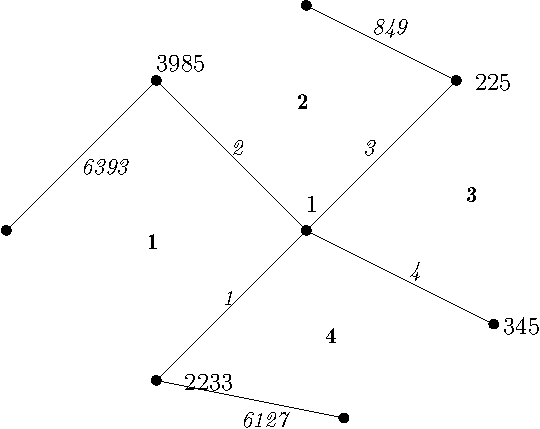
\includegraphics{Figures/dcel.pdf}
  \caption{The particle graph associated with the DCEL of Table~\ref{table:dcel}.
           The dots represent particle centers.  Lines represent the contacts between
           particles.}
           \label{fig:dcel}
\end{figure}
%
\begin{itemize}
\item
Row 3 in an F-file corresponds to contact 3
(see row~3 in Table~\ref{table:dcel}).
\item
Contact 3 is between particle number 1 (\texttt{V1})
and particle number 225 (\texttt{V2})
(i.e., rows 1 and 225 in the corresponding Fb-file).
\item
Void cell 2 (\texttt{F1}) lies on one side of this
contact, and void cell 3 lies on its other side (\texttt{F2}).
See Section~\ref{sec:ktype2} for a further description of void cells.
\item
Pointer \texttt{P1} (= 4) points to a contact (row 4),
which is also connected to \texttt{V1} (particle number 1)
and lies directly clockwise around \texttt{V1} relative to the 
row 3 contact.
\item
Pointer \texttt{P2} (= 849) points to the contact (row 849)
that is also connected to \texttt{V2} (= particle 225)
and lies clockwise around \texttt{V2} relative
to the third (row 3) contact.
\end{itemize}
The \texttt{hv} data in an Fb-files point to the starting
(header) contact for a
particle (Section~\ref{sec:f2files}).
With this data structure, you will be able to identify all of
the contacts that are connected to an arbitrary particle.
You will also be able to identify all contacts
and particles that lie around the perimeter of
a polygonal void cell.
That is, you can construct both the particle graph and its dual
\cite{Satake:1992a}.
The \texttt{hf} data in an Fd-file points to the starting
(header) contact for a
void cell (Section~\ref{sec:f4files}).
\par
The final seven columns in an Fc-file give the following data:
\begin{itemize}
\item
\texttt{branch(1)} and \texttt{branch(2)}:
the horizontal and vertical component of the branch vector that
connects 
the centers of particles \texttt{V1} and \texttt{V2}
(directed toward \texttt{V2}).  Note that the format of these two
fields is \texttt{1pe17.9}.
\item
\texttt{c\_eta(1)} and \texttt{c\_eta(2)}:
the horizontal and vertical components of the unit normal vector, directed
outward from the surface of particle \texttt{V1}
at the contact location.
\item
\texttt{fnold1(1)}:
the magnitude of the 
contact force component that acts normal to the contact surface---a
positive value for compressive contact force.
\item
\texttt{ftold(1)} and \texttt{ftold(2)}:
the horizontal and vertical components of the contact force
tangential to the contact surface.
The force acts upon particle \texttt{V1}.
\item
\texttt{Tstar}:
For Hertz-Mindlin contacts only (\texttt{imodel=5}, 
Section~\ref{sec:imodel}). See~\cite{Thornton:1988a}.
\end{itemize}
%
\subsubsection{Fc-files for 2D assemblies of non-convex particles}\label{sec:f3files2}
With non-convex particles, such as nobbies,
two particles can have multiple contacts between each other.
The Fc-file gives information identifies the two particles and their
component parts (satellite and central circles) that are touching.
Each line in the Fc-file has format
\texttt{4(i7)},\texttt{2(i8)},\texttt{2(1pe17.9)},
\texttt{i3},\texttt{4(i7,i3,i3)}
and contains the following information:
\begin{itemize}
\item
The first six fields contain \texttt{V1}, \texttt{V2}, \texttt{F1}, \texttt{F2}, \texttt{P1},
and~\texttt{P2}.
These are described in Section~\ref{sec:f3files}.
\item
The next two fields contact \texttt{branch(1)} and \texttt{branch(2)}
as described in Section~\ref{sec:f3files}.
\item
\texttt{ihit}: the number of contacts between these two particles.
\item
Four triples of integers.  With non-convex particles, such as nobbies,
two particles can have multiple contacts between each other.
Each triple corresponds to one of these contacts.
Each triple is composed of a pointer to
a position within the list of an ``Ff'' file and two identifiers
of the component circles that that are touching (one identifier for
the first particle \texttt{V1}, the other identifier for the
second particle \texttt{V2}).
The identifier is an integer ranging between 0 and \texttt{nobs}:
the zero corresponding to the central circle, numbers 1 and above
corresponding to the satellite circles (arcs).
If a pair of particles has fewer than four contacts, then
zeros will appear in the unused triples.
\end{itemize}
%
\subsubsection{Fd-files for 2D assemblies}\label{sec:f4files}
The lines of this file contain a single integer
in \texttt{i7} format.  The \texttt{hv} integer on 
each line is a pointer to the DCEL for a single void cell
(Section~\ref{sec:f3files}).
The lines are given in order (for example,
line 14 gives the \texttt{hv} value for void cell number 14).
%
\subsubsection{Ff-files for 2D assemblies}\label{sec:f6files2d}
These files are only created for non-convex particles, such
as nobbies.
Each line in this file gives information on a single contact.
Note that a pair of particles can share multiple contacts.
As described in Section~\ref{sec:f3files2},
Each pair of contacting particles will be represented with a 
single line in an Fc-file.
For non-convex particles, the Fc-file will identify the two particles
(the locations of these particles are given in the Fb-file), 
the branch vector between the particles' centers, 
number of contacts between the two particles,
and triple-integers that identify each of these contacts.
The first integer in a triple points to a line in the Ff-file.
The contents of the Ff-file depends on the contacts'
displacement-force model (\texttt{imodel}, Section~\ref{sec:imodel}).
%
\par
For nobby particles with a linear-frictional contact
model (\texttt{imodel=0}), 
this line has format \texttt{4(1pe17.9)}
and contains the following information about the contact:
\begin{itemize}
\item
The two components of the contact's normal vector (directed outward
from the first particle, \texttt{V1}).
\item
The normal force (compression is positive).
\item
The three components of the contact's tangential force
(acting upon the first particle, \texttt{V1}).
\end{itemize}
%
\par
For nobby particles with a simple Hertz-Mindlin
model (\texttt{imodel=5}), 
this line has format \texttt{5(1pe17.9)}
and contains the following information about the contact:
\begin{itemize}
\item
The two components of the contact's normal vector (directed outward
from the first particle, \texttt{V1}).
\item
The normal force (compression is positive).
\item
The three components of the contact's tangential force
(acting upon the first particle, \texttt{V1}).
\item
\texttt{Tstar}.
\end{itemize}
%
\par
For nobby particles with the J\"{a}ger\ contact
model (\texttt{imodel=6}), 
this line has format \texttt{7(1pe17.9)}
and contains the following information about the contact:
\begin{itemize}
\item
The two components of the contact's normal vector (directed outward
from the first particle, \texttt{V1}).
\item
The normal force (compression is positive).
\item
The three components of the contact's tangential force
(acting upon the first particle, \texttt{V1}).
\end{itemize}
%
\subsection{F-files for 3D assemblies}\label{sec:ffiles3d}
Four F-files are created at together (Table~\ref{table:ffiles}),
and they are described in the following three subsections:
Fa-files (Section~\ref{sec:f1files3d}),
Fb-files (Section~\ref{sec:f2files3d}),
Fc-files (Section~\ref{sec:f3files3d}),
and Ff-files (Section~\ref{sec:f6files3d}).

\subsubsection{Fa-files for 3D assemblies}\label{sec:f1files3d}
Same data as with 2D assemblies (Section~\ref{sec:f1files}).
%
\subsubsection{Fb-files for 3D assemblies}\label{sec:f2files3d}
These files contain information on the size and position of each particle.
Each line gives data for a single particle, with the
lines arranged by particle number (line number 3 in the file is 
for particle~3).
\par
For 3D assemblies of spheres,
the format of each line is \texttt{4(1pe17.9),3(1pe18.9e3)}, with
the following fields 
for each sphere:\\
\begin{center}
\begin{tabular}{lp{3.5in}}
Field 1 & radius \\
Field 2 & $x_{1}$ position of the particle center\\
Field 3 & $x_{2}$ position of the particle center\\
Field 4 & $x_{3}$ position of the particle center\\
Field 5 & $\theta_{1}$ angular orientation of the particle (radians)\\
Field 6 & $\theta_{2}$ angular orientation of the particle (radians)\\
Field 7 & $\theta_{3}$ angular orientation of the particle (radians)
\end{tabular}
\end{center}
\par
For 3D assemblies of ovoids,
the format of each line is \texttt{7(1pe17.9),3(1pe18.9e3)}, with
the following fields
for each ovoid:\\
\begin{center}
\begin{tabular}{lp{3.5in}}
Field 1 & transverse (revolved) half width (Section~\ref{sec:ovoid_data})\\
Field 2 & aspect ratio:  axial height / transverse width \\
Field 3 & $x_{1}$ position of the particle center\\
Field 4 & $x_{2}$ position of the particle center\\
Field 5 & $x_{3}$ position of the particle center\\
Field 6 & $\gamma_{1}$ orientation angle (in degrees) of
the particle's axis,
(Fig.~\ref{fig:coordinates}, Section~\ref{sec:ovoid_data})\\
Field 7 & $\gamma_{2}$ orientation angle (in degrees) of
the particle's axis,
(Fig.~\ref{fig:coordinates}, Section~\ref{sec:ovoid_data})\\
Field 8 & $\theta_{1}$ angular orientation of the particle (radians)\\
Field 9 & $\theta_{2}$ angular orientation of the particle (radians)\\
Field 10 & $\theta_{3}$ angular orientation of the particle (radians)
\end{tabular}
\end{center}
\par
For 3D assemblies of bumpies,
the format of each line is \texttt{4(1pe17.9),4(1pe18.9e3)}, with
the following fields
for each ovoid:\\
\begin{center}
\begin{tabular}{lp{3.5in}}
Field 1 & scaling radius (Sections~\ref{sec:satrad} 
          and~\ref{sec:bumpy_data})\\
Field 2 & $x_{1}$ position of the particle center\\
Field 3 & $x_{2}$ position of the particle center\\
Field 4 & $x_{3}$ position of the particle center\\
Field 5 & 1st component of the unit orientation quaternion\\
Field 6 & 2nd component of the unit orientation quaternion\\
Field 7 & 3rd component of the unit orientation quaternion\\
Field 8 & 4th component of the unit orientation quaternion
\end{tabular}
\end{center}
%
\subsubsection{Fc-files for 3D assemblies}\label{sec:f3files3d}
Each line in this file gives information on a single contact.
\par
For 3D assemblies of spheres,
the format of each line is \texttt{2i7,},\texttt{3(1pe17.9)},
\texttt{4(1pe13.5)}, with
the following fields for each sphere
(with Hertz-Mindlin contacts, the value of \texttt{Tstar} in
format \texttt{1pe13.5} is included at the end of a line):
\begin{itemize}
\item
\texttt{V1} and \texttt{V2}:
the two particle numbers
\item
\texttt{branch(1)}, \texttt{branch(2)}, and \texttt{branch(3)}:
the components of the branch vector that
connects the centers of particle \texttt{V1} and particle \texttt{V2}
(directed toward \texttt{V2}).  Note that the format for these three fields
is \texttt{1pe16.8}.
\item
\texttt{fnold1(1)}:
the magnitude of the contact force 
component that acts normal to the contact surface---a
positive value for compressive forces.
\item
\texttt{ftold(1)}, \texttt{ftold(2)}, and \texttt{ftold(3)}:
the three components of the portion of the contact force
that is tangential to the contact surface.
The force acts upon particle \texttt{V1}.
\item
\texttt{Tstar}:
For Hertz-Mindlin contacts only (\texttt{imodel=5},
Section~\ref{sec:imodel}). See~\cite{Thornton:1988a}.
\end{itemize}
%
\par
For 3D assemblies of ovoids,
the format of each line is \texttt{2i7},\texttt{3(1pe17.9)},
\texttt{10(1pe13.5)},with
the following fields
for each ovoid
(with Hertz-Mindlin contacts, the value of \texttt{Tstar} in
format \texttt{1pe13.5} is included at the end of a line):
\begin{itemize}
\item
\texttt{V1} and \texttt{V2}:
the two particle numbers.
\item
\texttt{branch(1)}, \texttt{branch(2)}, and \texttt{branch(3)}:
the components of the branch vector that
connects the centers of particle \texttt{V1} and particle \texttt{V2}
(directed toward \texttt{V2}).  Note that the format for these three fields
is \texttt{1pe17.9}.
\item
\texttt{rx\_i(1)}, \texttt{rx\_i(2)}, and \texttt{rx\_i(3)}:
The components of a vector from the center of particle \texttt{V1}
to the center of the contact point between the two particles.
\item
\texttt{fnold1(1)}:
the magnitude of the contact force
component that acts normal to the contact surface---a
positive value for compressive contact force.
\item
\texttt{ftold(1)}, \texttt{ftold(2)}, and \texttt{ftold(3)}:
the three components of the portion of the contact force
that is tangential to the contact surface.
The tangential force acts upon particle \texttt{V1}.
\item
\texttt{c\_eta(1)}, \texttt{c\_eta(2)}, and \texttt{c\_eta(3)}:
The three components of the unit vector that is the outward normal
of particle \texttt{V1} at the contact point.
\item
\texttt{Tstar}:
For Hertz-Mindlin contacts only (\texttt{imodel=5},
Section~\ref{sec:imodel}). See~\cite{Thornton:1988a}.
\end{itemize}
%
\par
For 3D assemblies of bumpies,
the format of each line is \texttt{2i7},\texttt{3(1pe17.9)},
\texttt{i3},\texttt{6(i7,i3,i3)}, with
the following fields for each bumpy:
\begin{itemize}
\item
\texttt{V1} and \texttt{V2}:
the two particle numbers.
\item
\texttt{branch(1)}, \texttt{branch(2)}, and \texttt{branch(3)}:
the components of the branch vector that
connects the centers of particle \texttt{V1} and particle \texttt{V2}
(directed toward \texttt{V2}).  Note that the format for these three fields
is \texttt{1pe17.9}.
\item
\texttt{ihit}: the number of contacts between these two particles.
\item
Six triples of integers.  With non-convex particles, such as bumpies,
two particles can have multiple contacts between each other.
Each triple corresponds to one of these contacts.
Each triple is composed of a pointer to
a position within the list of an ``Ff'' file and two identifiers 
of the component spheres that that are touching (one identifier for
the first particle \texttt{V1}, the other identifier for the
second particle \texttt{V2}).
The identifier is an integer ranging between 0 and \texttt{nbumps}:
the zero corresponding to the central sphere, numbers 1 and above 
corresponding to the satellite spheres.
\end{itemize}
%
\subsubsection{Ff-files for 3D assemblies}\label{sec:f6files3d}
These files are only created for non-convex particles, such
as bumpies.
Each line in this file gives information on a single contact.
Note that a pair of particles can share multiple contacts.
As described in Section~\ref{sec:f3files3d},
Each pair of contacting particles will be represented with a 
single line in an Fc-file.
For non-convex particles, the Fc-file will identify the two particles
(the locations of these particles are given in the Fb-file), 
the branch vector between the particles' centers, 
number of contacts between the two particles,
and triple-integers that identify each of these contacts.
The first integer in a triple points to a line in the Ff-file.
The contents of the Ff-file depends on the contacts'
displacement-force model (\texttt{imodel}, Section~\ref{sec:imodel}).
%
\par
For bumpy particles with a linear-frictional contact
model (\texttt{imodel=0}), 
this line has format \texttt{4(1pe17.9)}
and contains the following information about the contact:
\begin{itemize}
\item
The normal force (compression is positive).
\item
The three components of the contact's tangential force
(acting upon the first particle, \texttt{V1}).
\end{itemize}
%
\par
For bumpy particles with a simple Hertz-Mindlin
model (\texttt{imodel=5}), 
this line has format \texttt{5(1pe17.9)}
and contains the following information about the contact:
\begin{itemize}
\item
The normal force (compression is positive).
\item
The three components of the contact's tangential force
(acting upon the first particle, \texttt{V1}).
\item
\texttt{Tstar}.
\end{itemize}
%
\par
For bumpy particles with the J\"{a}ger\ contact
model (\texttt{imodel=6}), 
this line has format \texttt{7(1pe17.9)}
and contains the following information about the contact:
\begin{itemize}
\item
The three components of the contact's normal vector (directed outward
from the first particle, \texttt{V1}).
\item
The normal force (compression is positive).
\item
The three components of the contact's tangential force
(acting upon the first particle, \texttt{V1}).
\end{itemize}
%
%
\section{Screen output from \Oval}\label{sec:ScreenOval}
As a simulation is running, information is printed to the screen, which
can help to monitor the performance of the run.
This information can, of course, 
alternatively be redirected from the screen 
to a file.
The following is an example of the introductory information that might
appear on the screen at the beginning of a simulation:
\par
\footnotesize
\begin{verbatim}
Program OVAL:  version            oval-0.5.41.f
c Matthew R. Kuhn 2001, Licensed under the GPL, version 2

The program was compiled under the following parameters:
   1) 2D or 3D problems. (mdim1=3)
   2) Circular, spherical, elliptical, oval, and ovoid particles. (mpiece=4*mp)
   3) A maximum of 10020 particles. (mp)
Errors will occur if your input data is otherwise (but you can always make
changes to the common-0.5.41 file and recompile).
  
  Name of the RunFile:
LoadComp                 <-- your input here
  Name of the StartFile:
Dsphere_1800             <-- your input here
  
 **** Warning ****.
 * The input value of rho was 0.
 * A mass will be automatically assigned.
  
 **** Warning ****.
 * The input value of dt was 0.
 * A time step will be automatically assigned.

  Your time step is:                1.00000E+00
  The maximum advised time step is: 1.25000E+00

  The assigned particle mass is:    9.76563E+00

  Spherical, 3D particles

  Number of particles     =    1800
  Initial void ratio      =  0.535828
  Initial solids fraction =  0.651115
  Initial porosity        =  0.348885
  Volume of the cell      =  2.248245E+03

  Initial number of contacts       =    5130
  Average ratio of overlap/diameter =  3.186E-04
\end{verbatim}
\normalsize
\par
In this example, the names of the two input files are \texttt{Load1}
and \texttt{Dcircls\_1002}.
The introductory information is followed by a table of diagnostic
information that is periodically updated at the interval \texttt{ipts}, as
specified in the \textsf{RunFile} (Section~\ref{sec:ipts}).
This table will look something like the following:
\par
\footnotesize
\label{verb:screen2}
\begin{verbatim}
Some diagnostic information during this run:
iout    timer istep nupd  ipt2 xloops   chi1      chi2       psi    sweep
   0  0.0000E+00  1    1  18108   1.0  0.00E+00  0.00E+00  0.00E+00  0.00
   1  2.0000E+00  1    1  18108  21.5  1.10E-02  7.73E-03  0.00E+00  0.00
   2  4.0000E+00  1    1  18108   3.0  9.81E-03  7.04E-03  0.00E+00  0.00
   3  6.0000E+00  1    1  18108   3.0  8.79E-03  6.34E-03  0.00E+00  0.00
   4  8.0000E+00  1    1  18108   3.0  7.98E-03  5.74E-03  0.00E+00  0.00
   5  1.0000E+01  2    1  18108   3.0  7.14E-03  5.15E-03  0.00E+00  0.00
   6  5.8000E+01  2    2  18109   2.9  2.42E-03  1.77E-03  3.68E-06  0.00
   7  1.0800E+02  2    2  18109   3.0  3.55E-04  3.77E-04  1.39E-06  0.00
   8  1.5800E+02  2    3  18109   3.0  2.68E-04  3.38E-04  1.17E-06  0.00
\end{verbatim}
\normalsize
Most items in the table were described in
Section~\ref{sec:bfile2d}.
The integer \texttt{istep} is the current
deformation-stress segment
(from the \textsf{RunFile}, Section~\ref{sec:runfile2}).
The integer \texttt{nupdat} is the number of near-neighbor searches that
have been performed (see Section~\ref{sec:search}).
The integer \texttt{ipt2} is the current length of the near-neighbor
linked list (Section~\ref{sec:search}).
The value \texttt{xloops} is the average number of iteration loops
(time steps) per deformation step.  When \texttt{algori=1}, then
\texttt{xloops} will always be one.
The values \texttt{}, \texttt{}, and \texttt{} indicate the 
numeric performance of the run (see Sections~\ref{sec:chi1}, \ref{sec:chi2}, 
and \ref{sec:psi} and the other sections referenced from there).
The value \texttt{sweep} is the average number of iterations per
torus-torus contact when ovoids are being used.
%
%
\section{Sample assemblies for \Oval}\label{sec:samples}
You can download sample \textsf{StartFile} assemblies, 
which are given in a D-file (text) format,
from the web site given on page~\pageref{page:WebSite}.
The sample \StartFile s should be located in your \texttt{oval}
directory in 
\begin{verbatim}
    samples/startfiles
\end{verbatim}
The primary attributes of these assemblies 
are shown in Table~\ref{table:assemblies}.
\begin{table}
\centering
\begin{tabular}{lccccc}
\hline
\hline
          & Particle & No. of & Void  & Coord. & Dimensionless \\
File Name &   Type   & Particles & Ratio &   Number$^{5}$    &  Overlap      \\
\hline
\texttt{Dcircls\_1002\_2}$^{1}$&circles&1002&0.18042 &3.820 & 3.10$\times10^{-4}$\\
\texttt{Dcircls\_4008\_2}$^{1}$&circles&4008&0.17911 &3.813 & 3.19$\times10^{-4}$\\
\texttt{Dovals\_1002\_1d}      &ovals  &1002&0.18382 &3.784 & 2.32$\times10^{-4}$\\
\texttt{Dovals\_1002\_2d}      &ovals  &1002&0.12890 &4.880 & 1.58$\times10^{-4}$\\
\texttt{Dovals\_4008\_1d}      &ovals  &4008&0.18479 &3.777 & 2.10$\times10^{-4}$\\
\texttt{Dovals\_4008\_2d}      &ovals  &4008&0.12788 &4.733 & 1.72$\times10^{-4}$\\
\texttt{Dsphere\_1800}         &spheres&1800&0.53583 &5.700 & 3.19$\times10^{-4}$\\
\texttt{DOblate\_1800}$^{2}$   &ovoids &1800&0.41520 &8.214 & 1.65$\times10^{-4}$\\
\texttt{DProlate\_1800}$^{3}$  &ovoids &1800&0.41223 &8.438 & 2.01$\times10^{-4}$\\
\texttt{DObProlate\_1800}$^{4}$&ovoids &1800&0.41367 &8.351 & 2.01$\times10^{-4}$\\
\hline
\multicolumn{6}{l}{\parbox{4.80in}{%
$^{1}$The assemblies \texttt{Dcircls\_1002} and 
 \texttt{Dcircls\_4008} in \Oval\ version \texttt{0.4.0} have been
replaced.  These older assemblies were slightly anisotropic.}}\\
\multicolumn{6}{l}{\parbox{4.80in}{%
$^{2} $Oblate ovoids with randomly assigned aspect ratios.  
The aspect ratio is uniformly distributed between 0.65 and 1.00.%
}}\\
\multicolumn{6}{l}{\parbox{4.80in}{%
$^{3} $Prolate ovoids with randomly assigned aspect ratios.
The aspect ratio is uniformly distributed between 1.00 and 1.60.%
}}\\
\multicolumn{6}{l}{\parbox{4.80in}{%
$^{4} $A combination of oblate and prolate ovoids with 
randomly assigned aspect ratios.
The aspect ratio is uniformly distributed between 0.65 and 1.60.%
}}\\
\multicolumn{6}{l}{\parbox{4.80in}{%
$^{5} $The coordination number is computed as twice the number of contacts
divided by the number of particles.
}}\\
\hline
\hline
\end{tabular}
\caption{Attributes of several sample assemblies}
\label{table:assemblies}
\end{table}
Each assembly is roughly square (or cubical)
and with an isotropic fabric.
They were created by isotropically compressing a sparse assembly with
friction turned off.
\par
The assemblies contain a range of particles sizes.
The dimensions of the particles and the entire assemblies have
been scaled so that the mean particle size 
$D_{50}$ in each assembly is 1.00.
(\label{page:d50}Here, 
we speak of the mean particle size $D_{50}$ in the usual sense
of geotechnical engineering:  a ``median'' diameter that partitions
the assembly into two sets of particles, so that each set has an equal
cumulative mass.)
A density plot (normalized histogram) of 
particle radii for both 2D and 3D assemblies is shown
in Fig.~\ref{fig:radii}.  
\begin{figure}
\centering
\subfigure[2D assemblies]
{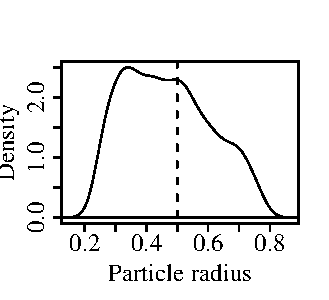
\includegraphics{Figures/radius}}%
\subfigure[3D assemblies]
{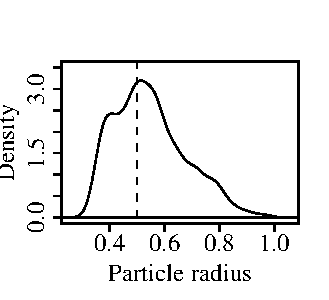
\includegraphics{Figures/radius3d}}%
\caption{Histograms of particle radii for 2D and 3D assemblies}
\label{fig:radii}
\end{figure}
The histogram is centered on the median size $0.50D_{50}$.
In Fig.~\ref{fig:radii}a, the radii of non-circular 2D particles 
refers to their mean radii, $(\mathrm{Height} + \mathrm{Width})/4$
(Fig.~\ref{fig:orientation_angle}, Section~\ref{sec:StartFile2}).
In Fig.~\ref{fig:radii}b, the radii of non-spherical 3D particles
refers to their mean radii, $(\mathrm{Height} + 2\cdot\mathrm{Width})/6$
The distribution of aspect ratios for oval and ovoid assemblies
are described in the footnotes of Table~\ref{table:assemblies}.
\par
The void ratio is a measure of the packing density of 
a granular assembly (Table~\ref{table:assemblies}).
The assemblies of circles, spheres, and ovoids are fairly dense.
Both loose and dense assemblies of ovals are provided.
The coordination numbers shown in Table~\ref{table:assemblies}
are computed as
twice the number of contacts divided by the number of particles.
\par
Among the attributes listed in Table~\ref{table:assemblies},
the dimensionless overlap probably has the greatest effect on
the speed and performance of a simulation.
The dimensionless overlaps, which are quite small, were computed
by dividing the average overlap at the particle contacts by the
mean particle size, $D_{50}$.
Small overlaps more closely resemble those in real 
granular materials, which are often composed of hard granules.
During simulations, however, small overlaps
require slower deformation rates to assure the near quasi-static
progression of particle rearrangements.
\par
In addition to the files in Table~\ref{table:assemblies},
the website includes a directory 
\texttt{samples/startfiles/Series\_circls\_1002/}
that contains 100 assemblies of 1002 circular particles.
The particle size distribution in each assembly is the same as that of
\texttt{Dcircls\_1002\_2} in Table~\ref{table:assemblies}
and Fig.~\ref{fig:radii}a.
Each assembly has exactly the same particle sizes and the same void 
ratio (=0.174257), but the assemblies have different particle arrangements.
As a result of this difference, the files will have modest differences
in the number of contact, dimensionless overlap, and initial stress.
The assemblies were constructed with the same process, but the
the particle radii were shuffled among the particles before
the diffuse assembly was compacted.
%
%
\section{Example simulations using \Oval}
As an example simulation, consider the \textsf{RunFile}
named \texttt{LoadComp}
shown on page~\pageref{fig:LoadComp}.
After a brief initial period in which the assembly is allowed to
equilibrate,
the assembly is vertically compressed while maintaining constant
horizontal stress ($\dot{F}_{22}<0$, $\dot{F}_{11}=0$).
For 3D assemblies, the deformations were under 
plane strain conditions ($\dot{F}_{33}=0$).
The results for all of the larger assemblies are shown in
Fig.~\ref{fig:results_all}
\begin{figure}\small
\centering
\subfigure[]
{% GNUPLOT: LaTeX picture with Postscript
\begingroup%
  \makeatletter%
  \newcommand{\GNUPLOTspecial}{%
    \@sanitize\catcode`\%=14\relax\special}%
  \setlength{\unitlength}{0.1bp}%
\begin{picture}(2519,1620)(0,0)%
\special{psfile=Stress_all.ps llx=0 lly=0 urx=504 ury=378 rwi=5040}
\put(1569,413){\makebox(0,0)[l]{1800 spheres}}%
\put(1569,513){\makebox(0,0)[l]{4008 ovals, dense}}%
\put(1569,613){\makebox(0,0)[l]{4008 ovals, loose}}%
\put(1569,713){\makebox(0,0)[l]{4008 circles}}%
\put(1384,50){\makebox(0,0){Vertical strain, $\varepsilon_{22}$}}%
\put(100,910){%
\special{ps: gsave currentpoint currentpoint translate
270 rotate neg exch neg exch translate}%
\makebox(0,0)[b]{\shortstack{Deviator stress, $(\sigma_{22}-\sigma_{11})/p_{\mathrm{o}}$}}%
\special{ps: currentpoint grestore moveto}%
}%
\put(2272,200){\makebox(0,0){0.005}}%
\put(1877,200){\makebox(0,0){0.004}}%
\put(1483,200){\makebox(0,0){0.003}}%
\put(1089,200){\makebox(0,0){0.002}}%
\put(694,200){\makebox(0,0){0.001}}%
\put(300,200){\makebox(0,0){0}}%
\put(250,1520){\makebox(0,0)[r]{4}}%
\put(250,1215){\makebox(0,0)[r]{3}}%
\put(250,910){\makebox(0,0)[r]{2}}%
\put(250,605){\makebox(0,0)[r]{1}}%
\put(250,300){\makebox(0,0)[r]{0}}%
\end{picture}%
\endgroup
\endinput
}\\
\subfigure[]
{% GNUPLOT: LaTeX picture with Postscript
\begingroup%
  \makeatletter%
  \newcommand{\GNUPLOTspecial}{%
    \@sanitize\catcode`\%=14\relax\special}%
  \setlength{\unitlength}{0.1bp}%
\begin{picture}(2519,1511)(0,0)%
\special{psfile=Volume_all.ps llx=0 lly=0 urx=504 ury=353 rwi=5040}
\put(963,998){\makebox(0,0)[l]{1800 spheres}}%
\put(963,1098){\makebox(0,0)[l]{4008 ovals, dense}}%
\put(963,1198){\makebox(0,0)[l]{4008 ovals, loose}}%
\put(963,1298){\makebox(0,0)[l]{4008 circles}}%
\put(1509,50){\makebox(0,0){Vertical strain, $\varepsilon_{22}$}}%
\put(100,855){%
\special{ps: gsave currentpoint currentpoint translate
270 rotate neg exch neg exch translate}%
\makebox(0,0)[b]{\shortstack{Volume strain, $\frac{1}{2}\varepsilon_{kk}$ or $\frac{1}{3}\varepsilon_{kk}$}}%
\special{ps: currentpoint grestore moveto}%
}%
\put(2295,200){\makebox(0,0){0.005}}%
\put(1946,200){\makebox(0,0){0.004}}%
\put(1597,200){\makebox(0,0){0.003}}%
\put(1248,200){\makebox(0,0){0.002}}%
\put(899,200){\makebox(0,0){0.001}}%
\put(550,200){\makebox(0,0){0}}%
\put(500,1411){\makebox(0,0)[r]{0.006}}%
\put(500,1252){\makebox(0,0)[r]{0.005}}%
\put(500,1094){\makebox(0,0)[r]{0.004}}%
\put(500,935){\makebox(0,0)[r]{0.003}}%
\put(500,776){\makebox(0,0)[r]{0.002}}%
\put(500,617){\makebox(0,0)[r]{0.001}}%
\put(500,459){\makebox(0,0)[r]{0}}%
\put(500,300){\makebox(0,0)[r]{-0.001}}%
\end{picture}%
\endgroup
\endinput
}
\caption{Results for both 2D and 3D materials: deviator stress and volumetric
behavior.}
\label{fig:results_all}
\end{figure}
and are archived at the web site (page~\pageref{page:WebSite}).
These results can also be found in the your \texttt{oval} directory in
\begin{verbatim}
    samples/results
\end{verbatim}
The deviator stress in Fig.~\ref{fig:results_all} has been normalized by
dividing by the initial mean stress, $p_{\mathrm{o}}$.
Note the quite large difference in strengths of the
loose and dense assemblies of ovals.
The loose assembly (created quite by accident)
is much weaker than the assembly of circular discs, even though
the two assemblies have nearly the same void ratio.
The strength of the 3D assembly of spheres is much larger than
that of the 2D assembly of circles, which is due, in part, to the
plane strain conditions during compression of the 3D assembly.
The execution times for the three 
tests are shown in Table~\ref{fig:runtimes},
\begin{table}
\centering
\begin{tabular}{lccl}
\hline
\hline
Start File& Particle & No. of    & Run  \\
Name      &   Type   & Particles & Time \\
\hline
\texttt{Dcircls\_4008}   & circles & 4008 & 19m\ 52s\\
\texttt{Dovals\_1002\_2} & ovals   & 1002 &  9m\ 51s \\
\texttt{Dovals\_4008\_2} & ovals   & 4008 & 43m\ 10s \\
\texttt{Dsphere\_1800}   & spheres & 1800 & 19m\ 21s \\
\hline
\hline
\end{tabular}
\caption{Execution times for simulations with
the \textsf{RunFile} shown in Fig.~\ref{fig:LoadComp},
page~\pageref{fig:LoadComp} and various 
\textsf{StartFile} assemblies (Table~\ref{table:assemblies}).
The times are with an Intel Pentium~III 450MHz processor.}
\label{fig:runtimes}
\end{table}
using an Intel Pentium~III 450MHz machine and executable binaries
produced by the pgf77 Linux compiler.
As can be seen in the table, the execution time is roughly proportional to the
number of particles.
Oval particles require about twice the time of circular particles.
Spherical particles also require about twice the time of circular particles.
%
%
\section{Some advice on using \Oval}\label{sec:advice}
When \Oval\ is properly used, the program is efficient and provides
repeatable results.
The program can be maddening, however, when it is unknowingly being stretched
beyond its limits.
You may want to consider the following advice.
\begin{enumerate}
\item\label{item:slowisbetter}
Slow is (usually) better.
When choosing deformation or stress rates with the
input values \texttt{defrat(i,j)}, the program's performance
can be greatly improved by choosing appropriately slow rates
(Section~\ref{sec:icontr} and~\ref{sec:defrat}).
What is an appropriate rate?
If the rate is too slow, you will needlessly waste time (days, weeks,
months) waiting for your simulation to finish.
If the rate is too fast, the program will either fail to maintain
quasi-static conditions (when \texttt{algori=1}, 
Section~\ref{sec:algori}), will run
excessively slow while attempting to establish quasi-static conditions
(when \texttt{algori=2}), or will crash.
A common error message upon crashing is the following:
\begin{verbatim}
    An illegitimate contact in subroutin lister.
\end{verbatim}
This error occurs when the particle velocities are excessive, causing 
two particles that were previously not even in the linked-list
of near-neighbors to come into contact within a single time step
(Section~\ref{sec:search}).
\Oval\ will not stop running, but if this message repeatedly occurs or
the results become erratic, you will probably want to reduce the deformation
rate.
(I am fairly tolerant of this error when I am not particularly interested
in the accuracy of the results, for example when I am preparing an assembly
from a sparse arrangement of particles.)
\par
The proper deformation rate depends primarily on (and is 
almost proportional to)
the average overlap among particles in their initial configuration.
If the overlaps are too large (relative to the particle radii), 
the simulation will not be very realistic.
With smaller average overlaps, slower deformation rates will be required
to maintain nearly quasi-static conditions.
Note that the relative overlaps are fairly small
for the sample assemblies that are included in the \Oval\ package
(Table~\ref{table:assemblies}, page~\pageref{table:assemblies}).
\par
The best way to determine a suitable deformation rate may be by trial
and error.
If you are testing an initially dense assembly,
choose \texttt{algori=2} and try a few \texttt{defrat} values.
The first deformation-stress control segment, however, should 
not involve any deformation.  
A beginning period of quiescence is required to allow the initial particle 
arrangement to come to near-equilibrium.
The first segment should, therefore, have
\texttt{icontr=000000} and should be long enough
(\texttt{igoal=70}, with sufficient time \texttt{finalv})
to allow a enough steps for the initial particle arrangement
to equilibrate (Sections~\ref{sec:igoal} and~\ref{sec:icontr}).
\par
The second and subsequent stress-deformation control segments are where you
can test the deformation rate.
As the program runs and output appears on the screen, 
wait until these segments are entered (see the \texttt{istep}
values on the screen output, page~\pageref{verb:screen2}),
and then monitor the values of
\texttt{chi1}, \texttt{chi2}, and \texttt{xloops}
(Sections~\ref{sec:chi1}, \ref{sec:chi2}, and~\ref{sec:xloops}).
The option \texttt{algori=2} provides a minimum 
of 3 equilibrating time steps per deformation step, with a maximum
of 101 time steps (Section~\ref{sec:algori}).
If \texttt{xloops} is consistently 3.0, you can probably increase
the trial deformation rate.
If \texttt{xloops} is consistently much greater than 3.0,
then the deformation rates are probably too high.
I usually try to keep \texttt{xloops} near 3 or 4 and
\texttt{chi1} and \texttt{chi2} below 0.005.
%
\item
For diffuse, sparse assemblies, use \texttt{algori=1} 
(Section~\ref{sec:algori}).
This will be the case if you are trying to compact a gaseous assembly
into a dense one.
For dense assemblies, use \texttt{algori=2},
as this will enforce a self-regulating mechanism for maintain
nearly quasi-static conditions.
%
%\item
%Use the standard DEM integration scheme (\texttt{iinteg=1},
%Section~\ref{sec:iinteg}) unless
%you wish to experiment in situations that are likely to develop
%large localization phenomena such as shear bands.
%
\item
I sometimes give the particles initial velocities (\texttt{rmsvel>0})
to help in densifying an initially loose particle arrangement.
As has already been stated, slow is usually better.
If you get the message,
\begin{verbatim}
    An illegitimate contact in subroutin lister.
\end{verbatim}
then you have probably assigned an \texttt{rmsvel} value that is
too large.
\item
When starting a simulation with a D-file or E-file, the
particles will likely not be in an equilibrium configuration,
since these files only specify the particle positions and provide
no information about the contact forces
(see \texttt{istart=3}, Section~\ref{sec:istart}).  
This means that the
initial calculation of contact forces will give zero tangential force,
a condition not likely to produce equilibrium.
The first deformation-stress segment, therefore, should
not involve any deformation.
Instead,
a beginning period of quiescence is required to allow for the initial particle
arrangement to come to near-equilibrium.
The first segment should, therefore, have
\texttt{icontr=000000} and should be long enough
(\texttt{igoal=70}, with sufficient time \texttt{finalv})
to allow a few time steps for the initial particle arrangement
to equilibrate (Sections~\ref{sec:igoal} and~\ref{sec:icontr}).
The second and subsequent stress-deformation control segments are where you
can start the desired deformation process.
\item
Binary E-file and C-file formats might not be portable 
between different platforms or operating systems.
\item
If you are assigning initial random velocities to the particles
(an input value \mbox{\texttt{rmsvel}$\neq$\texttt{0}}), do not
assign velocities that are too large.
You will probably need to reduce the value of \texttt{rmsvel}
if you get the error message:
\begin{verbatim}
    An illegitimate contact in subroutine lister.
\end{verbatim}
See item~\ref{item:slowisbetter} above.
\item
\Oval\ does not work when the assembly contains too few particles,
say fewer than nine 2D particles or twenty-seven 3D particles.
This problem is related to the use of periodic boundaries.
As an example, consider a square arrangement of four particles of equal 
size with this arrangement:
%
\begin{center}
  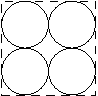
\includegraphics{Figures/four_circles}
\end{center}
%
Each particle touches a neighboring particle twice:
once within the core assembly and once again across a periodic
boundary.
\Oval's underlying data structure allows for a single contact per
particle pair.
This problem is avoided with a larger number of particles.
(Thanks to Csilla and Tam\'{a}s.)
\item
Do not try to control a boundary stress when the boundary stress
is zero.
For example, an input value \texttt{icontr=11100}
will not work with a diffuse, gaseous assembly
(Section~\ref{sec:icontr}).
\item\label{item:error2}
If you get an error message that your input files can not be properly read,
you will want to carefully check the formatting of the file's input
fields.
Microsoft Windows users may have problems with hidden characters that can
be embedded in files when using Word and Word Pad.
You will probably want to install a genuine text processor and
avoid using word processors.
%
\item\label{item:error10}
If at the start of a simulation you get the unexpected message,
``\texttt{Name of a platen file:}'', then you have probably given
\texttt{nplatn} a non-zero value in your 
\RunFile\ (see Section~\ref{sec:nplatn}).
%
\end{enumerate}
%
%
%
\section{Change Log}\label{sec:change_log}
This section documents the changes that have been made between various
version of \Oval\ and \OvalPlot.
\subsection{\Oval--0.4.0 to \Oval--0.6.0}\label{sec:oval04_to_oval06}
Added features:
\begin{itemize}
\item
Added the 3D non-spherical ovoid particle (Sections~\ref{sec:kshape},
\ref{sec:ovoid_data}, \ref{sec:f2files3d}).
\item
Added the ``krotat'' option of either allowing or preventing particle rotations
and/or particle translations (Section~\ref{sec:krotat}).
\item
Converted to list-directed input for D-files.  This allows
for much less restrictive input files (for example, input
files created with spreadsheets).
\item
Added more information printed to the screen at the start
of a run.
\item
Added the option of automatically computing the mass and/or the time step to
optimize performance (Sections~\ref{sec:dt}).
\item
Added the option of \texttt{nloop1} into the 
input \RunFile\ (Section~\ref{sec:nloop1}).
\end{itemize}
Enhancements:
\begin{itemize}
\item
Improved the near-neighbor search algorithm for ellipse, oval, and
ovoid particles.  
These changes should reduce the search time by up to a factor of 10.
\item
Added several hundreds of comments to the source code.
\end{itemize}
Bug fixes:
\begin{itemize}
\item
With 3D assemblies, print header line in B-files.
\item
Corrected output value of xloops in 3D B-files.
\item
Moved the code for repositioning ovals within the subroutines
``integ1'' and ``integ2''.  This change will be necessary for handling
non-periodic boundaries
\item
Previously, the particles were placed back into the main
periodic cell in subroutin ``lister'' whenever they drifted
outside the main cell.  What seemed like a nice act of
basic housekeeping actually produces problems with OvalPlot.
I eliminated this feature.
\item
Corrected an error in the handling of periodic boundaries in the
near-neighbor search subroutine ``lister''.
\end{itemize}
%
%
\subsection{\Oval--0.6.0 to \Oval--0.6.1}\label{sec:oval06_to_oval061}
Added features:
\begin{itemize}
\item
Added information contained in the A-file:
fabric tensor $\mathbf{A}$; fabric tensor of strong contacts $\mathbf{A}^{s}$;
proportion of strong contacts; numbers of edges, faces, and vertices
in the particle graph, etc.
(Section~\ref{sec:Afiles}).
\end{itemize}
%
Enhancements:
\begin{itemize}
\item
Changed the code for single-precision (4-byte) to double-precision
(8-byte) for all floating point numbers.
\item
Changed the labeling scheme for \texttt{C?}, \texttt{Fa?} files
(Sections~\ref{sec:idump}, \ref{sec:ffiles}, and Table~\ref{table:ffiles})
\item
Changed the names of F-files from \texttt{F1<}$\ldots$\texttt{>} 
to \texttt{Fa<}$\ldots$\texttt{>}, etc.
(Sections~\ref{sec:ffiles2d} and~\ref{sec:ffiles3d})
\end{itemize}
Bug fixes:
\begin{itemize}
\item
Fixed bug that prevented the creation of F-files for non-spherical particles.
\end{itemize}
%
%
\subsection{\Oval--0.6.1 to \Oval--0.6.2}\label{sec:oval061_to_oval062}
Added features:
\begin{itemize}
\item
F-files now give output of the ortientation angles of the particles.
\end{itemize}
%
Enhancements:
\begin{itemize}
\item
Increase the precision of output of some fields in F-files.
\item
Increased the precision of contact inquiry for ovoids.
\end{itemize}
%
Bug fixes:
\begin{itemize}
\item
Fixed calculation of the average overlap among particles.
\end{itemize}
%
\subsection{\Oval--0.6.2 to \Oval--0.6.3}\label{sec:oval062_to_oval063}
Bug fixes:
\begin{itemize}
\item
Changes to contact inquiry algorithm for ovoids.
\end{itemize}
%
\subsection{\Oval--0.6.3 to \Oval--0.6.4}\label{sec:oval063_to_oval064}
Enhancements:
\begin{itemize}
\item
Add more information about the simulation parameters in the 
``\texttt{Fa}''-files (the \texttt{beta} angle, \texttt{fn},
\texttt{ft}, \texttt{frict}, and stress).
\item
Changed all angles in the ``\texttt{Fb}''-files to radians 
($\gamma_{1}$, $\gamma_{2}$, and $\theta$).
\item
Changes to screen output during an \Oval\ run to accommodate larger simulations.
\end{itemize}
Bug fixes:
\begin{itemize}
\item
Slight change in algorithm for contact damping.
\end{itemize}
%
\subsection{\Oval--0.6.4 to \Oval--0.6.5}\label{sec:oval064_to_oval065}
Enhancements:
\begin{itemize}
\item
Increased precision (digits) in the ``\texttt{Fa}''-files.
\item
Improved stability of the ovoid contact detection algorithm.
\end{itemize}
%
%
\subsection{\Oval--0.6.5 to \Oval--0.6.8}\label{sec:oval065_to_oval068}
Enhancements:
\begin{itemize}
\item
Report the effective void ratio in the A-files.
\item
Added most of the B-file information to the A-files.
\item
Added the possibility of U- and V-files.
\end{itemize}
Bug fixes:
\begin{itemize}
\item
Corrected error in defining \texttt{kshape} when reading a dump file.
\item
Limit the number of error message that can be printed to the \texttt{errfile}.
Large numbers of error could previously fill a file system.
\item
Corrected an error in overflows of \texttt{chi1} and \texttt{chi2}.
\end{itemize}
%
%
\subsection{\Oval--0.6.8 to \Oval--0.6.10}\label{sec:oval068_to_oval0610}
Enhancements:
\begin{itemize}
\item
Added \texttt{ivers} to extend {\RunFile}s.
\item
Added Hertz-Mindlin contact.
\item
Added flexible boundary and several forms of rigid boundaries.
\item
Added the option \texttt{iexact} for exactly integrating the kinetics
of ovoid particles
\item
Added external code for generating random numbers.
\item
Added information to A-files: the number of sliding contacts, etc.
\end{itemize}
%
%
%
\bibliography{Kuhn}
%
%
\end{document}
